\documentclass[10pt]{article}		% sets document class
\usepackage[usenames,dvipsnames]{pstricks}
\usepackage{mathpazo}
\usepackage{epsfig}
\usepackage{pst-grad} 				% enables gradients
\usepackage{pst-plot} 				% enables axes
\usepackage[space]{grffile} 		% enables spaces in paths
\usepackage{etoolbox} 				% enables spaces in paths
\makeatletter 						% enables spaces in paths
\patchcmd\Gread@eps{\@inputcheck#1 }{\@inputcheck"#1"\relax}{}{}
\makeatother
\usepackage[margin=1.0in]{geometry}	% sets paper size
\usepackage{amssymb}				% enables formulas
\usepackage{amsmath}				% enables formulas
\usepackage[utf8]{inputenc}			% enables diacritical input
\usepackage{graphicx}				% enables graphics
\graphicspath{ {images/} }			% sets graphics path
\usepackage{chngcntr}				% enables counter
\counterwithin{table}{subsection}	% enables table pre-labels
\counterwithin{figure}{subsection}	% enables figure pre-labels
\usepackage[labelsep=endash, labelfont=bf, font=bf]{caption}	% sets figure and caption separator
%\usepackage{indentfirst}			% enables indent on first paragraphs
\linespread{1.1}					% sets spacing to 1.5
\setlength{\parskip}{0.5em}			% sets paragraph spacing to 1m
%\usepackage{times}					% sets font to times new roman
\usepackage{wrapfig}				% enables text wrapping around figures
\usepackage{gensymb}				% enables symbols
\usepackage{endnotes}				% enables endnotes
\usepackage{afterpage}				% enables afterpage capability
\setcounter{secnumdepth}{3}			% sets counter recognitions to sssection for label capability
\numberwithin{equation}{section}
\makeatletter						% set figure labels to center
\g@addto@macro\@floatboxreset\centering
\makeatother
\usepackage{setspace}				% enables environments for spacing
\usepackage{graphicx}				% allows table usage
\usepackage{hyperref}				% enables hyperlinks
\hypersetup{colorlinks=false, linkcolor=cyan, urlcolor=cyan, linktoc=page} % sets hyperlink colors
\usepackage{accents}				% enables accents
\usepackage{textcomp} 				% enables copyright
\usepackage{tabto}					% enables tabbing
\setlength\parindent{0pt}			% sets no indents
\usepackage[framed]{mcode} 			% enables code boxes
\usepackage{titlesec}				% enables title formatting
\titleformat{\part}{\filcenter\huge\bfseries}{}{}{}
\usepackage{float}
\newcommand{\pder}[2]{\frac{\partial#1}{\partial#2}}			% partial command
\newcommand{\psder}[2]{\dfrac{\partial^2#1}{\partial#2^2}}		% partial command
\newcommand{\ptder}[2]{\dfrac{\partial^3#1}{\partial#2^3}}		% partial command
\newcommand{\pfder}[2]{\dfrac{\partial^4#1}{\partial#2^4}}		% partial command
\newcommand{\pdx}{\frac{\partial}{\partial x}}					% partial command
\newcommand{\pdy}{\frac{\partial}{\partial y}}					% partial command
\newcommand{\pdz}{\frac{\partial}{\partial z}}					% partial command

\begin{document}

\newcommand{\stoptocwriting}{%
	\addtocontents{toc}{\protect\setcounter{tocdepth}{-5}}}
\newcommand{\resumetocwriting}{%
	\addtocontents{toc}{\protect\setcounter{tocdepth}{\arabic{tocdepth}}}}

\stoptocwriting
\part*{\underline{AERO 430 -- Numerical Simulation} \\ \Large Finite Difference Method for the Two-Dimensional Orthotropic Laplace Equation Boundary-Value Problem \\ \large Ross B. Alexander}
\resumetocwriting

\vfill

\begin{figure}[h]
	\begin{center}
	\includegraphics[width = 0.8\linewidth]{analytical_surface_k_1}
	\end{center}
\end{figure}

\vspace{80pt}

\newpage

\tableofcontents

\newpage

\section{Orthotropic Diffusion Equation}

The orthotropic Laplacian boundary-value problem consists of:
\begin{itemize}
	\item the second-order linear partial differential equation:
	\begin{equation}
	\nabla \cdot (\mathbf{D} \nabla u) = 0 \qquad x,y \in [0, 1] \times [0, 1]
	\end{equation}
	\item the orthotropic diffusivity tensor:
	\begin{equation}
	\mathbf{D} = \begin{bmatrix}
	k^2 & 0 & 0 \\
	0 & 1 & 0 \\
	0 & 0 & 0
	\end{bmatrix}
	\end{equation}
	\item the simplified second-order linear partial differential equation:
	\begin{equation}
	k^2\psder{u}{x} + \psder{u}{y} = 0 \qquad x,y \in [0, 1] \times [0, 1]
	\end{equation}
	\item the boundary conditions:
	\begin{equation}
	\begin{split}
	u(x, 0) = 0 \qquad \qquad u(0, y) = 0  \\
	u(x, 1) = \sin{\pi x} \qquad u(1, y) = 0
	\end{split}
	\end{equation}
\end{itemize}

The physical model of the orthotropic diffusion equation is that of:
\begin{itemize}
	\begin{spacing}{0.5}
	\item electrical conduction through a medium that has orthotropic electrical conductivity
	\item magnetism of a material that has orthotropic magnetic permeability
	\item thermal conduction through a material that has orthotropic thermal conductivity
	\item diffusion through a fluid that has orthotropic diffusivity
	\end{spacing}
\end{itemize}

\newpage

\section{Analytical Solutions}

\subsection{Analytical Solution of the Orthotropic Diffusion Equation}

The orthotropic diffusion equation and boundary conditions for the 2-D model problem are:
\begin{equation}
k^2\psder{u}{x} + \psder{u}{y} = 0 \qquad x,y \in [0, 1] \times [0, 1]
\end{equation}
\begin{equation}
\begin{split}
u(x, 0) = 0 \qquad \qquad \quad u(0, y) = 0  \\
u(x, 1) = \sin(\pi x) \qquad \; u(1, y) = 0
\end{split}
\end{equation}
The following equation is the solution to the orthotropic diffusion equation with given boundary conditions:
\begin{equation}
\mathbf{u(x, y) = \frac{sin(\pi x) sinh(k\pi y)}{sinh(k\pi)}}
\end{equation}

The solution is plotted for $k=1$ and $k=10$.

\begin{figure}[H]
	\begin{center}
		\includegraphics[width = 0.39\linewidth]{analytical_surface_k_1}
		\includegraphics[width = 0.39\linewidth]{analytical_contour_k_1}
		\caption{Analytical Solution to the 2D Orthotropic Laplacian with $k = 1$}
	\end{center}
\end{figure}

\begin{figure}[H]
	\begin{center}
		\includegraphics[width = 0.39\linewidth]{analytical_surface_k_10}
		\includegraphics[width = 0.39\linewidth]{analytical_contour_k_10}
		\caption{Analytical Solution to the 2D Orthotropic Laplacian with $k = 10$}
	\end{center}
\end{figure}

\subsubsection{Proof of PDE Satisfaction}

The solution to the orthotropic diffusion equation is verified in the following discussion. The second partial derivatives are:
\begin{equation}
\begin{bmatrix}
\psder{u}{x} \\[12pt] \psder{u}{y}
\end{bmatrix} = \begin{bmatrix}
\dfrac{-\pi^2 \sin(\pi x) \sinh(k\pi y)}{\sinh(k\pi)} \\[12pt] \dfrac{k^2\pi^2\sin(\pi x) \sinh(k \pi y)}{\sinh(k\pi)}
\end{bmatrix}
\end{equation}
Then, replacing the partial derivatives in the orthotropic diffusion equation:
\begin{equation}
k^2\psder{u}{x} + \psder{u}{y} = 0
\end{equation}
\begin{equation}
k^2\left(\dfrac{-\pi^2 \sin(\pi x) \sinh(k\pi y)}{\sinh(k\pi)}\right) + \left(\dfrac{k^2\pi^2\sin(\pi x) \sinh(k \pi y)}{\sinh(k\pi)}\right) = 0 
\end{equation}
\begin{equation}
-\left(\dfrac{k^2\pi^2 \sin(\pi x) \sinh(k\pi y)}{\sinh(k\pi)}\right) + \left(\dfrac{k^2\pi^2\sin(\pi x) \sinh(k \pi y)}{\sinh(k\pi)}\right) = 0 
\end{equation}

Thus, the solution satisfies the partial differential equation.

\subsubsection{Proof of Boundary Condition Satisfaction}

The solutions to the boundary conditions of the orthotropic diffusion equation are verified in the following discussion. The boundary conditions are:
\begin{equation}
\begin{split}
u(x, 0) = 0 \qquad \qquad \quad u(0, y) = 0  \\
u(x, 1) = \sin(\pi x) \qquad \; u(1, y) = 0
\end{split}
\end{equation}
Replacing the values of the solution with the boundary values we arrive at:
\begin{equation}
\begin{split}
u(x, 0) = 0 = \frac{\sin(\pi x) \sinh(k\pi (0))}{\sinh(k\pi)} \qquad \qquad \quad u(0, y) = 0 = \frac{\sin(\pi (0)) \sinh(k\pi y)}{\sinh(k\pi)}  \\
u(x, 1) = \sin(\pi x) = \frac{\sin(\pi x) \sinh(k\pi (1))}{\sinh(k\pi)} \qquad \; u(1, y) = 0 = \frac{\sin(\pi (1)) \sinh(k\pi y)}{\sinh(k\pi)}
\end{split}
\end{equation}
\begin{equation}
\begin{split}
u(x, 0) = 0 = 0 \qquad \qquad \qquad \qquad u(0, y) = 0 = 0  \\
u(x, 1) = \sin(\pi x) = \sin(\pi x) \qquad \; \; u(1, y) = 0 = 0
\end{split}
\end{equation}

Thus, the solution satisfies the boundary conditions.

\newpage

\subsection{Analytical Solution of the Quantity of Interest for the Diffusion Equation}

The quantity of interest for the orthotropic diffusion equation is the first partial derivative with respect to $y$ in the center of the upper boundary, or $u_y(\frac{1}{2},1)$. The differential equation and the analytical solution to the differential equation, respectively, are reproduced below.
\begin{equation}
k^2\psder{u}{x} + \psder{u}{y} = 0 \qquad x,y \in [0, 1] \times [0, 1]
\end{equation}
\begin{equation}
u(x, y) = \frac{\sin(\pi x) \sinh(k\pi y)}{\sinh(k\pi)}
\end{equation}
Thus, taking the first partial derivative with respect to $y$ and solving at $(x,y) = (\tfrac{1}{2},1)$, we obtain the exact quantity of interest:
\begin{equation}
\pder{u}{y}(x, y) = \frac{k\pi\sin(\pi x) \cosh(k\pi y)}{\sinh(k\pi)}
\end{equation}
\begin{equation}
\pder{u}{y}\left(\tfrac{1}{2},1\right) = \frac{k\pi\sin(\pi \frac{1}{2}) \cosh(k\pi (1))}{\sinh(k\pi)}
\end{equation}
\begin{equation}
\pder{u}{y}\left(\tfrac{1}{2},1\right) = \frac{k\pi\cosh(k\pi)}{\sinh(k\pi)}
\end{equation}
\begin{equation}
\mathbf{\pder{u}{y}\left(\tfrac{1}{2},1\right) = k\pi coth(k\pi)}
\end{equation}
As $k$ approaches 0, the quantity of interest approaches 1. As $k$ approaches $\infty$, $\coth(x)$ approaches 1, and thus for large $k$, the quantity of interest \textit{behaves} as $k\pi$ but still \textit{approaches} $\infty$:
\begin{equation}
\lim_{k\to 0} [k\pi \coth(k\pi)] = 0
\end{equation}
\begin{equation}
\lim_{k\to\infty} [k\pi \coth(k\pi)] \approx \lim_{k\to\infty} (k \pi) = \infty
\end{equation}

A table of the exact quantity of interest for the tested values of $k$ is included below (for $k=(10, 20, 50)$, error between the exact solution and $k\pi$ is less than machine epsilon, $\epsilon$):
\begin{table}[H]
	\caption{Analytical Solution to the Quantity of Interest for the Orthotropic Diffusion Equation for Values of $k$}
	\begin{tabular}{|c|c|c|}
		\hline 
		$\mathbf{k}$ & $\mathbf{u_y(\tfrac{1}{2},1)}$ & $\mathbf{k\pi}$ \\ 
		\hline 
		1 & 3.153348 & 3.141592 \\ 
		\hline 
		2 & 6.2832291 & 6.2831853\\ 
		\hline 
		5 & 15.7079632679497 & 15.7079632679490 \\ 
		\hline 
		10 & 31.4159265358979 & 31.4159265358979 \\ 
		\hline 
		20 & 62.8318530717959 & 62.8318530717959 \\ 
		\hline 
		50 & 157.0796326794897 & 157.0796326794897 \\ 
		\hline 
	\end{tabular}
\end{table} 

\newpage

\section{Numerical Methods}

\subsection{2nd-Order Central Difference Scheme Finite Difference Method}

\subsubsection{Finite Difference Method}
Developing the Taylor series for $u(x, y)$ in the vicinity of $(x,y) = (i,j)$:
\begin{equation}
u_{i-1, j} = u_{i,j} - \Delta x \pder{u}{x}\Big|_{i,j} + \frac{\Delta x^2}{2} \psder{u}{x}\Big|_{i,j} - \frac{\Delta x^3}{6} \ptder{u}{x}\Big|_{i,j} + \frac{\Delta x^4}{24} \pfder{u}{x}\Big|_{i,j} + \mathcal{O}(\Delta x^5)
\end{equation}
\begin{equation}
u_{i+1, j} = u_{i,j} + \Delta x \pder{u}{x}\Big|_{i,j} + \frac{\Delta x^2}{2} \psder{u}{x}\Big|_{i,j} + \frac{\Delta x^3}{6} \ptder{u}{x}\Big|_{i,j} + \frac{\Delta x^4}{24} \pfder{u}{x}\Big|_{i,j} + \mathcal{O}(\Delta x^5)
\end{equation}
\begin{equation}
u_{i, j-1} = u_{i,j} - \Delta y \pder{u}{y}\Big|_{i,j} + \frac{\Delta y^2}{2} \psder{u}{y}\Big|_{i,j} - \frac{\Delta y^3}{6} \ptder{u}{y}\Big|_{i,j} + \frac{\Delta y^4}{24} \pfder{u}{y}\Big|_{i,j} + \mathcal{O}(\Delta y^5)
\end{equation}
\begin{equation}
u_{i, j+1} = u_{i,j} + \Delta y \pder{u}{y}\Big|_{i,j} + \frac{\Delta y^2}{2} \psder{u}{y}\Big|_{i,j} + \frac{\Delta y^3}{6} \ptder{u}{y}\Big|_{i,j} + \frac{\Delta y^4}{24} \pfder{u}{y}\Big|_{i,j} + \mathcal{O}(\Delta y^5)
\end{equation}
Adding the first two Taylor series, arranging the $u$ terms, and dividing by $\Delta x^2$:
\begin{equation}
u_{i-1, j} + u_{i+1, j} = 2u_{i,j} + {\Delta x^2} \psder{u}{x}\Big|_{i,j} + \frac{\Delta x^4}{12} \pfder{u}{x}\Big|_{i,j} + \mathcal{O}(\Delta x^6)
\end{equation}
\begin{equation}
u_{i-1, j} - 2u_{i,j} + u_{i+1, j} = {\Delta x^2} \psder{u}{x}\Big|_{i,j} + \frac{\Delta x^4}{12} \pfder{u}{x}\Big|_{i,j} + \mathcal{O}(\Delta x^6)
\end{equation}
\begin{equation}
\frac{u_{i-1, j} - 2u_{i,j} + u_{i+1, j}}{\Delta x^2} = \psder{u}{x}\Big|_{i,j} + \frac{\Delta x^2}{12} \pfder{u}{x}\Big|_{i,j} + \mathcal{O}(\Delta x^4)
\end{equation}
Then, truncating the Taylor series produces a second-order-accurate approximation for the second partial derivative with respect to $x$, and similarly for $y$.
\begin{equation}
\label{eqn:2ox}
\psder{u}{x}\Big|_{i,j} = \frac{u_{i-1, j} - 2u_{i,j} + u_{i+1, j}}{\Delta x^2} + \mathcal{O}(\Delta x^2)
\end{equation}
\begin{equation}
\label{eqn:2oy}
\psder{u}{y}\Big|_{i,j} = \frac{u_{i, j-1} - 2u_{i,j} + u_{i, j+1}}{\Delta y^2} + \mathcal{O}(\Delta y^2)
\end{equation}

\subsubsection{Discretized Differential Equation}

The orthotropic diffusion equation is:
\begin{equation}
k^2 \psder{u}{x} + \psder{u}{y} = 0
\end{equation}
Discretizing a uniform mesh ($\Delta x = \Delta y$) using Equations \ref{eqn:2ox} and \ref{eqn:2oy}, we get a \textbf{5-point stencil} in $x$ and $y$:

\begin{table}[H]
	\begin{tabular}{ccc}
		 & $u_{i, j+1}$ &  \\
		$k^2u_{i-1, j}$ & $-2(k^2+1)u_{i, j}$ & $k^2u_{i+1, j}$ \\
		 & $u_{i, j-1}$ & 
	\end{tabular}
\end{table}

\subsubsection{Discretized Extraction Formula}

The quantity of interest is the derivative with respect to $y$ at the center of the upper boundary, $u_y(\tfrac{1}{2}, 1)$.

Beginning with the Taylor series expansion around the point $u(\tfrac{1}{2}, 1)$:
\begin{equation}
u(\tfrac{1}{2}, 1-\Delta x) = u(\tfrac{1}{2}, 1) - \Delta x \pder{u}{y}\Big|_{\left(\tfrac{1}{2}, 1\right)} + \frac{\Delta x^2}{2} \psder{u}{y}\Big|_{\left(\tfrac{1}{2}, 1\right)} - \frac{\Delta x^3}{6} \ptder{u}{y}\Big|_{\left(\tfrac{1}{2}, 1\right)} + \frac{\Delta x^4}{24} \pfder{u}{y}\Big|_{\left(\tfrac{1}{2}, 1\right)} + \mathcal{O}(\Delta x^5)
\end{equation}
Truncating the series to $\mathcal{O}(\Delta x^3)$:
\begin{equation}
u(\tfrac{1}{2}, 1-\Delta x) = u(\tfrac{1}{2}, 1) - \Delta x \pder{u}{y}\Big|_{\left(\tfrac{1}{2}, 1\right)} + \frac{\Delta x^2}{2} \psder{u}{y}\Big|_{\left(\tfrac{1}{2}, 1\right)} + \mathcal{O}(\Delta x^3)
\end{equation}
Using the differential equation we obtain:
\begin{equation}
\psder{u}{y} = -k^2\psder{u}{x}
\end{equation}
Replacing the second-order partial with respect to $y$ in the differential equation:
\begin{equation}
u(\tfrac{1}{2}, 1-\Delta x) = u(\tfrac{1}{2}, 1) - \Delta x \pder{u}{y}\Big|_{\left(\tfrac{1}{2}, 1\right)} - \frac{k^2\Delta x^2}{2} \psder{u}{x}\Big|_{\left(\tfrac{1}{2}, 1\right)} + \mathcal{O}(\Delta x^3)
\end{equation}
Dividing by $\Delta x$ and rearranging for $u_y(\tfrac{1}{2}, 1)$:
\begin{equation}
\frac{u(\tfrac{1}{2}, 1-\Delta x)}{\Delta x} = \frac{u(\tfrac{1}{2}, 1)}{\Delta x} - \pder{u}{y}\Big|_{\left(\tfrac{1}{2}, 1\right)} - \frac{k^2\Delta x}{2} \psder{u}{x}\Big|_{\left(\tfrac{1}{2}, 1\right)} + \mathcal{O}(\Delta x^2)
\end{equation}
\begin{equation}
\pder{u}{y}\Big|_{\left(\tfrac{1}{2}, 1\right)} = \frac{u(\tfrac{1}{2}, 1) - u(\tfrac{1}{2}, 1-\Delta x)}{\Delta x} - \frac{k^2\Delta x}{2} \psder{u}{x}\Big|_{\left(\tfrac{1}{2}, 1\right)} + \mathcal{O}(\Delta x^2)
\end{equation}
Discretizing the equation yields:
\begin{equation}
\pder{u}{y}\Big|_{\left(\tfrac{1}{2}, 1\right)} = \frac{u(\tfrac{1}{2}, 1) - u(\tfrac{1}{2}, 1-\Delta x)}{\Delta x} - \frac{k^2}{2}\frac{u(\tfrac{1}{2}-\Delta x, 1) - 2u(\tfrac{1}{2}, 1) + u(\tfrac{1}{2}+\Delta x, 1)}{\Delta x} + \mathcal{O}(\Delta x^2)
\end{equation}
\begin{equation}
\pder{u}{y}\Big|_{\left(\tfrac{1}{2}, 1\right)} = \frac{1}{\Delta x} \Big[u(\tfrac{1}{2}, 1) - u(\tfrac{1}{2}, 1-\Delta x) - \frac{k^2}{2}\left(u(\tfrac{1}{2}-\Delta x, 1) - 2u(\tfrac{1}{2}, 1) + u(\tfrac{1}{2}+\Delta x, 1)\right)\Big] + \mathcal{O}(\Delta x^2)
\end{equation}
Since the boundary conditions are known, a reduction can be made since $u(\tfrac{1}{2}, 1) = 1$:
\begin{equation}
\pder{u}{y}\Big|_{\left(\tfrac{1}{2}, 1\right)} = \frac{1}{\Delta x} \Big[1 - u(\tfrac{1}{2}, 1-\Delta x) - \frac{k^2}{2}\left(u(\tfrac{1}{2}-\Delta x, 1) - 2 + u(\tfrac{1}{2}+\Delta x, 1)\right)\Big] + \mathcal{O}(\Delta x^2)
\end{equation}
Truncating the approximation yields the \textit{second-order accurate \textbf{explicit} extraction formula} for the quantity of interest:
\begin{equation}
\pder{u}{y}\Big|_{\left(\tfrac{1}{2}, 1\right)} = \frac{1-u(\tfrac{1}{2}, 1-\Delta x)}{\Delta x} - \frac{k^2}{2\Delta x}\left[u(\tfrac{1}{2}-\Delta x, 1) - 2 + u(\tfrac{1}{2}+\Delta x, 1)\right]
\end{equation}

\newpage

\subsection{4th-Order Central Difference Scheme Finite Difference Method}

\subsubsection{Finite Difference Method}
Developing the Taylor series for $u(x, y)$ in the vicinity of $(x,y) = (i,j)$:
\begin{equation}
u_{i-1, j} = u_{i,j} - \Delta x \pder{u}{x}\Big|_{i,j} + \frac{\Delta x^2}{2} \psder{u}{x}\Big|_{i,j} - \frac{\Delta x^3}{6} \ptder{u}{x}\Big|_{i,j} + \frac{\Delta x^4}{24} \pfder{u}{x}\Big|_{i,j} + \mathcal{O}(\Delta x^5)
\end{equation}
\begin{equation}
u_{i+1, j} = u_{i,j} + \Delta x \pder{u}{x}\Big|_{i,j} + \frac{\Delta x^2}{2} \psder{u}{x}\Big|_{i,j} + \frac{\Delta x^3}{6} \ptder{u}{x}\Big|_{i,j} + \frac{\Delta x^4}{24} \pfder{u}{x}\Big|_{i,j} + \mathcal{O}(\Delta x^5)
\end{equation}
\begin{equation}
u_{i, j-1} = u_{i,j} - \Delta y \pder{u}{y}\Big|_{i,j} + \frac{\Delta y^2}{2} \psder{u}{y}\Big|_{i,j} - \frac{\Delta y^3}{6} \ptder{u}{y}\Big|_{i,j} + \frac{\Delta y^4}{24} \pfder{u}{y}\Big|_{i,j} + \mathcal{O}(\Delta y^5)
\end{equation}
\begin{equation}
u_{i, j+1} = u_{i,j} + \Delta y \pder{u}{y}\Big|_{i,j} + \frac{\Delta y^2}{2} \psder{u}{y}\Big|_{i,j} + \frac{\Delta y^3}{6} \ptder{u}{y}\Big|_{i,j} + \frac{\Delta y^4}{24} \pfder{u}{y}\Big|_{i,j} + \mathcal{O}(\Delta y^5)
\end{equation}
Adding the first two Taylor series, arranging the $u$ terms, and dividing by $\Delta x^2$:
\begin{equation}
u_{i-1, j} + u_{i+1, j} = 2u_{i,j} + {\Delta x^2} \psder{u}{x}\Big|_{i,j} + \frac{\Delta x^4}{12} \pfder{u}{x}\Big|_{i,j} + \mathcal{O}(\Delta x^6)
\end{equation}
\begin{equation}
u_{i-1, j} - 2u_{i,j} + u_{i+1, j} = {\Delta x^2} \psder{u}{x}\Big|_{i,j} + \frac{\Delta x^4}{12} \pfder{u}{x}\Big|_{i,j} + \mathcal{O}(\Delta x^6)
\end{equation}
\begin{equation}
\frac{u_{i-1, j} - 2u_{i,j} + u_{i+1, j}}{\Delta x^2} = \psder{u}{x}\Big|_{i,j} + \frac{\Delta x^2}{12} \pfder{u}{x}\Big|_{i,j} + \mathcal{O}(\Delta x^4)
\end{equation}
Then, truncating the Taylor series produces a fourth-order-accurate approximation for the second partial derivative with respect to $x$, and similarly for $y$.
\begin{equation}
\label{eqn:4ox}
\psder{u}{x}\Big|_{i,j} = \frac{u_{i-1, j} - 2u_{i,j} + u_{i+1, j}}{\Delta x^2} - \frac{\Delta x^2}{12} \pfder{u}{x}\Big|_{i,j} + \mathcal{O}(\Delta x^4)
\end{equation}
\begin{equation}
\label{eqn:4oy}
\psder{u}{y}\Big|_{i,j} = \frac{u_{i, j-1} - 2u_{i,j} + u_{i, j+1}}{\Delta y^2} - \frac{\Delta y^2}{12} \pfder{u}{y}\Big|_{i,j} + \mathcal{O}(\Delta y^4)
\end{equation}
In order to make the expressions more implicit, the fourth derivatives must be generalized. Thus, returning to the differential equation and taking two additional derivatives with respect to $x$ and $y$, we obtain the following expressions: 
\begin{equation}
\pfder{u}{x}=-\frac{1}{k^2}\psder{}{x}\left(\psder{u}{y}\right)
\end{equation}
\begin{equation}
\pfder{u}{y}=-k^2\psder{}{y}\left(\psder{u}{x}\right)
\end{equation}
Since the problem is independent and sufficiently smooth, the order of differentiation does not change the problem, and we achieve:
\begin{equation}
\pfder{u}{x}=-\frac{1}{k^2}\frac{\partial^4 u}{\partial y^2 \partial x^2}
\end{equation}
\begin{equation}
\pfder{u}{y}=-k^2\frac{\partial^4 u}{\partial y^2 \partial x^2}
\end{equation}
A discretization of the fourth-order mixed derivative in $x$ and $y$ is:
\begin{equation}
\frac{\partial^4 u}{\partial y^2 \partial x^2} = \frac{1}{\Delta x^2 \Delta y^2}\left[(u_{i-1, j-1}-2u_{i, j-1}+u_{i+1, j-1})-2(u_{i-1, j}-2u_{i, j}+u_{i+1, j})+(u_{i-1, j+1}-2u_{i, j+1}+u_{i+1, j+1})\right]
\end{equation}
Replacing the two higher-order derivatives in the two fourth-order-accurate approximations:
\begin{equation}
\psder{u}{x}\Big|_{i,j} = \frac{u_{i-1, j} - 2u_{i,j} + u_{i+1, j}}{\Delta x^2} + \frac{\Delta x^2}{12k^2} \frac{\partial^4 u}{\partial y^2 \partial x^2}\Big|_{i,j} + \mathcal{O}(\Delta x^4)
\end{equation}
\begin{equation}
\psder{u}{y}\Big|_{i,j} = \frac{u_{i, j-1} - 2u_{i,j} + u_{i, j+1}}{\Delta y^2} + \frac{k^2\Delta y^2}{12} \frac{\partial^4 u}{\partial y^2 \partial x^2}\Big|_{i,j} + \mathcal{O}(\Delta y^4)
\end{equation}

\subsubsection{Discretized Differential Equation}

The orthotropic diffusion equation is:
\begin{equation}
k^2 \psder{u}{x} + \psder{u}{y} = 0
\end{equation}
Discretizing a uniform mesh ($\Delta x = \Delta y$) using Equations \ref{eqn:4ox} and \ref{eqn:4oy}, we get a \textbf{9-point stencil} in $x$ and $y$:

\begin{table}[H]
	\begin{tabular}{ccc}
		$\tfrac{1}{12}(k^2+1)u_{i-1, j+1}$ & $[1-\tfrac{2}{12}(k^2+1)]u_{i, j+1}$ & $\tfrac{1}{12}(k^2+1)u_{i+1, j+1}$  \\
		$[k^2-\tfrac{2}{12}(k^2+1)]u_{i-1, j}$ & $[(-2+\tfrac{4}{12})(k^2+1))]u_{i, j}$ & $[k^2-\tfrac{2}{12}(k^2+1)]u_{i+1, j}$ \\
		$\tfrac{1}{12}(k^2+1)u_{i-1, j-1}$ & $[1-\tfrac{2}{12}(k^2+1)]u_{i, j-1}$ & $\tfrac{1}{12}(k^2+1)u_{i+1, j-1}$
	\end{tabular}
\end{table}

\subsubsection{Discretized Extraction Formula}

The quantity of interest is the derivative with respect to $y$ at the center of the upper boundary, $u_y(\tfrac{1}{2}, 1)$.

Beginning with the Taylor series expansion around the point $u(\tfrac{1}{2}, 1)$:
\begin{equation}
u(\tfrac{1}{2}, 1-\Delta x) = u(\tfrac{1}{2}, 1) - \Delta x \pder{u}{y}\Big|_{\left(\tfrac{1}{2}, 1\right)} + \frac{\Delta x^2}{2} \psder{u}{y}\Big|_{\left(\tfrac{1}{2}, 1\right)} - \frac{\Delta x^3}{6} \ptder{u}{y}\Big|_{\left(\tfrac{1}{2}, 1\right)} + \frac{\Delta x^4}{24} \pfder{u}{y}\Big|_{\left(\tfrac{1}{2}, 1\right)} + \mathcal{O}(\Delta x^5)
\end{equation}
Returning to the differential equation for the second-order partial with respect to $y$ we have:
\begin{equation}
\psder{u}{y} = -k^2\psder{u}{x}
\end{equation}
Returning to the differential equation for the fourth-order partial with respect to $y$, after taking two additional derivatives with respect to $x$ and $y$, we have:
\begin{equation}
\label{eqn:uxxxx}
\pfder{u}{x}= -\frac{1}{k^2}\frac{\partial^4 u}{\partial y^2 \partial x^2} 
\end{equation}
\begin{equation}
\label{eqn:uyyyy}
\pfder{u}{y} = -k^2\frac{\partial^4 u}{\partial x^2 \partial y^2}
\end{equation}
Given that the problem is sufficiently smooth and linear, the order of differentiation does not affect the solution of the problem. Now, solving Equations \ref{eqn:uxxxx} and \ref{eqn:uyyyy} for the fourth-order partial derivative with respect to $y$:
\begin{equation}
\pfder{u}{y} = k^4\pfder{u}{x}
\end{equation}
Now, replacing the terms in the original Taylor series expansion:
\begin{equation}
u(\tfrac{1}{2}, 1-\Delta x) = u(\tfrac{1}{2}, 1) - \Delta x \pder{u}{y}\Big|_{\left(\tfrac{1}{2}, 1\right)} - \frac{k^2 \Delta x^2}{2} \psder{u}{x}\Big|_{\left(\tfrac{1}{2}, 1\right)} - \frac{\Delta x^3}{6} \ptder{u}{y}\Big|_{\left(\tfrac{1}{2}, 1\right)} + \frac{k^4 \Delta x^4}{24} \pfder{u}{x}\Big|_{\left(\tfrac{1}{2}, 1\right)} + \mathcal{O}(\Delta x^5)
\end{equation}
Since the order of differentiation does not affect the solution of the problem, we may modify the third-order partial to achieve a realizable formula:
\begin{equation}
u(\tfrac{1}{2}, 1-\Delta x) = u(\tfrac{1}{2}, 1) - \Delta x \pder{u}{y}\Big|_{\left(\tfrac{1}{2}, 1\right)} - \frac{k^2 \Delta x^2}{2} \psder{u}{x}\Big|_{\left(\tfrac{1}{2}, 1\right)} - \frac{\Delta x^3}{6} \psder{}{y}\left(\pder{u}{y}\Big|_{\left(\tfrac{1}{2}, 1\right)}\right) + \frac{k^4 \Delta x^4}{24} \pfder{u}{x}\Big|_{\left(\tfrac{1}{2}, 1\right)} + \mathcal{O}(\Delta x^5)
\end{equation}
\begin{equation}
u(\tfrac{1}{2}, 1-\Delta x) = u(\tfrac{1}{2}, 1) - \Delta x \pder{u}{y}\Big|_{\left(\tfrac{1}{2}, 1\right)} - \frac{k^2 \Delta x^2}{2} \psder{u}{x}\Big|_{\left(\tfrac{1}{2}, 1\right)} + \frac{k^2 \Delta x^3}{6} \psder{}{x}\left(\pder{u}{y}\Big|_{\left(\tfrac{1}{2}, 1\right)}\right) + \frac{k^4 \Delta x^4}{24} \pfder{u}{x}\Big|_{\left(\tfrac{1}{2}, 1\right)} + \mathcal{O}(\Delta x^5)
\end{equation}
Since the boundary conditions are known, the second-order and fourth-order partial derivatives with respect to $x$ may be calculated:
\begin{equation}
\psder{u}{x}\Big|_{\left(\tfrac{1}{2}, 1\right)}=\psder{}{x}\left(\sin(\pi x)\right)\Big|_{\left(\tfrac{1}{2}, 1\right)}=-\pi^2\sin(\pi x)\Big|_{\left(\tfrac{1}{2}, 1\right)} = -\pi^2
\end{equation}
\begin{equation}
\pfder{u}{x}\Big|_{\left(\tfrac{1}{2}, 1\right)}=\pfder{}{x}\left(\sin(\pi x)\right)\Big|_{\left(\tfrac{1}{2}, 1\right)}=\pi^4\sin(\pi x)\Big|_{\left(\tfrac{1}{2}, 1\right)} = \pi^4
\end{equation}
Now, we have:
\begin{equation}
u(\tfrac{1}{2}, 1-\Delta x) = u(\tfrac{1}{2}, 1) - \Delta x \pder{u}{y}\Big|_{\left(\tfrac{1}{2}, 1\right)} + \frac{k^2 \pi^2 \Delta x^2}{2} + \frac{k^2 \Delta x^3}{6} \psder{}{x}\left(\pder{u}{y}\Big|_{\left(\tfrac{1}{2}, 1\right)}\right) + \frac{k^4 \pi^4 \Delta x^4}{24} + \mathcal{O}(\Delta x^5)
\end{equation}
Rearranging for the quantity of interest and dividing by $\Delta x$:
\begin{equation}
\pder{u}{y}\Big|_{\left(\tfrac{1}{2}, 1\right)} - \frac{k^2 \Delta x^2}{6} \psder{}{x}\left(\pder{u}{y}\Big|_{\left(\tfrac{1}{2}, 1\right)}\right) = \frac{u(\tfrac{1}{2}, 1) - u(\tfrac{1}{2}, 1-\Delta x)}{\Delta x}  + \frac{k^2 \pi^2 \Delta x}{2} + \frac{k^4 \pi^4 \Delta x^3}{24} + \mathcal{O}(\Delta x^4)
\end{equation}
Now, it is seen that the formula for the quantity of interest is implicit -- thus, switching notation to solve at the north boundary and then performing the discretization and simplifying:
\begin{equation}
\pder{u}{y}\Big|_{(i, 1)} - \frac{k^2 \Delta x^2}{6} \psder{}{x}\left(\pder{u}{y}\Big|_{(i, 1)}\right) = \frac{u_{(i, 1)} - u_{(i, 1-\Delta x)}}{\Delta x}  + \frac{k^2 \pi^2 \Delta x}{2} + \frac{k^4 \pi^4 \Delta x^3}{24} + \mathcal{O}(\Delta x^4)
\end{equation}
\begin{equation}
\pder{u}{y}\Big|_{(i, 1)} - \frac{k^2 \Delta x^2}{6} \left(\pder{u}{y}\Big|_{(i-1, 1)} -2 \pder{u}{y}\Big|_{(i, 1)} + \pder{u}{y}\Big|_{(i+1, 1)}\right) = \frac{u_{(i, 1)} - u_{(i, 1-\Delta x)}}{\Delta x}  + \frac{k^2 \pi^2 \Delta x}{2} + \frac{k^4 \pi^4 \Delta x^3}{24} + \mathcal{O}(\Delta x^4)
\end{equation}
Truncating the approximation yields the \textit{fourth-order accurate \textbf{implicit} extraction formula} for the quantity of interest:
\begin{equation}
-\frac{k^2 \Delta x^2}{6} \pder{u}{y}\Big|_{(i-1, 1)} +\left(1+\frac{k^2 \Delta x^2}{3}\right)\pder{u}{y}\Big|_{(i1, 1)}-\frac{k^2 \Delta x^2}{6} \pder{u}{y}\Big|_{(i+1, 1)} = \frac{u_{(i, 1)} - u_{(i, 1-\Delta x)}}{\Delta x}  + \frac{k^2 \pi^2 \Delta x}{2} + \frac{k^4 \pi^4 \Delta x^3}{24}
\end{equation}

\newpage

\subsection{2nd-Order Lagrangian Interpolation}

Since we will be interpolating along $y$ it will be convenient to define our Lagrange polynomials on a $y$-basis. The formula for the $k^{th}$ Lagrange interpolating polynomial $L(y)$ is given as the sum of the basis Lagrange polynomials $\ell_j(y)$:
\begin{equation}
L(y) = \sum_{j=0}^{k} u_j \ell_j(y)
\end{equation}
\begin{equation}
\ell_j(y) = \prod_{\begin{smallmatrix}0\le m\le k\\ m\neq j\end{smallmatrix}} \frac{y-y_m}{y_j-y_m} = \frac{(y-y_0)}{(y_j-y_0)} \cdots \frac{(y-y_{j-1})}{(y_j-y_{j-1})} \frac{(y-y_{j+1})}{(y_j-y_{j+1})} \cdots \frac{(y-y_k)}{(y_j-y_k)}
\end{equation}
For the first derivative of $L(y)$ by logarithmic differentiation:
\begin{equation}
L^{(1)}(y) = \sum_{j=0}^{k} u_j \ell_j^{(1)}(y)
\end{equation}
\begin{equation}
\ell_j^{(1)}(y) = \sum_{i=0, i\not=j}^k \left[ \frac{1}{y_j-y_i}\prod_{m=0,m\not = (i , j)}^k \frac{y-y_m}{y_j-y_m} \right]
\end{equation}

Since the quantity of interest is the first derivative with respect to $y$, we will restrict ourselves in choosing points along constant $x$. For this particular quantity of interest, $x=\tfrac{1}{2}$. Then, we will define $y_0$ to always be $1$ and additional $y$-values will be along the mesh such that $y_i = 1-i\Delta y$.

Now, we seek the solution of the Lagrangian polynomial of second-order ($k=2$) at $y=1$. This is realized as:
\begin{equation}
L^{(1)}(1) = \sum_{j=0}^{2} u_j \ell_j^{(1)}(1)
\end{equation}
\begin{equation}
\ell_j^{(1)}(1) = \sum_{i=0, i\not=j}^2 \left[ \frac{1}{y_j-y_i}\prod_{m=0,m\not = (i , j)}^2 \frac{1-y_m}{y_j-y_m} \right]
\end{equation}
Or, more precisely:
\begin{equation}
L^{(1)}(1) = \sum_{j=0}^{2} u_j \left\{ \sum_{i=0, i\not=j}^2 \left[ \frac{1}{y_j-y_i}\prod_{m=0,m\not = (i , j)}^2 \frac{1-y_m}{y_j-y_m} \right] \right\}
\end{equation}
This equation is difficult to render in a modern computer and computation time increases exponentially with the order of the interpolating polynomial. However, computing this value yields the quantity of interest without dependence on the differential equation used. 

\textit{That is -- for example, if instead of the given Laplace equation, the equation given was a Poisson equation -- the finite difference method extraction formula would need to be re-derived and re-implemented while the Lagrange interpolation method would not}.

In this way, the Lagrangian interpolation method is very robust.

\newpage

\subsection{4th-Order Lagrangian Interpolation}

Since we will be interpolating along $y$ it will be convenient to define our Lagrange polynomials on a $y$-basis. The formula for the $k^{th}$ Lagrange interpolating polynomial $L(y)$ is given as the sum of the basis Lagrange polynomials $\ell_j(y)$:
\begin{equation}
L(y) = \sum_{j=0}^{k} u_j \ell_j(y)
\end{equation}
\begin{equation}
\ell_j(y) = \prod_{\begin{smallmatrix}0\le m\le k\\ m\neq j\end{smallmatrix}} \frac{y-y_m}{y_j-y_m} = \frac{(y-y_0)}{(y_j-y_0)} \cdots \frac{(y-y_{j-1})}{(y_j-y_{j-1})} \frac{(y-y_{j+1})}{(y_j-y_{j+1})} \cdots \frac{(y-y_k)}{(y_j-y_k)}
\end{equation}
For the first derivative of $L(y)$ by logarithmic differentiation:
\begin{equation}
L^{(1)}(y) = \sum_{j=0}^{k} u_j \ell_j^{(1)}(y)
\end{equation}
\begin{equation}
\ell_j^{(1)}(y) = \sum_{i=0, i\not=j}^k \left[ \frac{1}{y_j-y_i}\prod_{m=0,m\not = (i , j)}^k \frac{y-y_m}{y_j-y_m} \right]
\end{equation}

Since the quantity of interest is the first derivative with respect to $y$, we will restrict ourselves in choosing points along constant $x$. For this particular quantity of interest, $x=\tfrac{1}{2}$. Then, we will define $y_0$ to always be $1$ and additional $y$-values will be along the mesh such that $y_i = 1-i\Delta y$.

Now, we seek the solution of the Lagrangian polynomial of second-order ($k=4$) at $y=1$. This is realized as:
\begin{equation}
L^{(1)}(1) = \sum_{j=0}^{4} u_j \ell_j^{(1)}(1)
\end{equation}
\begin{equation}
\ell_j^{(1)}(1) = \sum_{i=0, i\not=j}^4 \left[ \frac{1}{y_j-y_i}\prod_{m=0,m\not = (i , j)}^4 \frac{1-y_m}{y_j-y_m} \right]
\end{equation}
Or, more precisely:
\begin{equation}
L^{(1)}(1) = \sum_{j=0}^{4} u_j \left\{ \sum_{i=0, i\not=j}^4 \left[ \frac{1}{y_j-y_i}\prod_{m=0,m\not = (i , j)}^4 \frac{1-y_m}{y_j-y_m} \right] \right\}
\end{equation}
This equation is even more difficult to render in a modern computer than the second-order formula and computation time increases exponentially with the order of the interpolating polynomial. However, again, computing this value yields the quantity of interest without dependence on the differential equation used. 

\textit{That is -- for example, if instead of the given Laplace equation, the equation given was a Poisson equation -- the finite difference method extraction formula would need to be re-derived and re-implemented while the Lagrange interpolation method would not}.

This is convenient in the discussion of fourth-order finite difference method extraction formulas because for the orthotropic Laplacian, the finite difference method extraction formula is difficult to develop. The finite difference method extraction formula is unnatural since it is based on the Taylor series expansion. A much more natural development of the quantity of interest is that of an interpolating polynomial.

Additionally, the finite difference method extraction formula requires an implicit solution of all of the derivatives on the boundary. This is wasteful in the computation of a single derivative, and especially for refined meshes.

One pitfall of Lagrangian interpolation method is that it works only as well as the mesh is defined. For improperly-spaced meshes for sufficiently smooth problems, the interpolant may become oscillatory -- a poor interpolant for the function. This phenomenon is known as Runge's phenomenon. Taking derivatives on the poor interpolant is likely to yield even more inaccurate solutions.

In light of this, we find that in the case of the Laplace equation, the Lagrangian interpolation method is \textbf{extremely} robust.

\newpage

\section{Results}

\subsection{Finite Difference Method -- Solution Results}

\subsubsection{2nd-Order Central Difference Scheme}

\begin{figure}[H]
	\begin{center}
		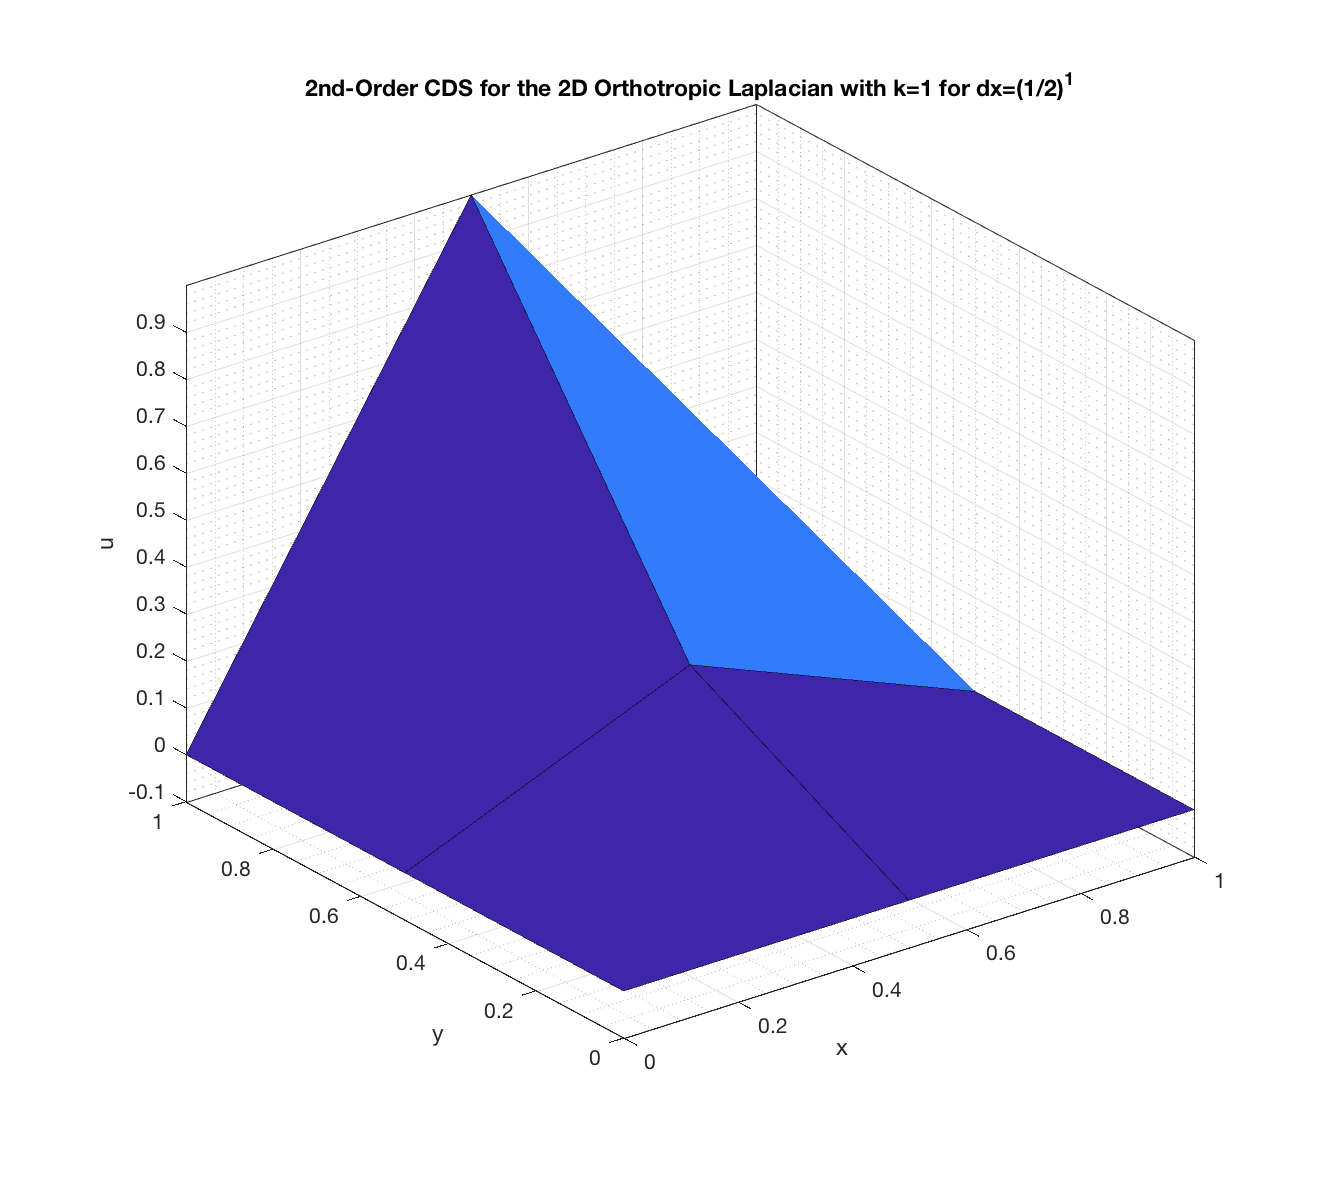
\includegraphics[width = 0.31\linewidth]{surface_order_2_k_1_dx_order_1}
		\includegraphics[width = 0.31\linewidth]{contour_order_2_k_1_dx_order_1}
		\caption{4th-Order CDS for the 2D Orthotropic Laplacian with $k = 1$ for $\Delta x = (1/2)^1$}
	\end{center}
\end{figure}

\begin{figure}[H]
	\begin{center}
		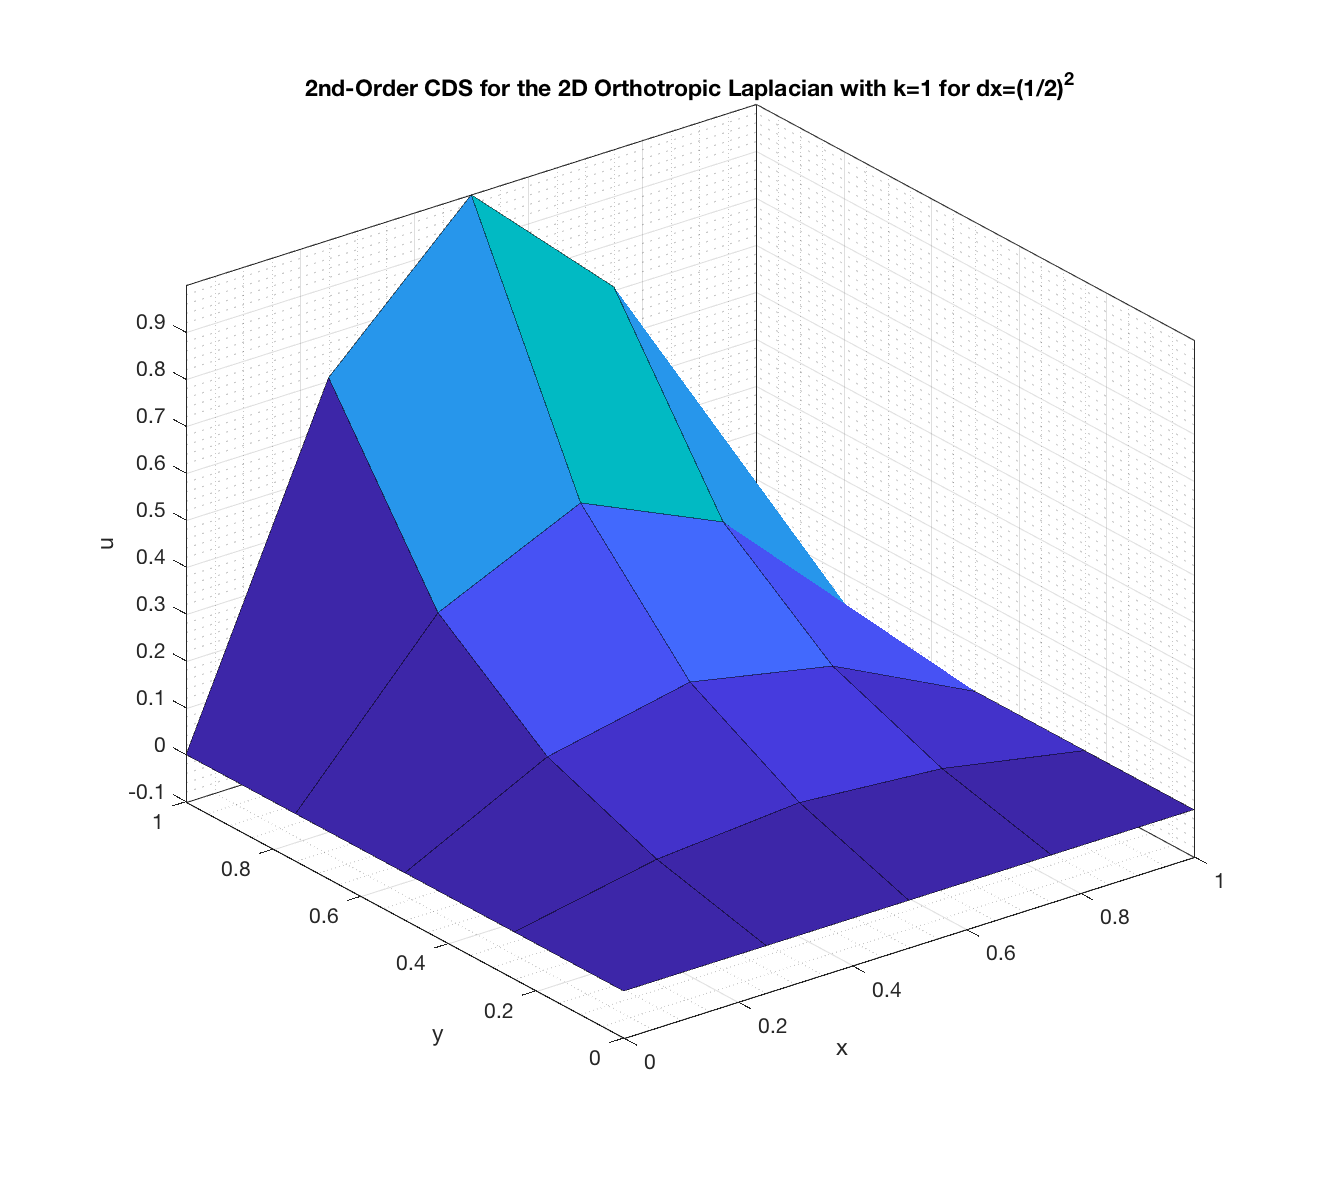
\includegraphics[width = 0.31\linewidth]{surface_order_2_k_1_dx_order_2}
		\includegraphics[width = 0.31\linewidth]{contour_order_2_k_1_dx_order_2}
		\caption{2nd-Order CDS for the 2D Orthotropic Laplacian with $k = 1$ for $\Delta x = (1/2)^2$}
	\end{center}
\end{figure}

\begin{figure}[H]
	\begin{center}
		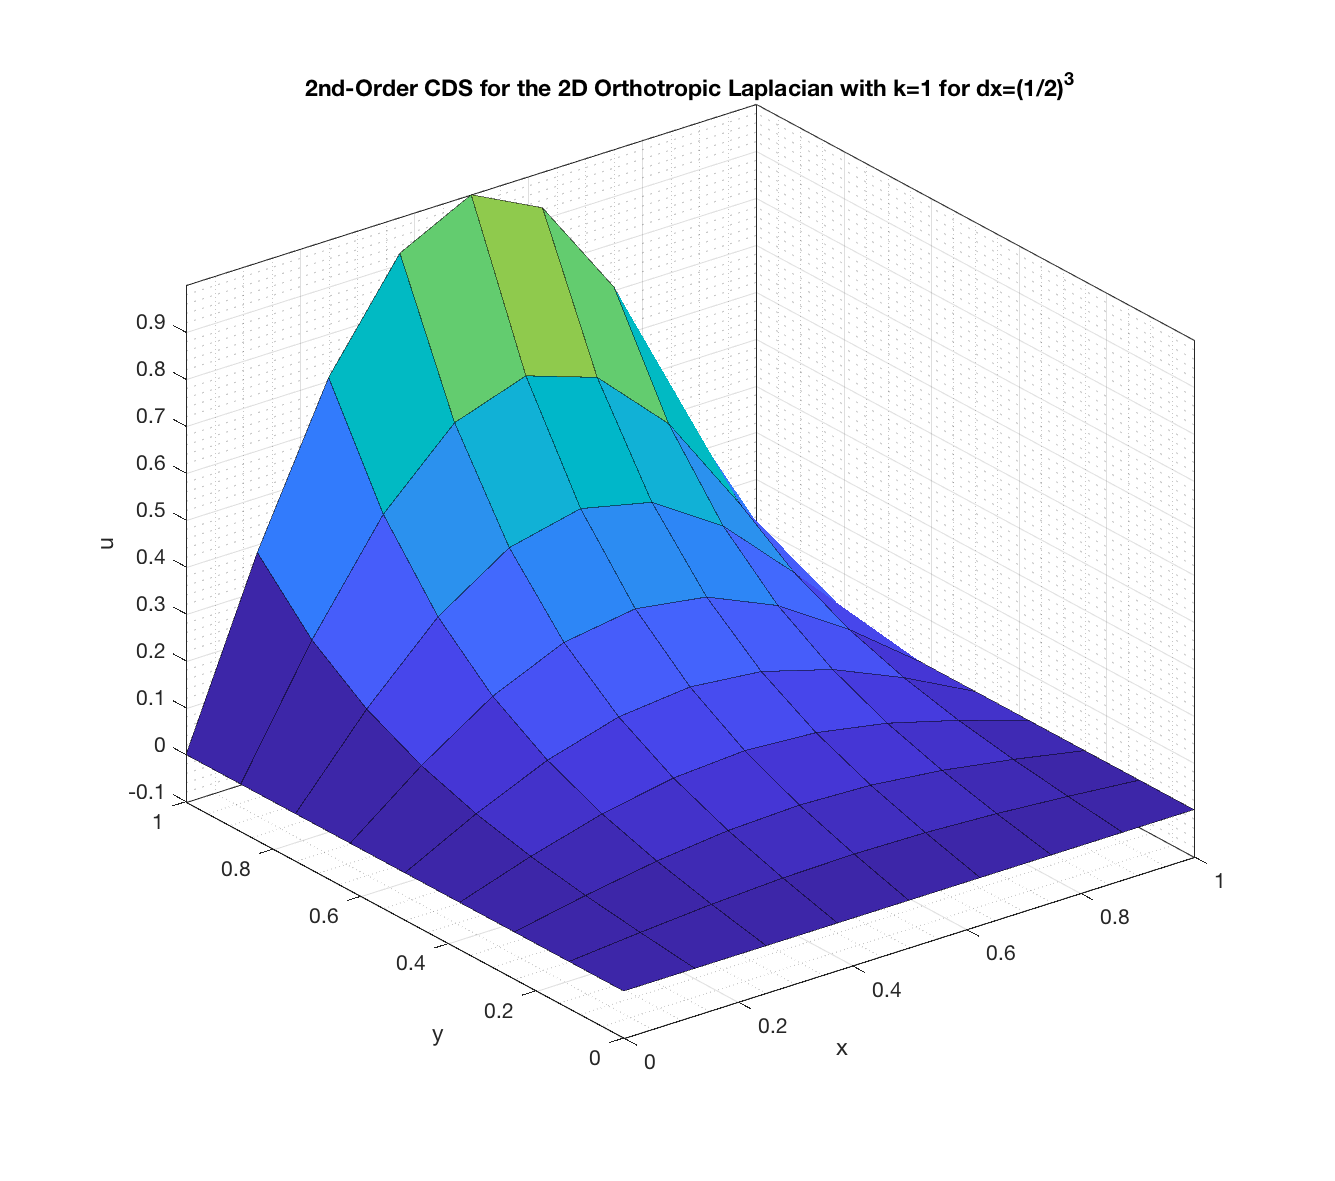
\includegraphics[width = 0.31\linewidth]{surface_order_2_k_1_dx_order_3}
		\includegraphics[width = 0.31\linewidth]{contour_order_2_k_1_dx_order_3}
		\caption{2nd-Order CDS for the 2D Orthotropic Laplacian with $k = 1$ for $\Delta x = (1/2)^3$}
	\end{center}
\end{figure}

\begin{figure}[H]
	\begin{center}
		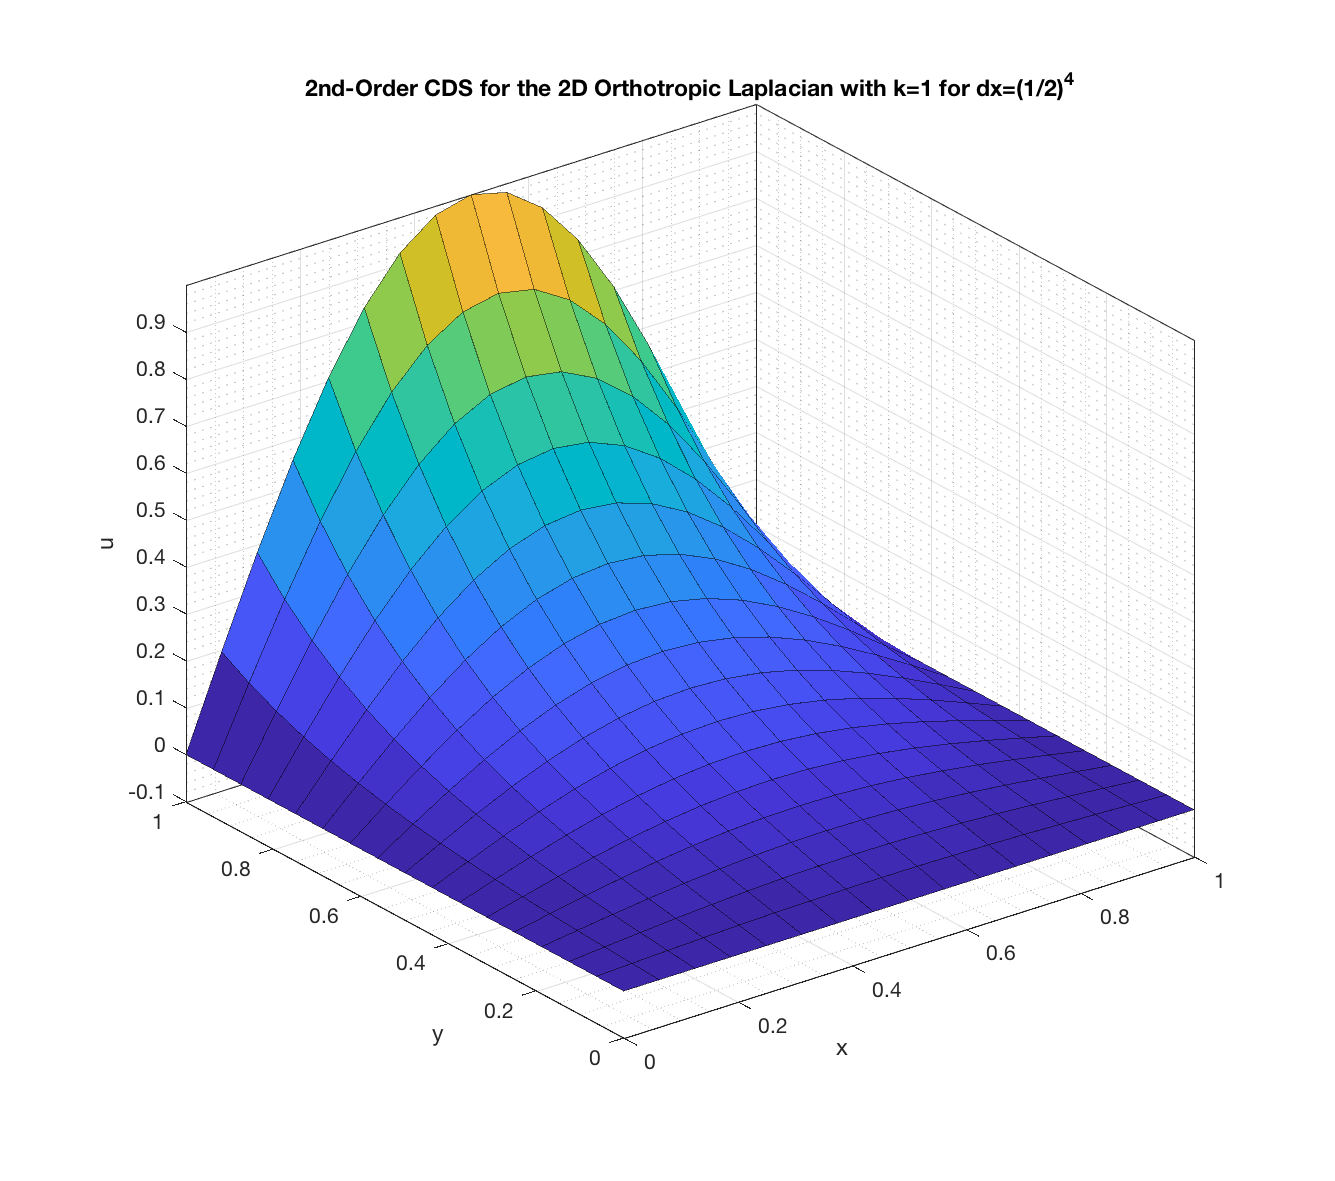
\includegraphics[width = 0.36\linewidth]{surface_order_2_k_1_dx_order_4}
		\includegraphics[width = 0.36\linewidth]{contour_order_2_k_1_dx_order_4}
		\caption{2nd-Order CDS for the 2D Orthotropic Laplacian with $k = 1$ for $\Delta x = (1/2)^4$}
	\end{center}
\end{figure}

\begin{figure}[H]
	\begin{center}
		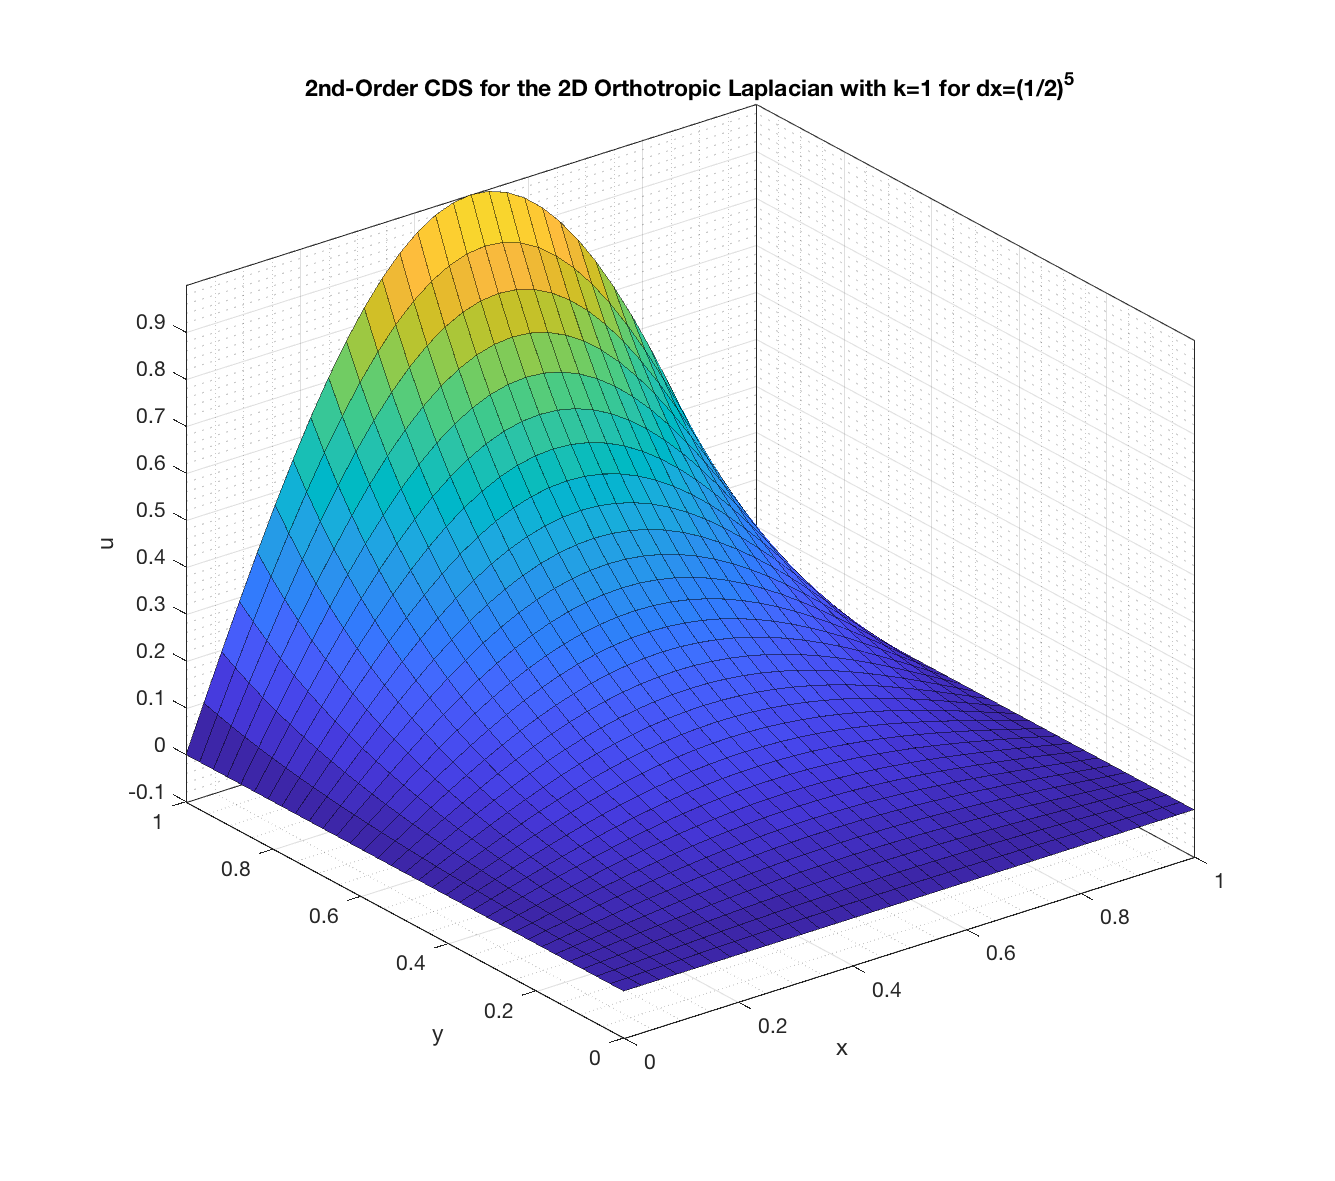
\includegraphics[width = 0.36\linewidth]{surface_order_2_k_1_dx_order_5}
		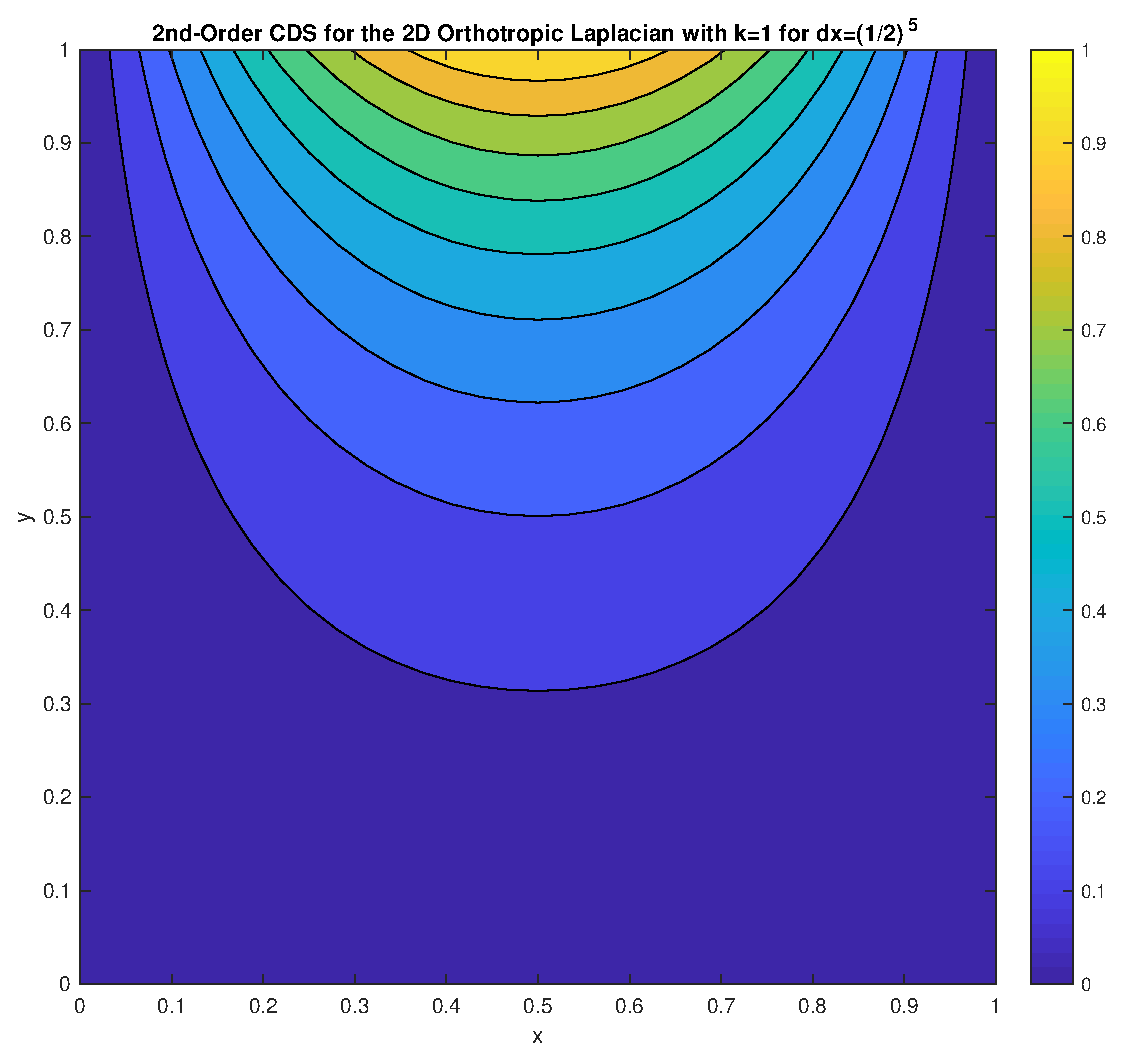
\includegraphics[width = 0.36\linewidth]{contour_order_2_k_1_dx_order_5}
		\caption{2nd-Order CDS for the 2D Orthotropic Laplacian with $k = 1$ for $\Delta x = (1/2)^5$}
	\end{center}
\end{figure}

\begin{figure}[H]
	\begin{center}
		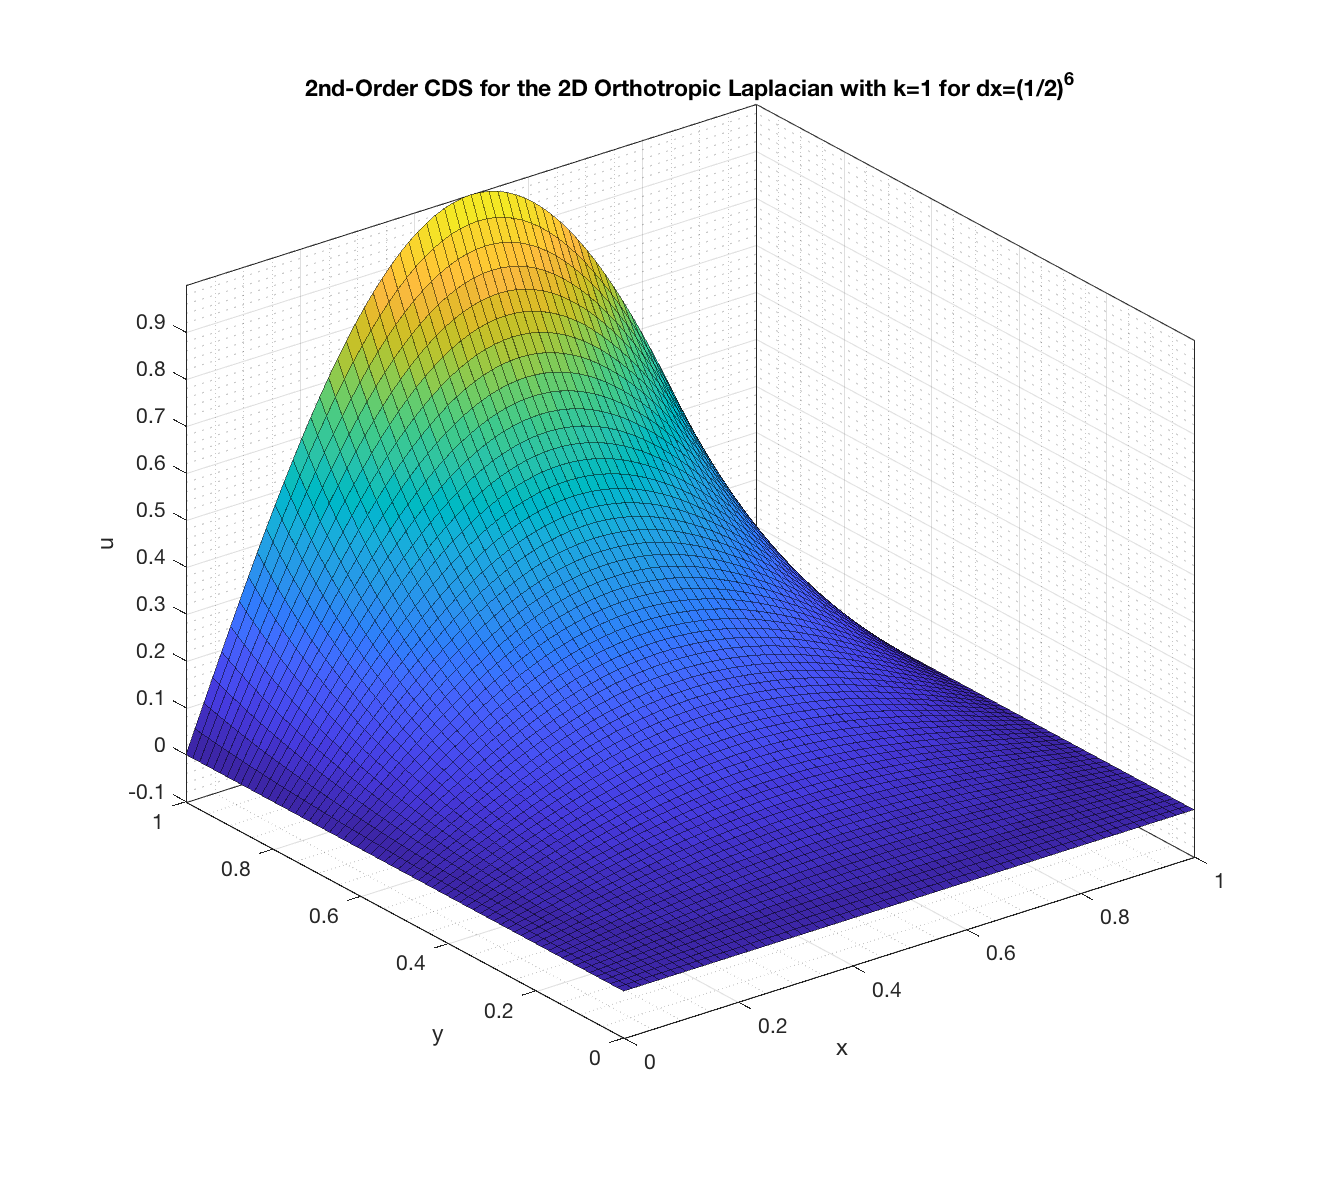
\includegraphics[width = 0.36\linewidth]{surface_order_2_k_1_dx_order_6}
		\includegraphics[width = 0.36\linewidth]{contour_order_2_k_1_dx_order_6}
		\caption{2nd-Order CDS for the 2D Orthotropic Laplacian with $k = 1$ for $\Delta x = (1/2)^6$}
	\end{center}
\end{figure}

\newpage

\begin{figure}[H]
	\begin{center}
		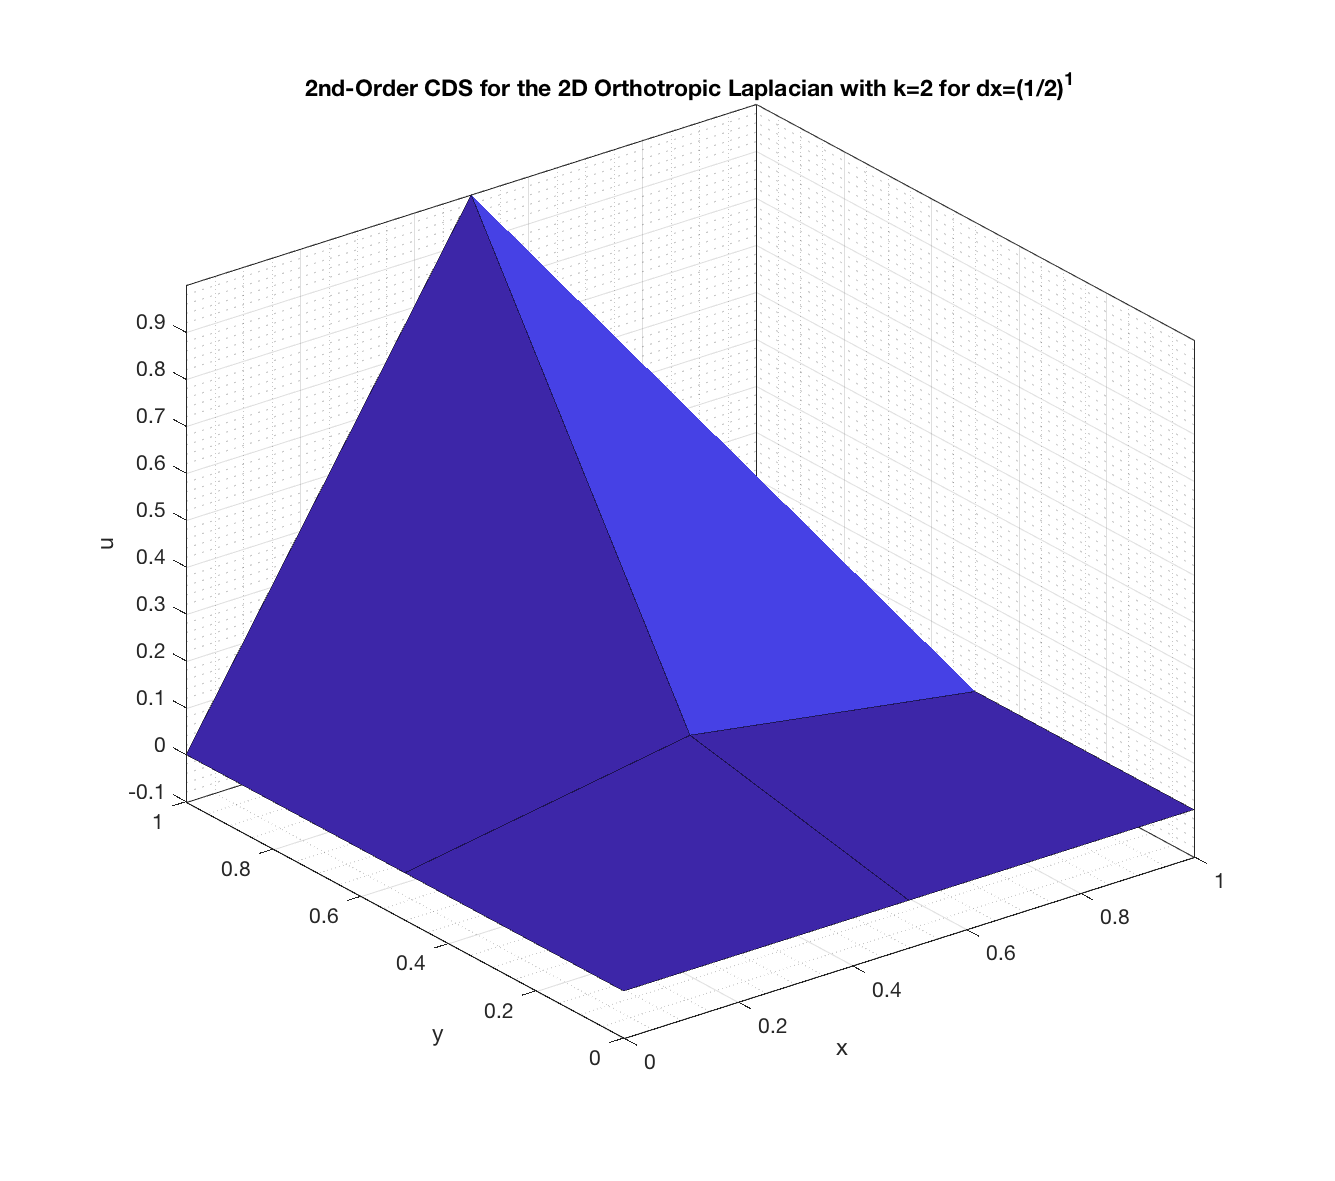
\includegraphics[width = 0.36\linewidth]{surface_order_2_k_2_dx_order_1}
		\includegraphics[width = 0.36\linewidth]{contour_order_2_k_2_dx_order_1}
		\caption{2nd-Order CDS for the 2D Orthotropic Laplacian with $k = 2$ for $\Delta x = (1/2)^1$}
	\end{center}
\end{figure}

\begin{figure}[H]
	\begin{center}
		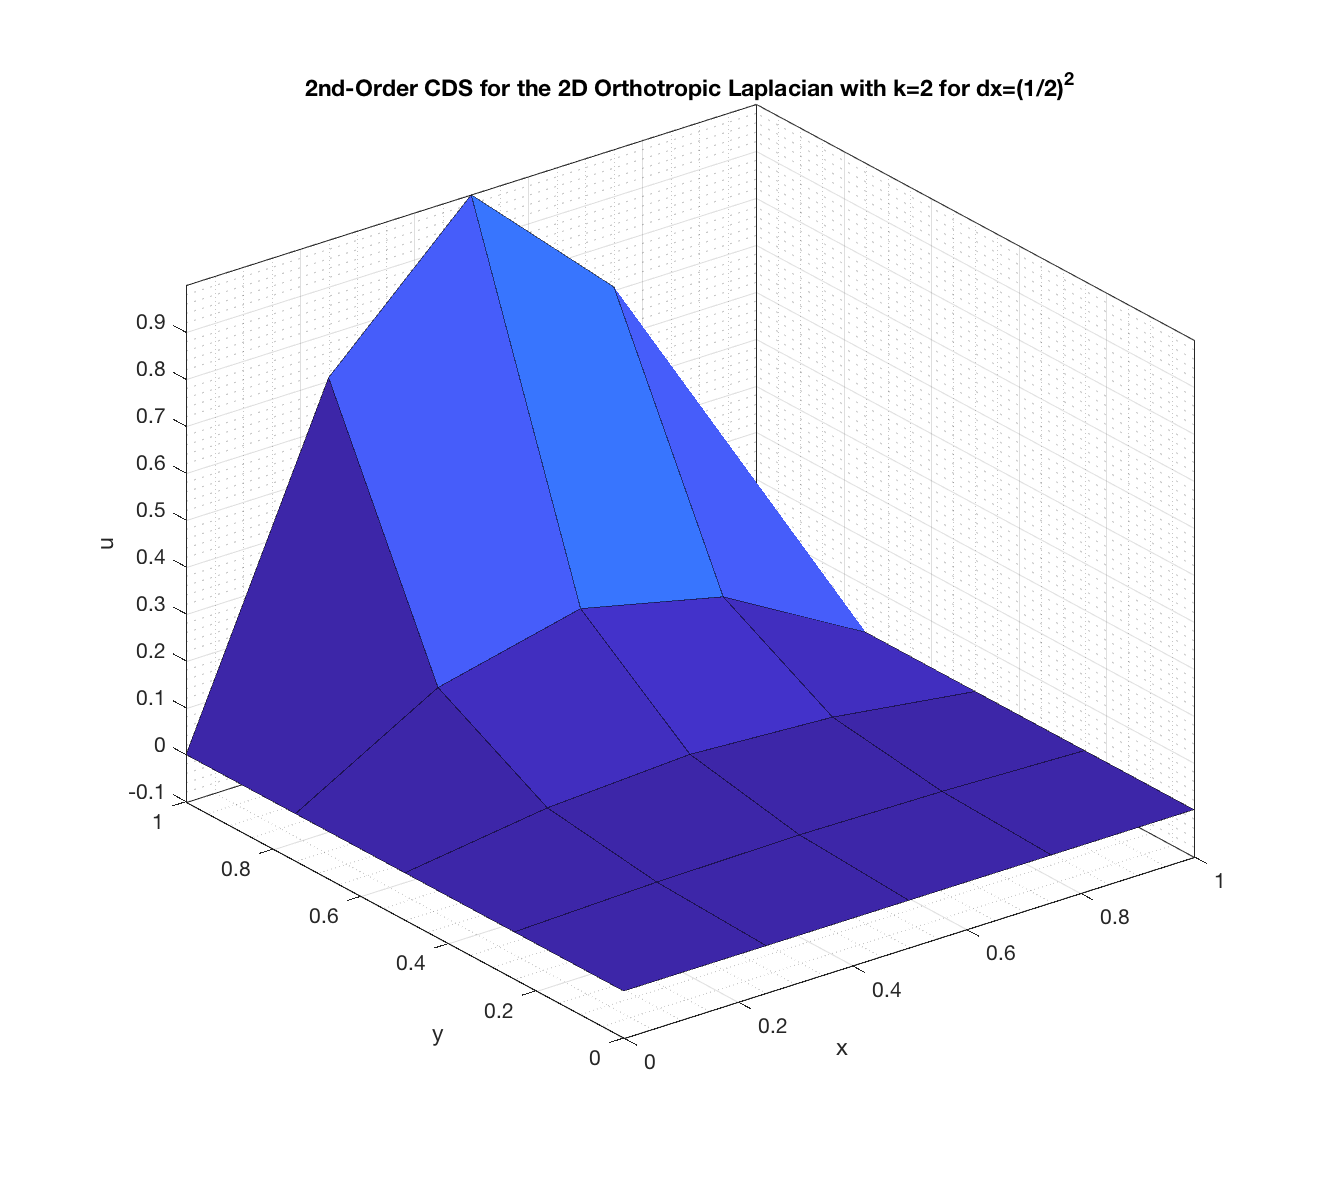
\includegraphics[width = 0.36\linewidth]{surface_order_2_k_2_dx_order_2}
		\includegraphics[width = 0.36\linewidth]{contour_order_2_k_2_dx_order_2}
		\caption{2nd-Order CDS for the 2D Orthotropic Laplacian with $k = 2$ for $\Delta x = (1/2)^2$}
	\end{center}
\end{figure}

\begin{figure}[H]
	\begin{center}
		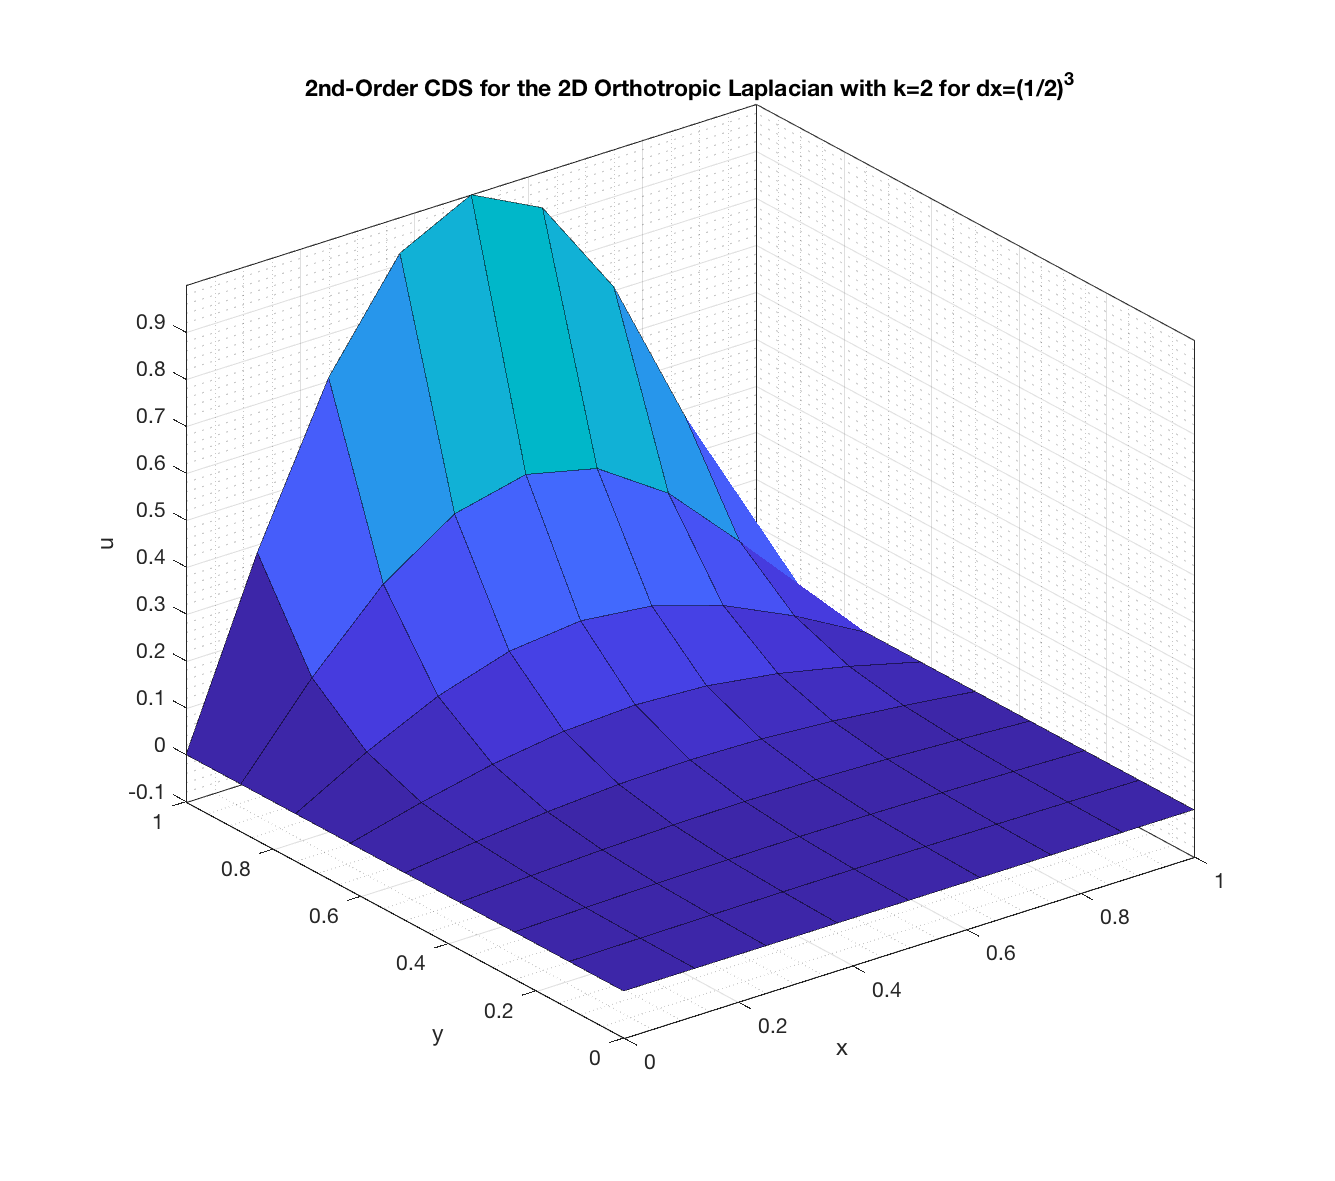
\includegraphics[width = 0.36\linewidth]{surface_order_2_k_2_dx_order_3}
		\includegraphics[width = 0.36\linewidth]{contour_order_2_k_2_dx_order_3}
		\caption{2nd-Order CDS for the 2D Orthotropic Laplacian with $k = 2$ for $\Delta x = (1/2)^3$}
	\end{center}
\end{figure}

\begin{figure}[H]
	\begin{center}
		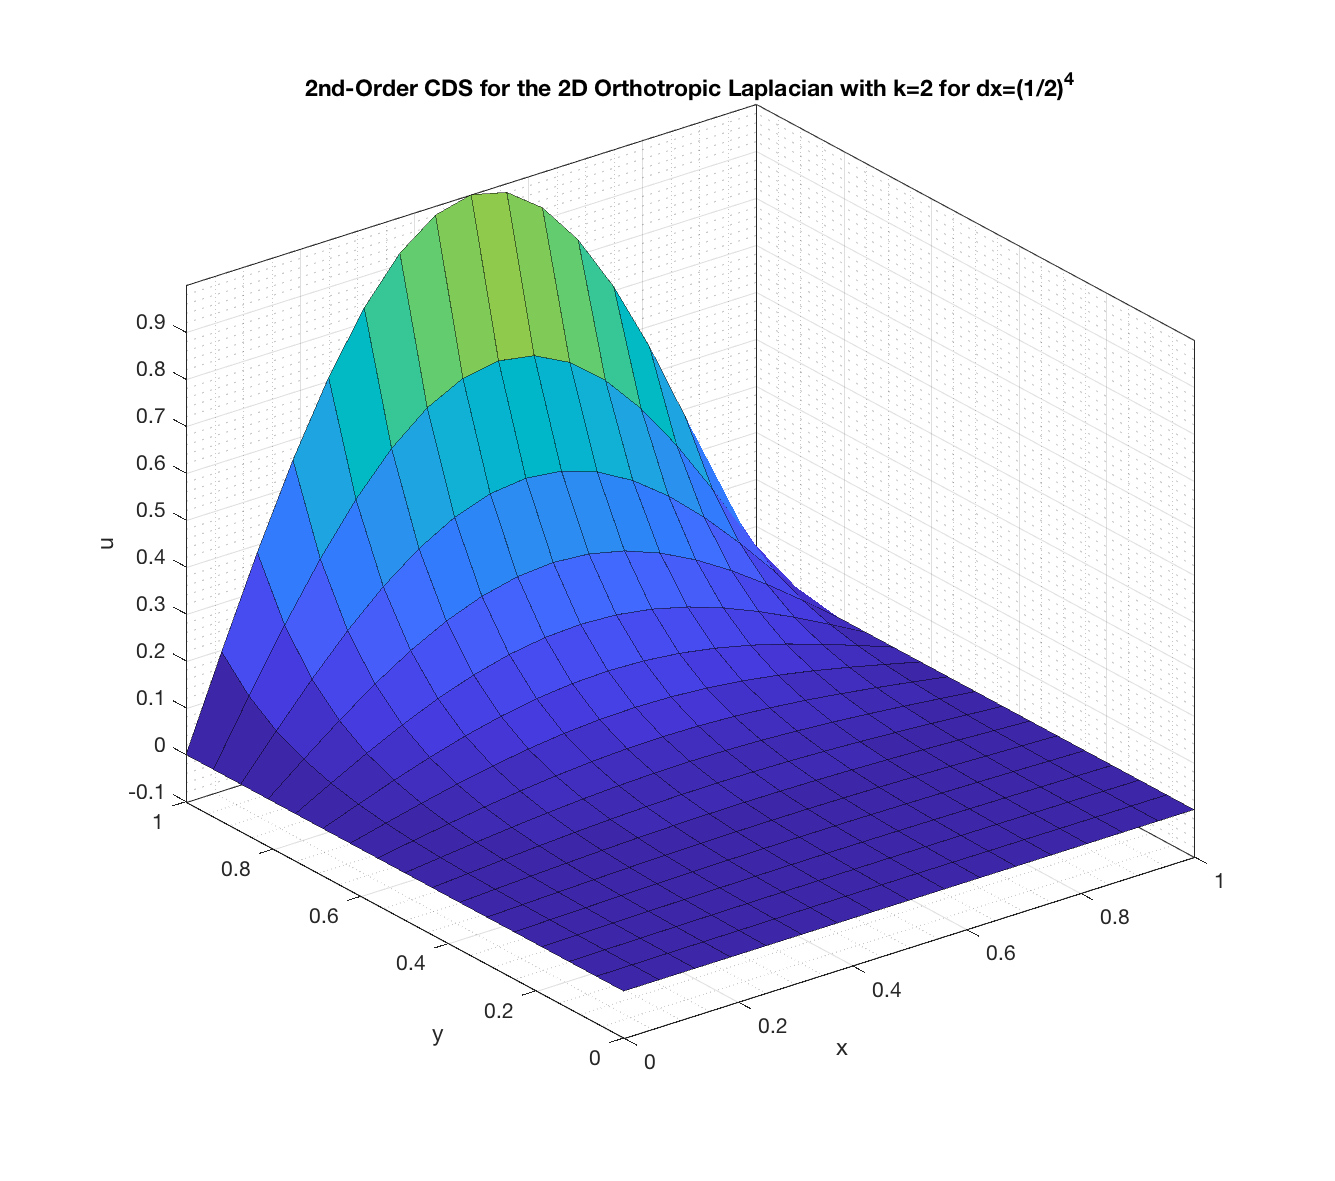
\includegraphics[width = 0.36\linewidth]{surface_order_2_k_2_dx_order_4}
		\includegraphics[width = 0.36\linewidth]{contour_order_2_k_2_dx_order_4}
		\caption{2nd-Order CDS for the 2D Orthotropic Laplacian with $k = 2$ for $\Delta x = (1/2)^4$}
	\end{center}
\end{figure}

\begin{figure}[H]
	\begin{center}
		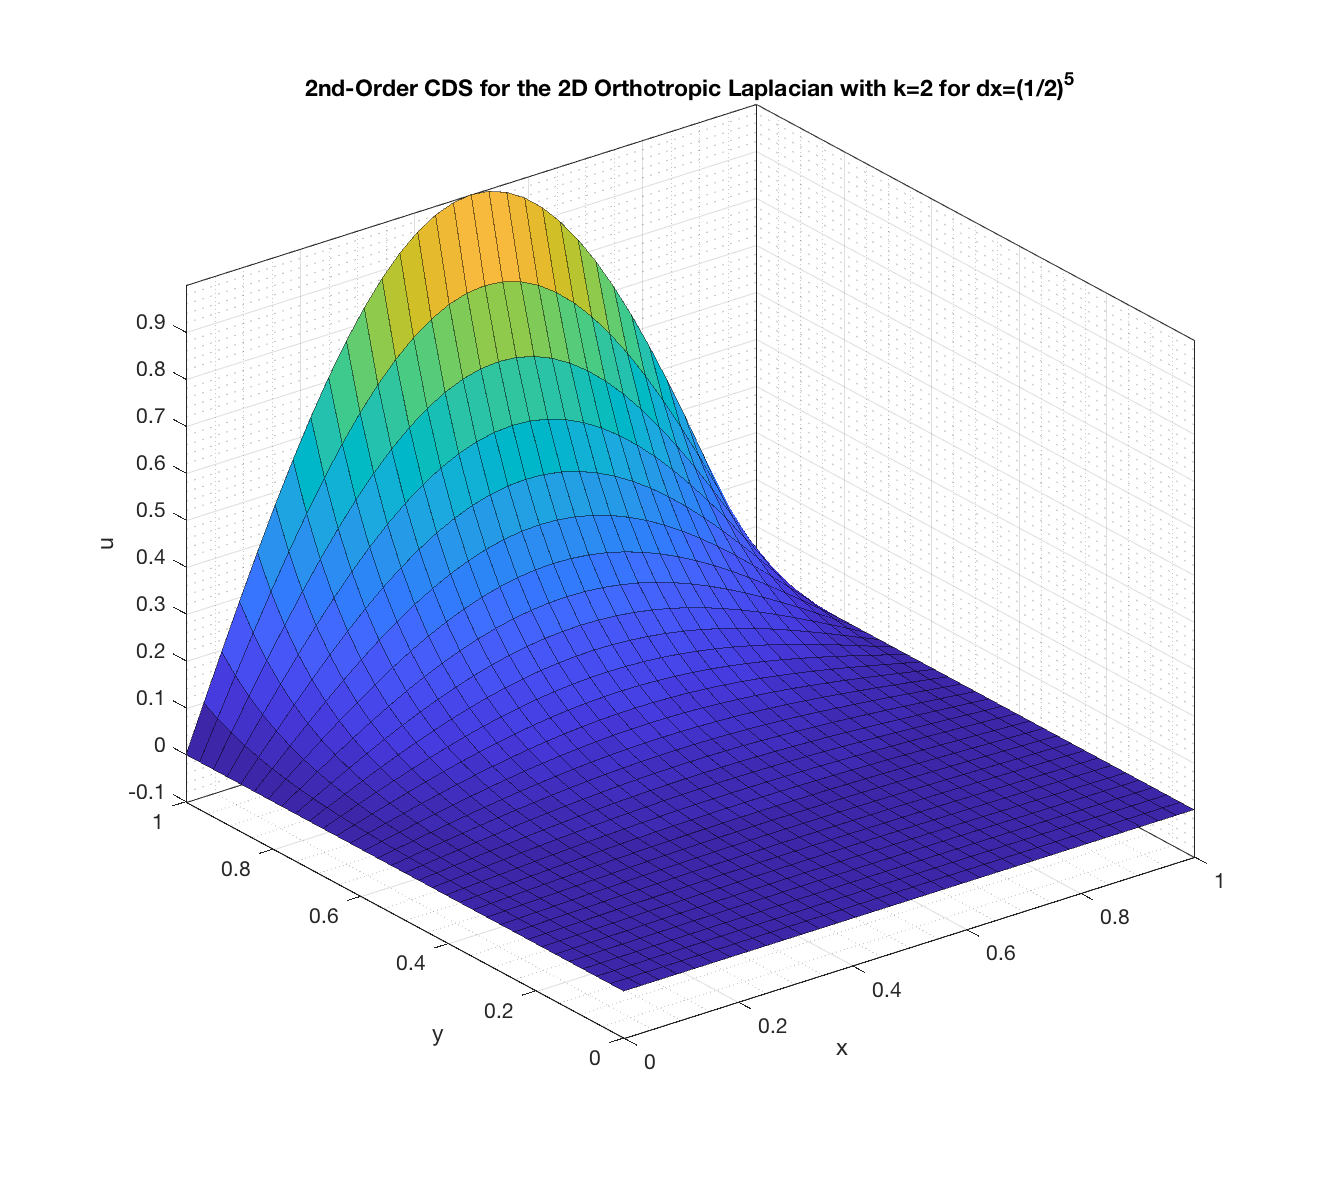
\includegraphics[width = 0.36\linewidth]{surface_order_2_k_2_dx_order_5}
		\includegraphics[width = 0.36\linewidth]{contour_order_2_k_2_dx_order_5}
		\caption{2nd-Order CDS for the 2D Orthotropic Laplacian with $k = 2$ for $\Delta x = (1/2)^5$}
	\end{center}
\end{figure}

\begin{figure}[H]
	\begin{center}
		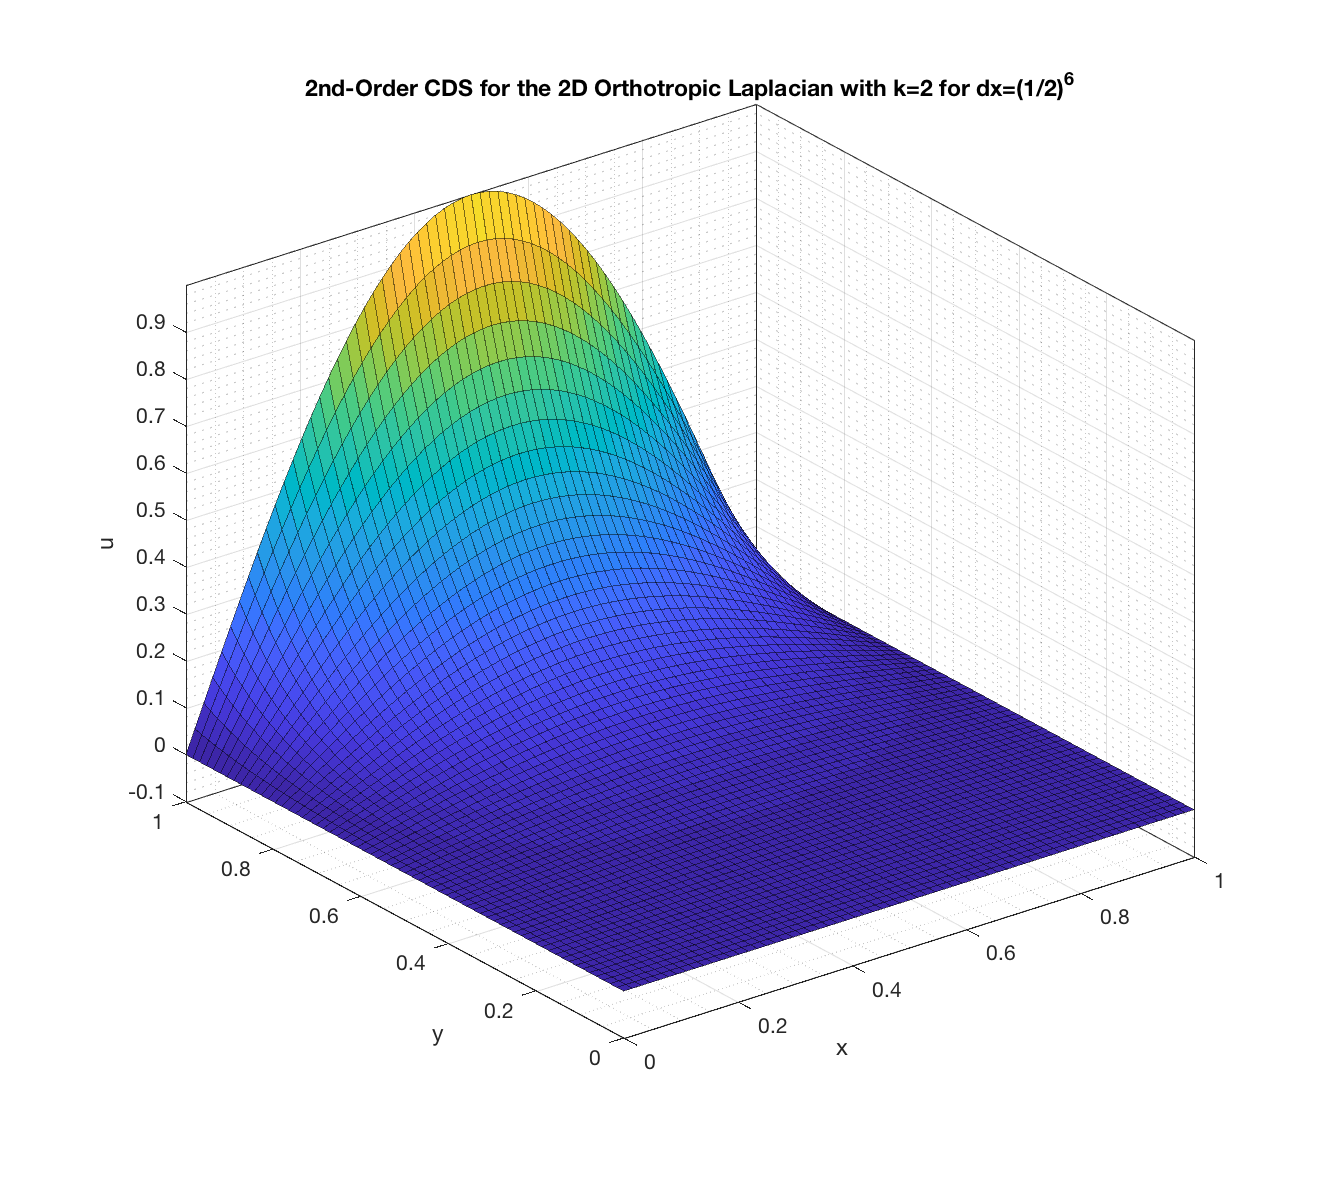
\includegraphics[width = 0.36\linewidth]{surface_order_2_k_2_dx_order_6}
		\includegraphics[width = 0.36\linewidth]{contour_order_2_k_2_dx_order_6}
		\caption{2nd-Order CDS for the 2D Orthotropic Laplacian with $k = 2$ for $\Delta x = (1/2)^6$}
	\end{center}
\end{figure}

\newpage

\begin{figure}[H]
	\begin{center}
		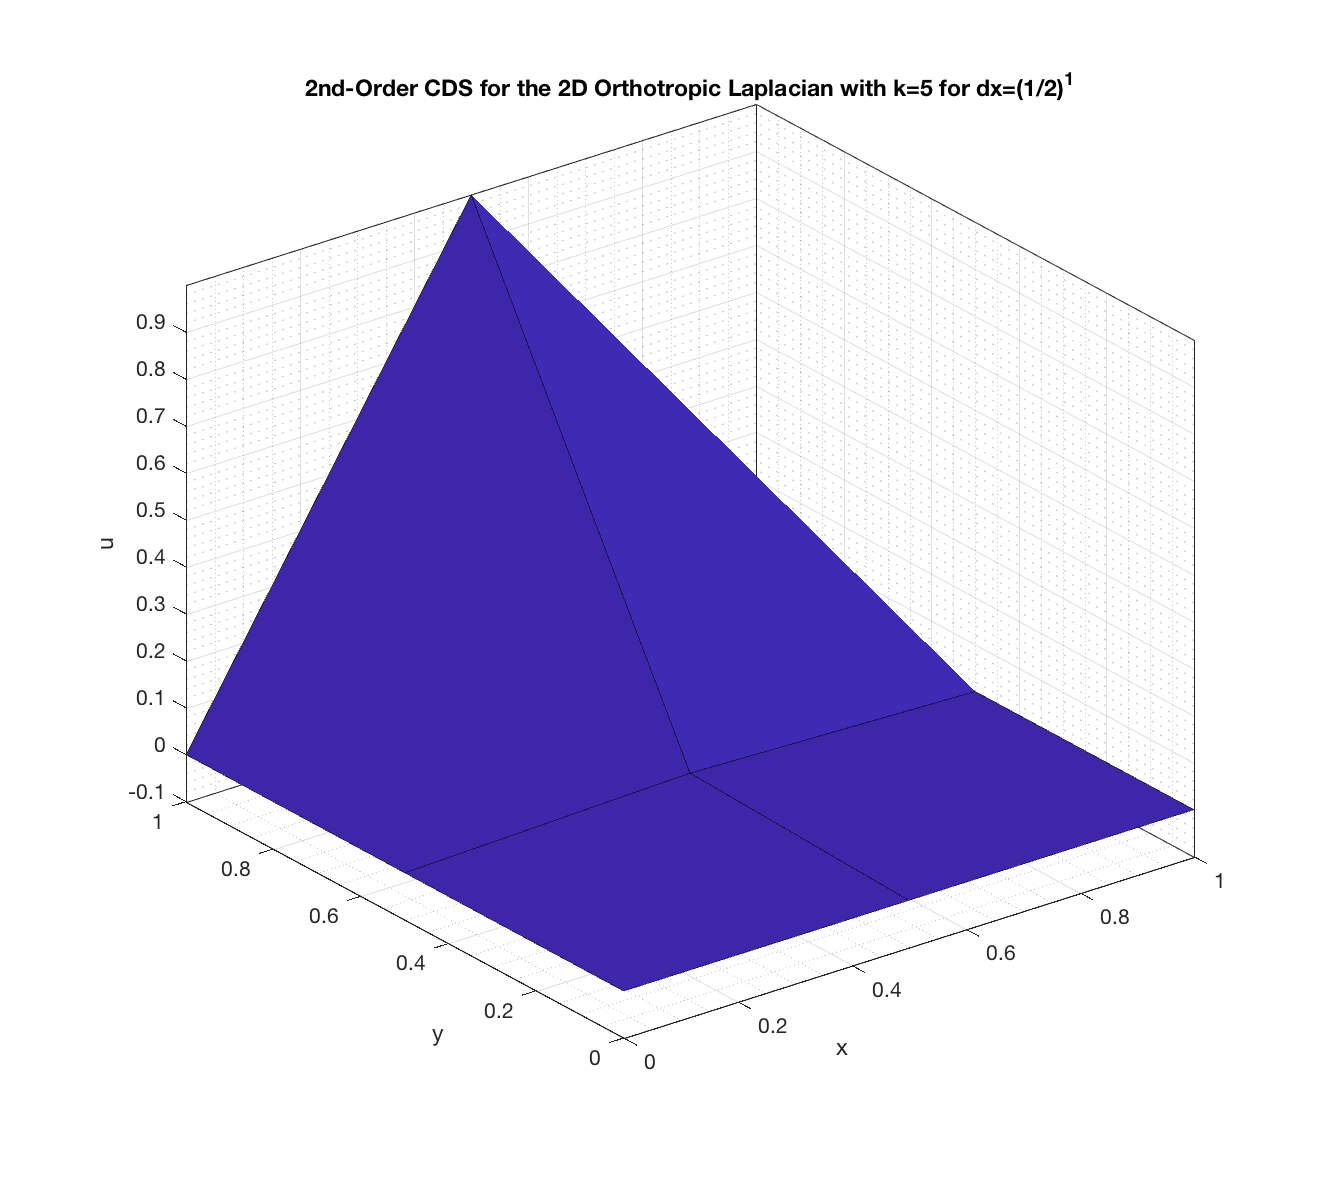
\includegraphics[width = 0.36\linewidth]{surface_order_2_k_5_dx_order_1}
		\includegraphics[width = 0.36\linewidth]{contour_order_2_k_5_dx_order_1}
		\caption{2nd-Order CDS for the 2D Orthotropic Laplacian with $k = 5$ for $\Delta x = (1/2)^1$}
	\end{center}
\end{figure}

\begin{figure}[H]
	\begin{center}
		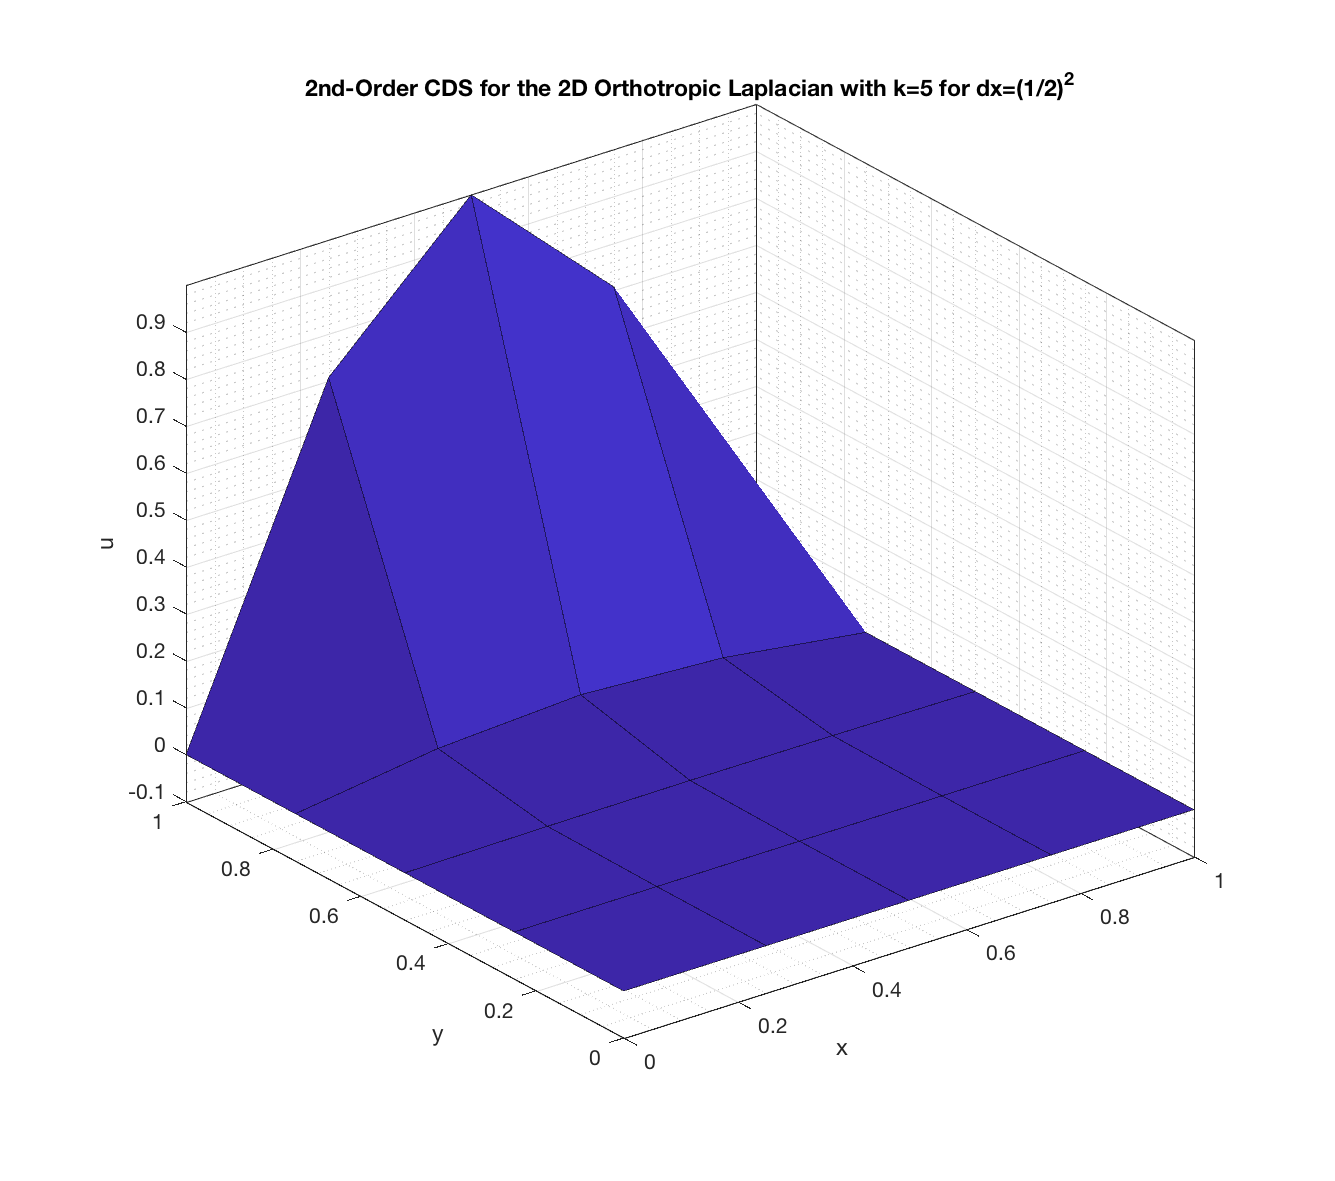
\includegraphics[width = 0.36\linewidth]{surface_order_2_k_5_dx_order_2}
		\includegraphics[width = 0.36\linewidth]{contour_order_2_k_5_dx_order_2}
		\caption{2nd-Order CDS for the 2D Orthotropic Laplacian with $k = 5$ for $\Delta x = (1/2)^2$}
	\end{center}
\end{figure}

\begin{figure}[H]
	\begin{center}
		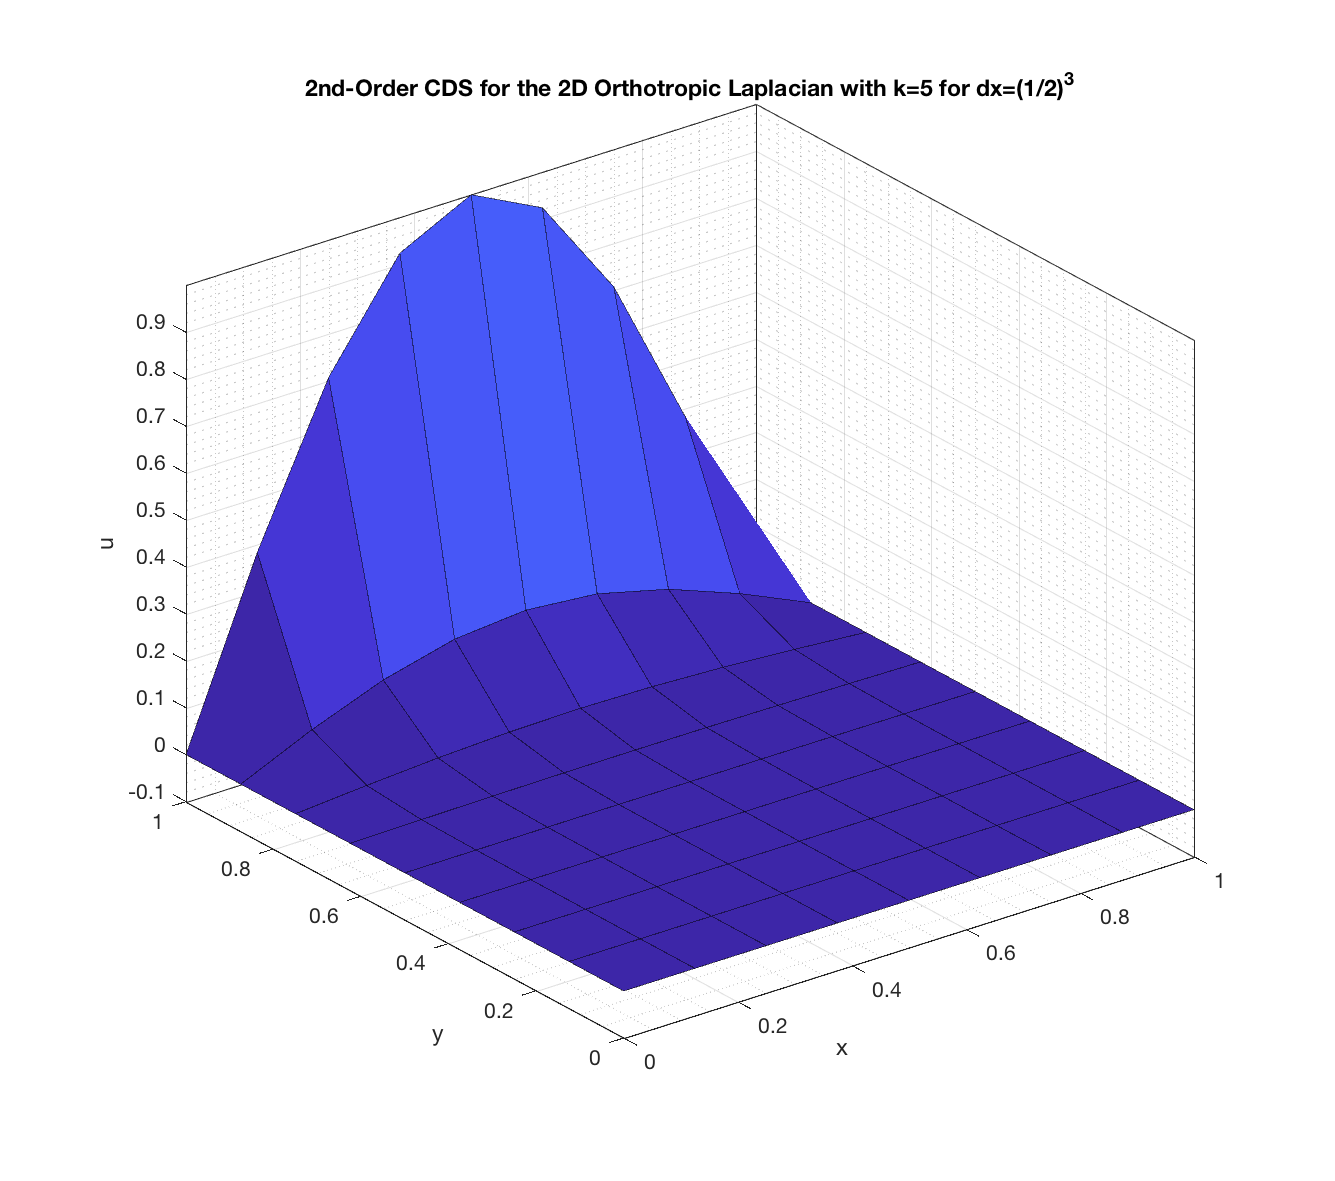
\includegraphics[width = 0.36\linewidth]{surface_order_2_k_5_dx_order_3}
		\includegraphics[width = 0.36\linewidth]{contour_order_2_k_5_dx_order_3}
		\caption{2nd-Order CDS for the 2D Orthotropic Laplacian with $k = 5$ for $\Delta x = (1/2)^3$}
	\end{center}
\end{figure}

\begin{figure}[H]
	\begin{center}
		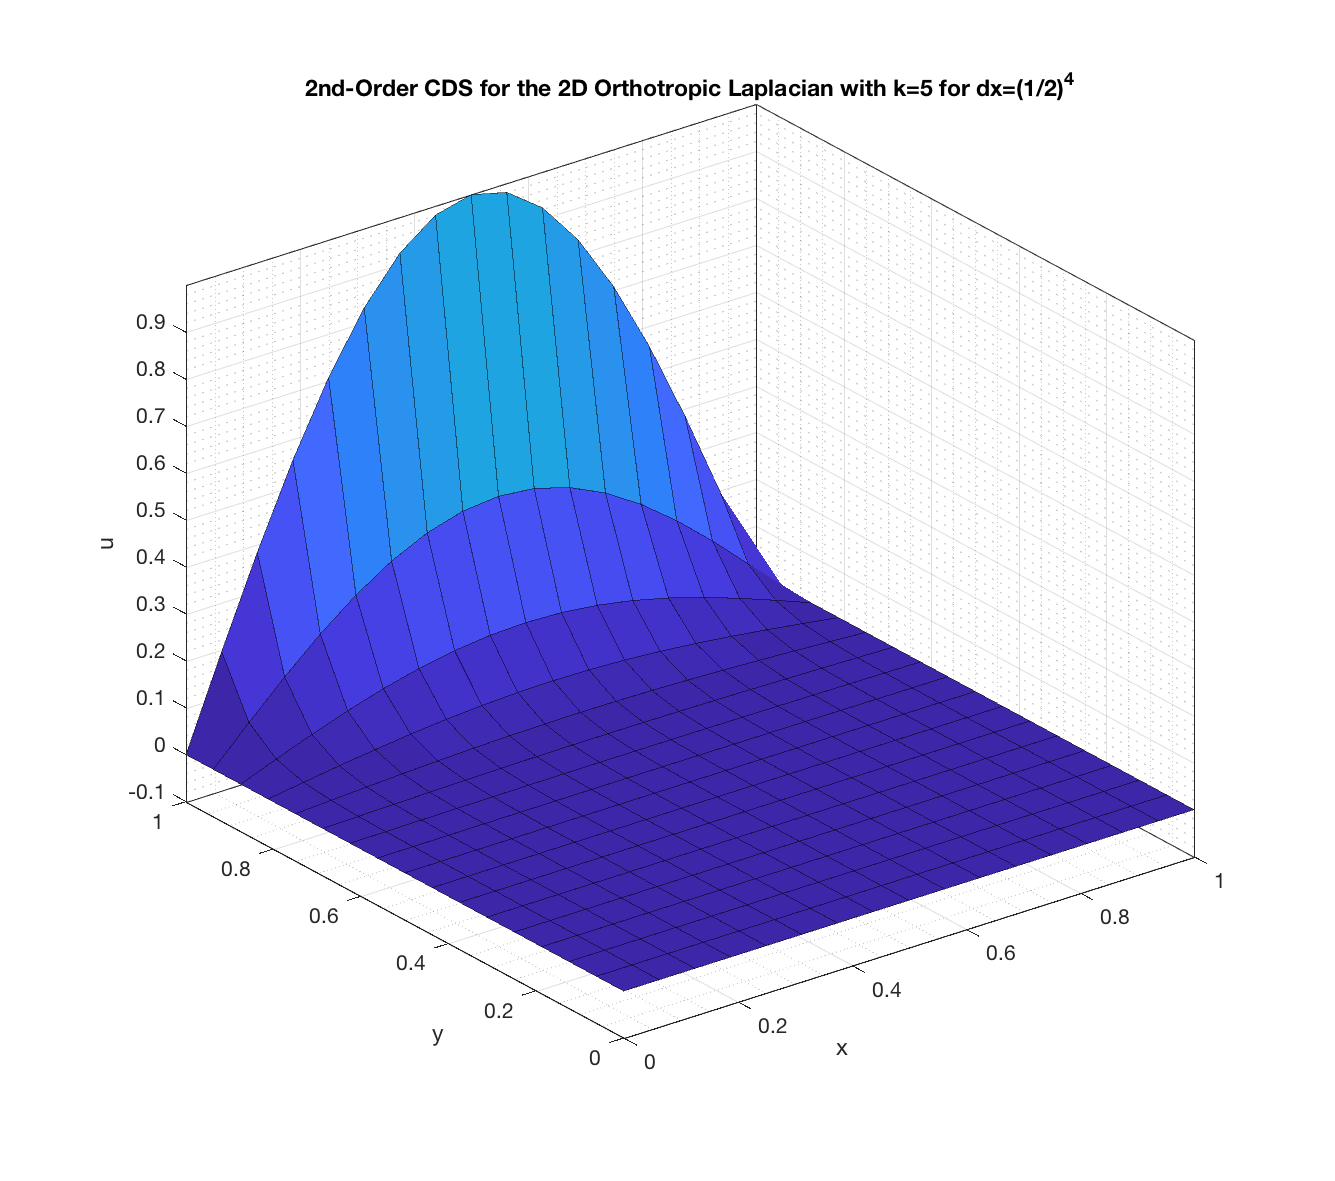
\includegraphics[width = 0.36\linewidth]{surface_order_2_k_5_dx_order_4}
		\includegraphics[width = 0.36\linewidth]{contour_order_2_k_5_dx_order_4}
		\caption{2nd-Order CDS for the 2D Orthotropic Laplacian with $k = 5$ for $\Delta x = (1/2)^4$}
	\end{center}
\end{figure}

\begin{figure}[H]
	\begin{center}
		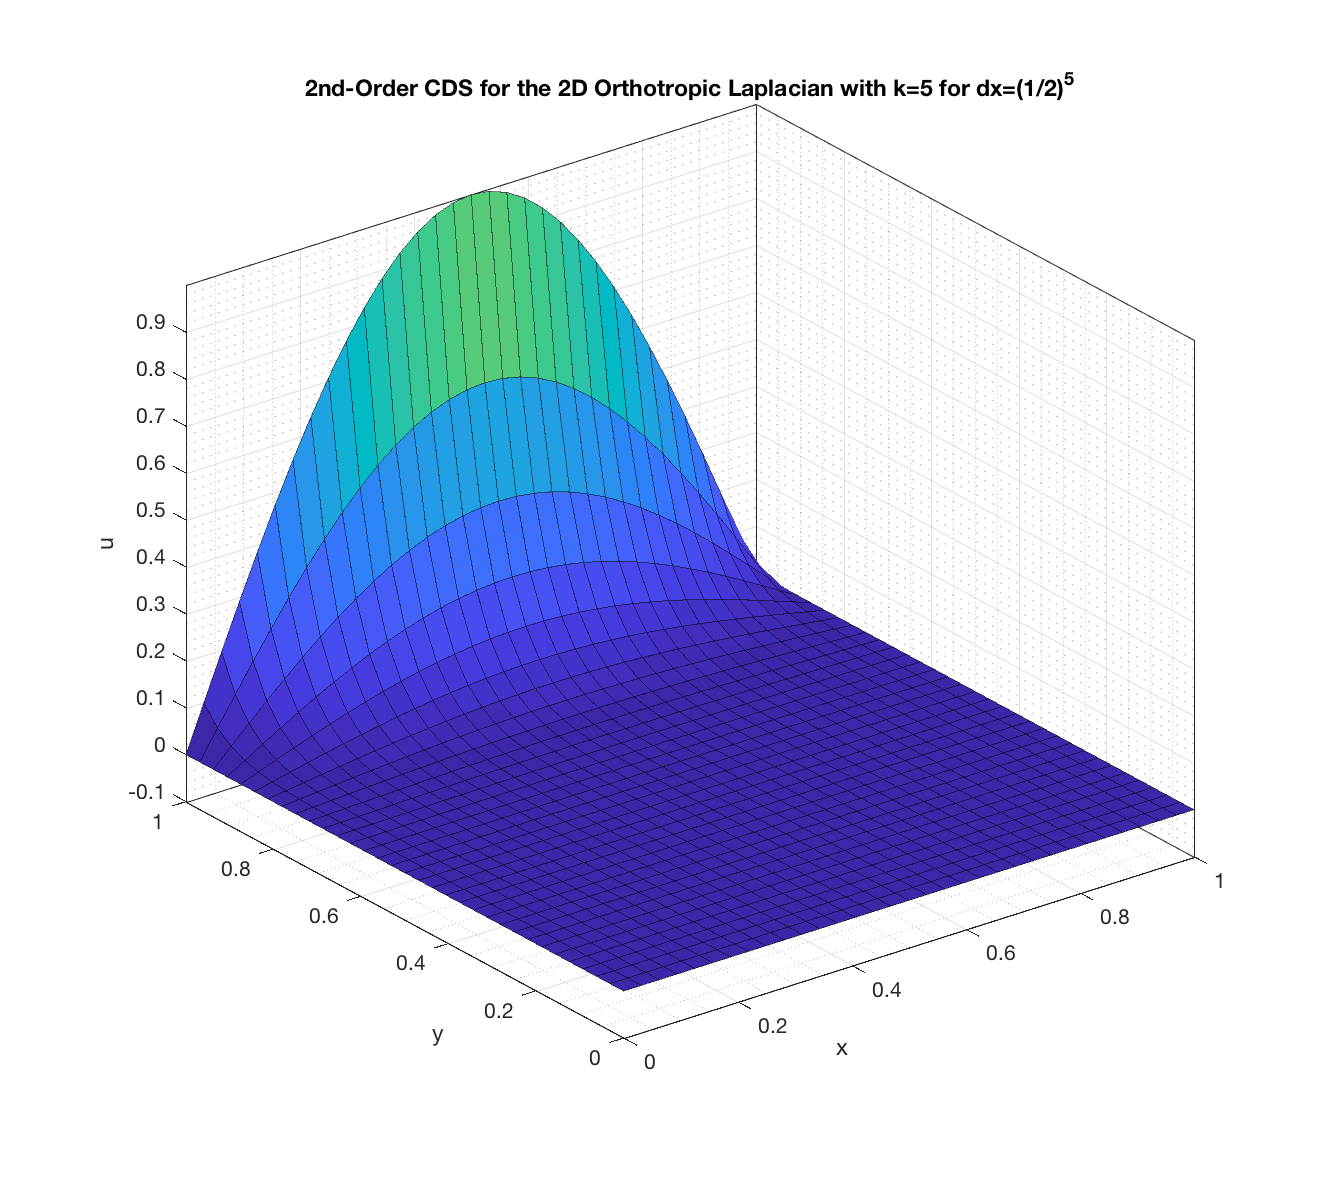
\includegraphics[width = 0.36\linewidth]{surface_order_2_k_5_dx_order_5}
		\includegraphics[width = 0.36\linewidth]{contour_order_2_k_5_dx_order_5}
		\caption{2nd-Order CDS for the 2D Orthotropic Laplacian with $k = 5$ for $\Delta x = (1/2)^5$}
	\end{center}
\end{figure}

\begin{figure}[H]
	\begin{center}
		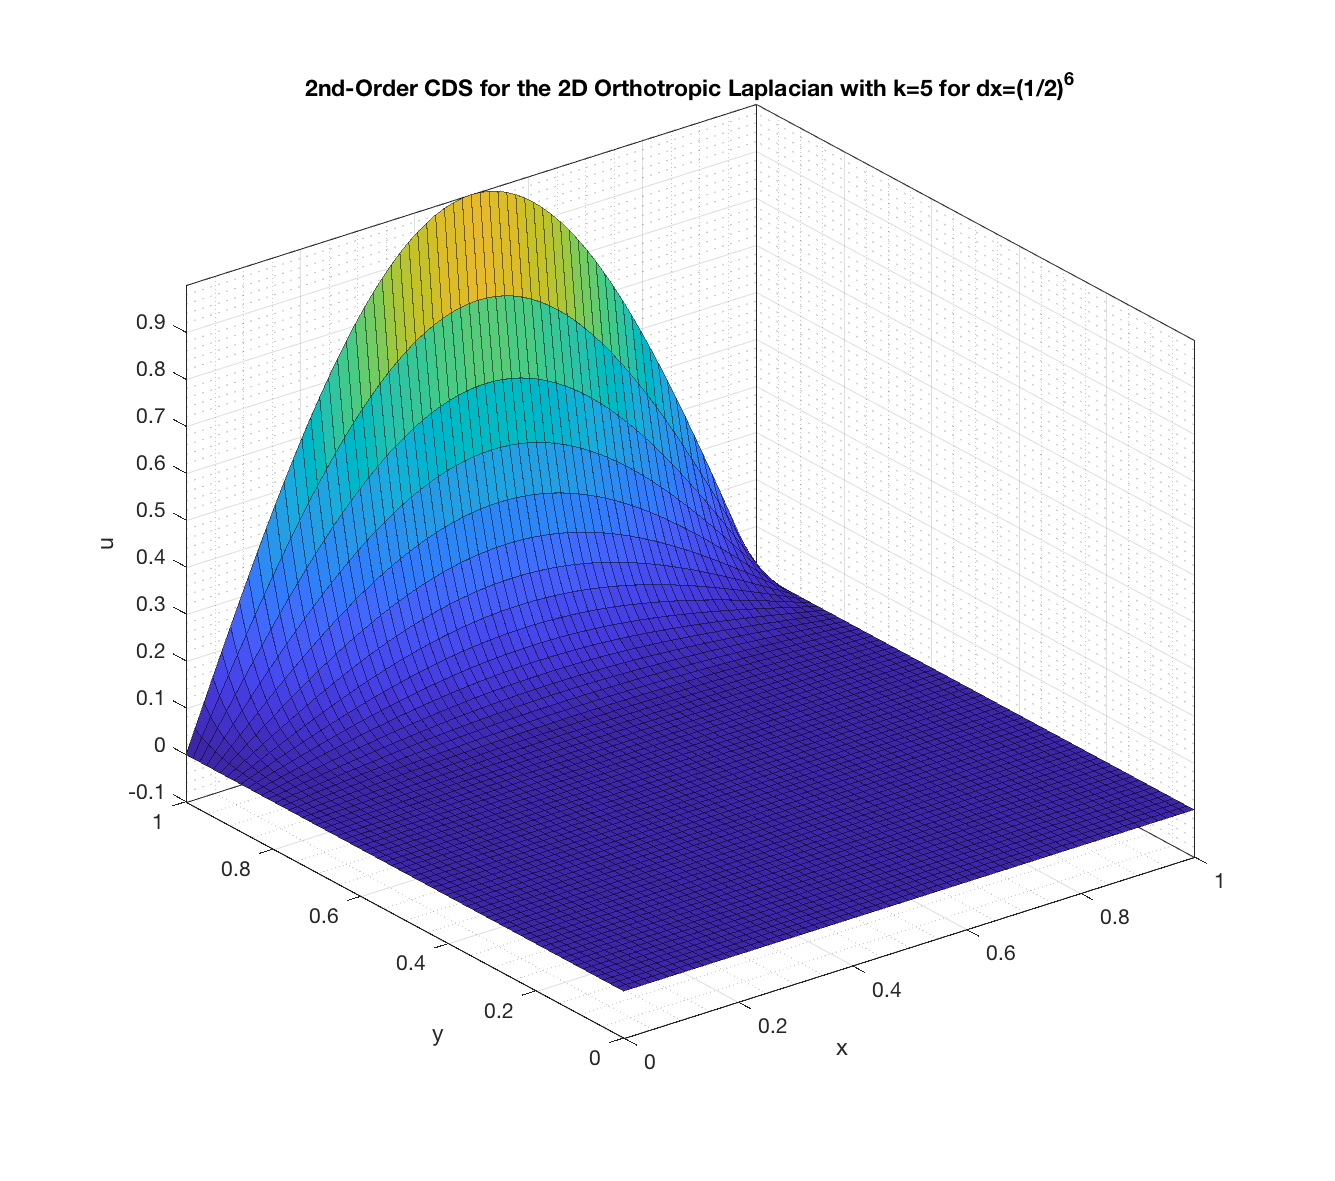
\includegraphics[width = 0.36\linewidth]{surface_order_2_k_5_dx_order_6}
		\includegraphics[width = 0.36\linewidth]{contour_order_2_k_5_dx_order_6}
		\caption{2nd-Order CDS for the 2D Orthotropic Laplacian with $k = 5$ for $\Delta x = (1/2)^6$}
	\end{center}
\end{figure}

\newpage

\begin{figure}[H]
	\begin{center}
		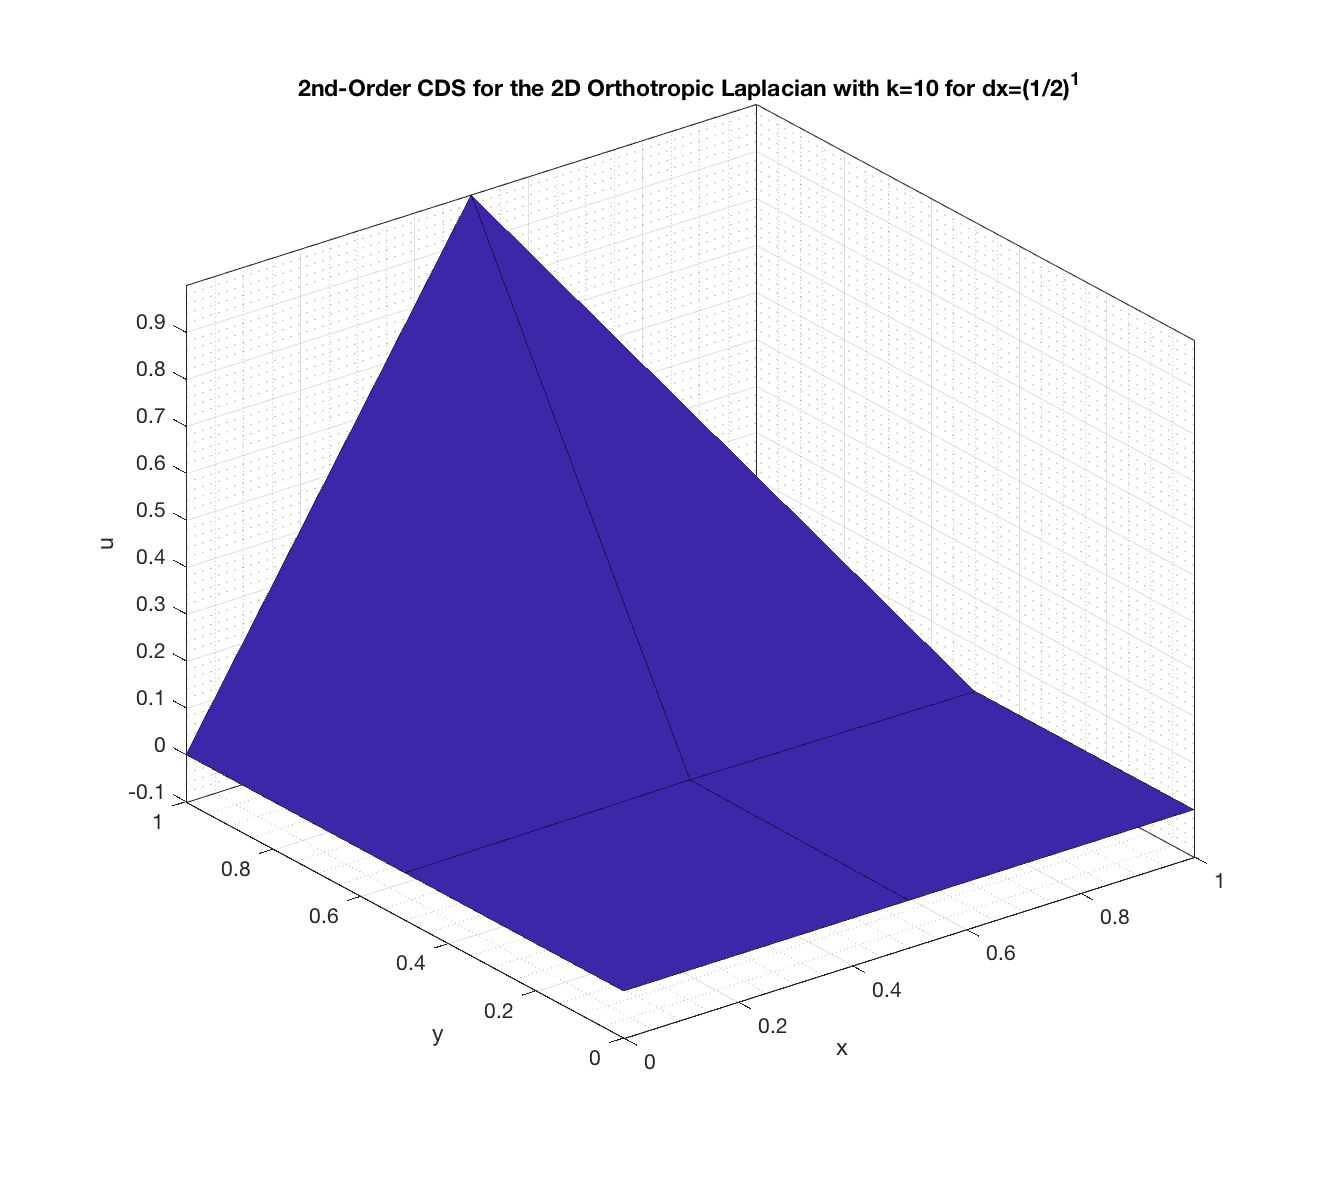
\includegraphics[width = 0.36\linewidth]{surface_order_2_k_10_dx_order_1}
		\includegraphics[width = 0.36\linewidth]{contour_order_2_k_10_dx_order_1}
		\caption{2nd-Order CDS for the 2D Orthotropic Laplacian with $k = 10$ for $\Delta x = (1/2)^1$}
	\end{center}
\end{figure}

\begin{figure}[H]
	\begin{center}
		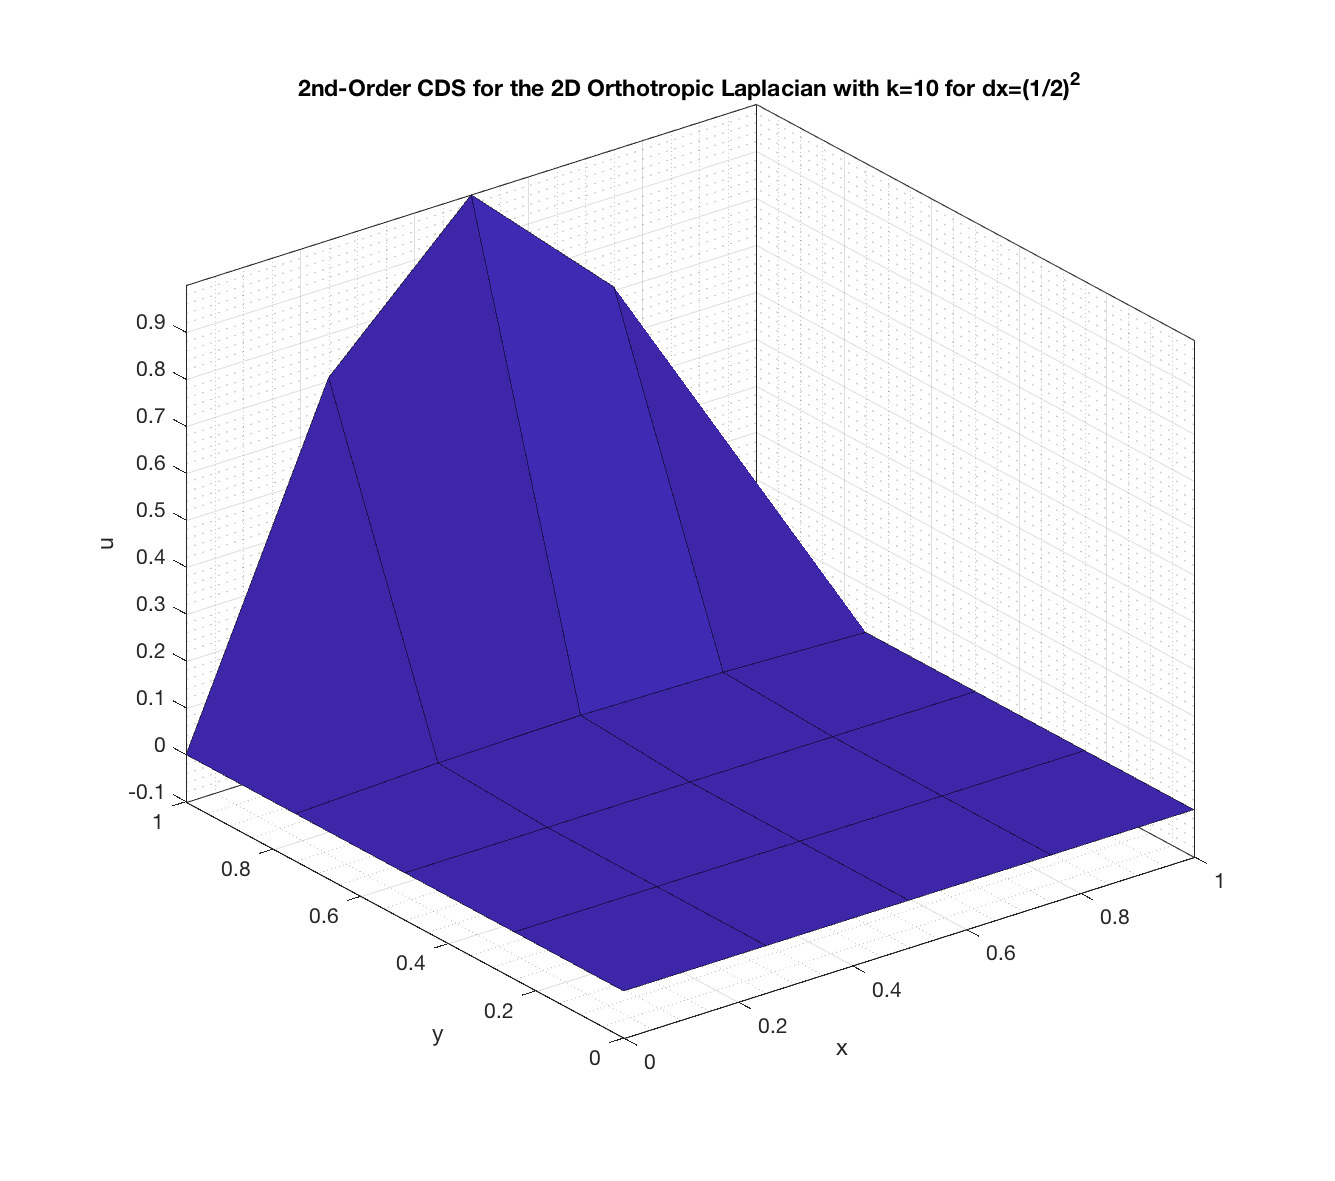
\includegraphics[width = 0.36\linewidth]{surface_order_2_k_10_dx_order_2}
		\includegraphics[width = 0.36\linewidth]{contour_order_2_k_10_dx_order_2}
		\caption{2nd-Order CDS for the 2D Orthotropic Laplacian with $k = 10$ for $\Delta x = (1/2)^2$}
	\end{center}
\end{figure}

\begin{figure}[H]
	\begin{center}
		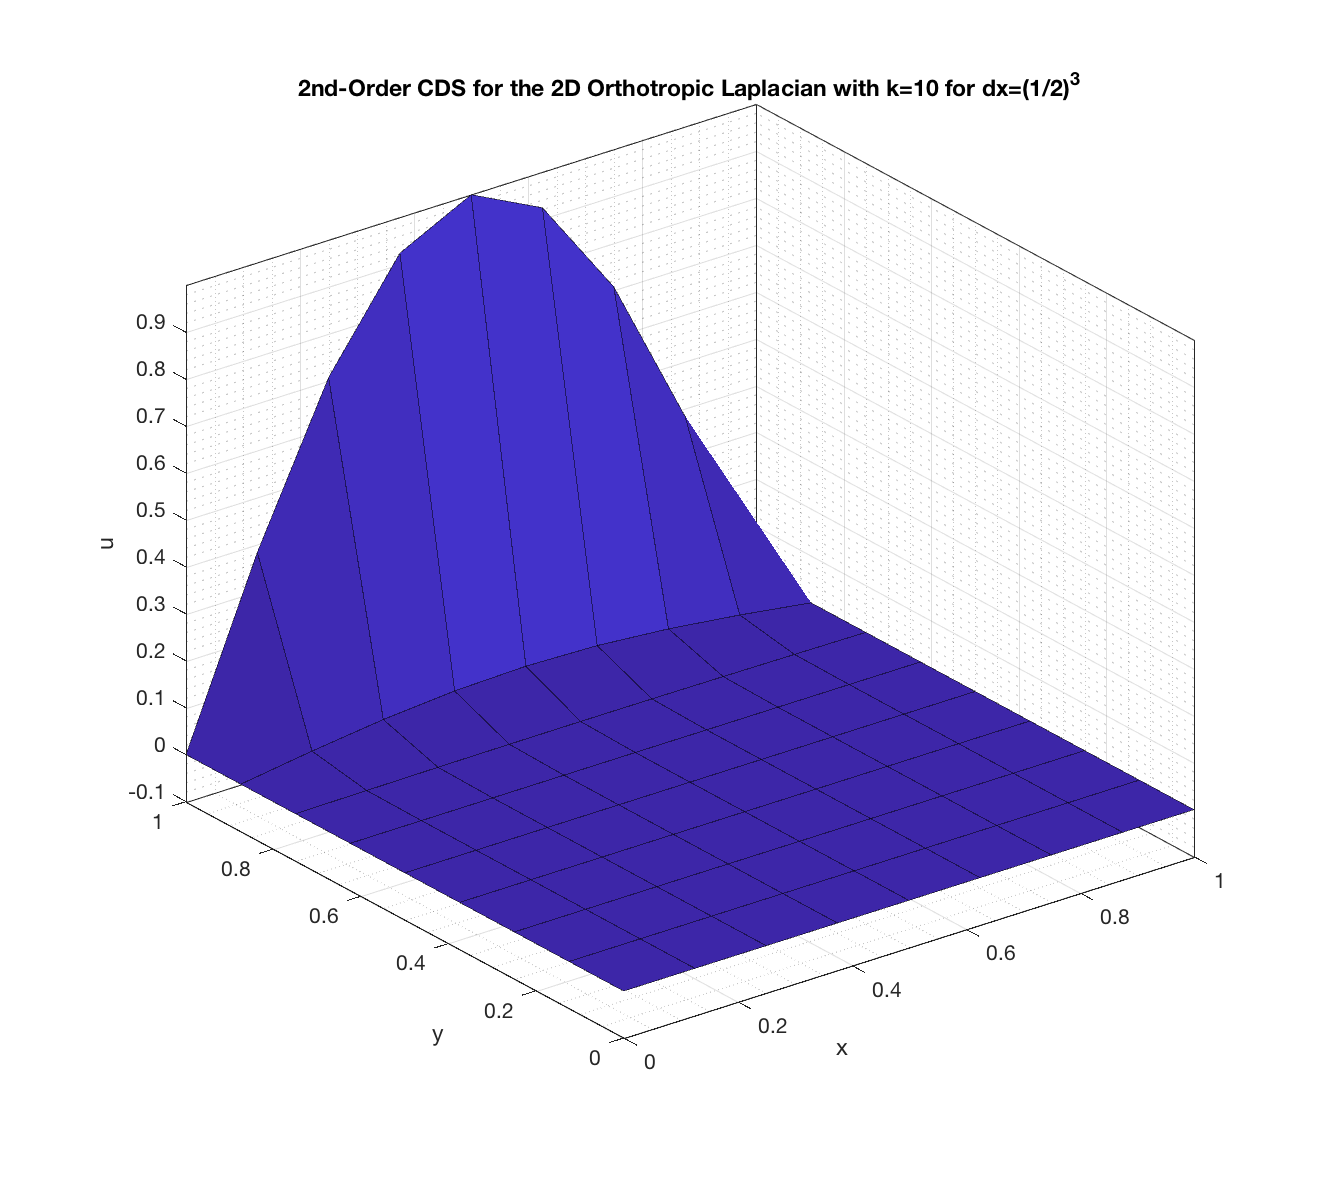
\includegraphics[width = 0.36\linewidth]{surface_order_2_k_10_dx_order_3}
		\includegraphics[width = 0.36\linewidth]{contour_order_2_k_10_dx_order_3}
		\caption{2nd-Order CDS for the 2D Orthotropic Laplacian with $k = 10$ for $\Delta x = (1/2)^3$}
	\end{center}
\end{figure}

\begin{figure}[H]
	\begin{center}
		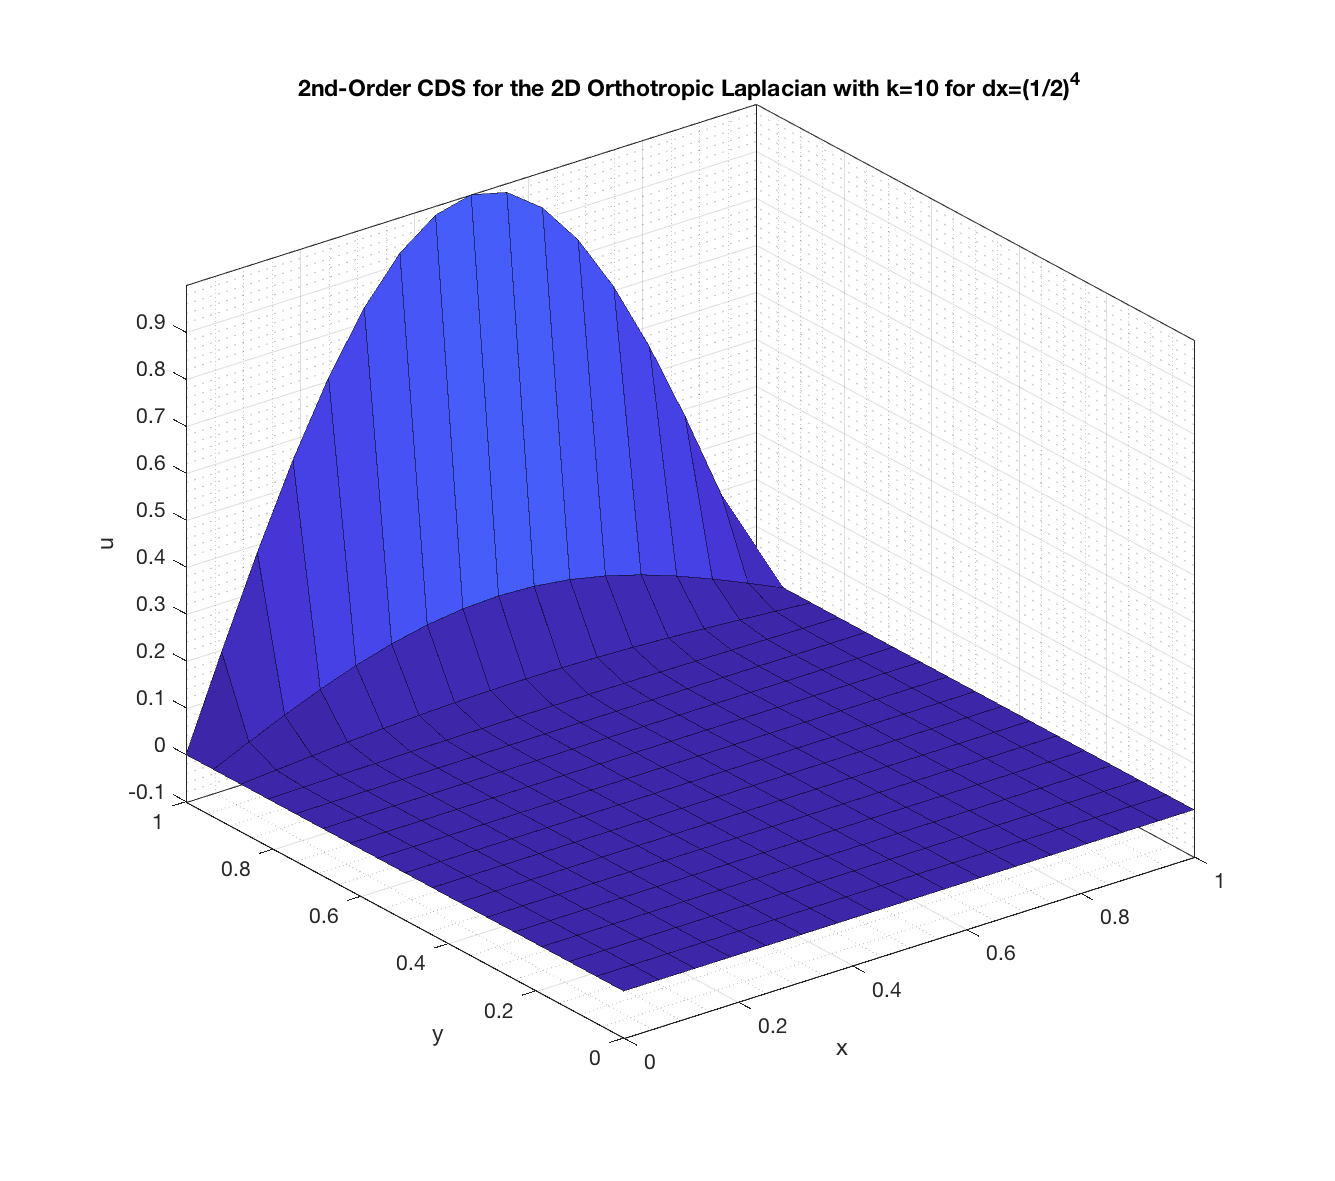
\includegraphics[width = 0.36\linewidth]{surface_order_2_k_10_dx_order_4}
		\includegraphics[width = 0.36\linewidth]{contour_order_2_k_10_dx_order_4}
		\caption{2nd-Order CDS for the 2D Orthotropic Laplacian with $k = 10$ for $\Delta x = (1/2)^4$}
	\end{center}
\end{figure}

\begin{figure}[H]
	\begin{center}
		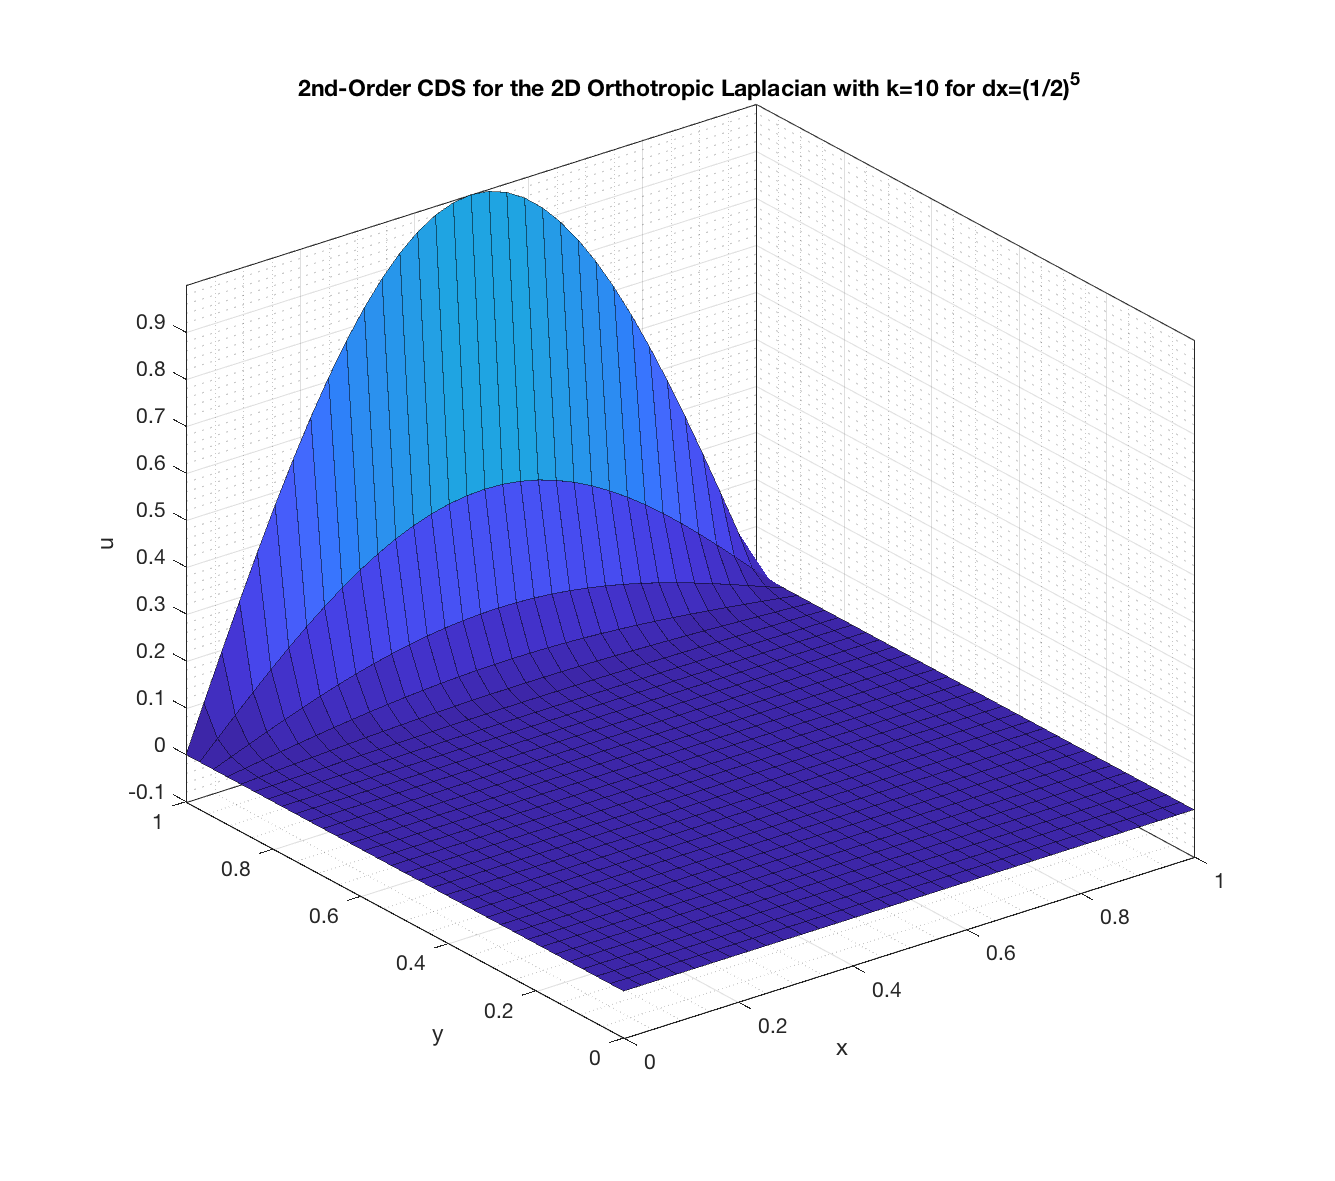
\includegraphics[width = 0.36\linewidth]{surface_order_2_k_10_dx_order_5}
		\includegraphics[width = 0.36\linewidth]{contour_order_2_k_10_dx_order_5}
		\caption{2nd-Order CDS for the 2D Orthotropic Laplacian with $k = 10$ for $\Delta x = (1/2)^5$}
	\end{center}
\end{figure}

\begin{figure}[H]
	\begin{center}
		\includegraphics[width = 0.36\linewidth]{surface_order_2_k_10_dx_order_6}
		\includegraphics[width = 0.36\linewidth]{contour_order_2_k_10_dx_order_6}
		\caption{2nd-Order CDS for the 2D Orthotropic Laplacian with $k = 10$ for $\Delta x = (1/2)^6$}
	\end{center}
\end{figure}

\newpage

\begin{figure}[H]
	\begin{center}
		\includegraphics[width = 0.36\linewidth]{surface_order_2_k_20_dx_order_1}
		\includegraphics[width = 0.36\linewidth]{contour_order_2_k_20_dx_order_1}
		\caption{2nd-Order CDS for the 2D Orthotropic Laplacian with $k = 20$ for $\Delta x = (1/2)^1$}
	\end{center}
\end{figure}

\begin{figure}[H]
	\begin{center}
		\includegraphics[width = 0.36\linewidth]{surface_order_2_k_20_dx_order_2}
		\includegraphics[width = 0.36\linewidth]{contour_order_2_k_20_dx_order_2}
		\caption{2nd-Order CDS for the 2D Orthotropic Laplacian with $k = 20$ for $\Delta x = (1/2)^2$}
	\end{center}
\end{figure}

\begin{figure}[H]
	\begin{center}
		\includegraphics[width = 0.36\linewidth]{surface_order_2_k_20_dx_order_3}
		\includegraphics[width = 0.36\linewidth]{contour_order_2_k_20_dx_order_3}
		\caption{2nd-Order CDS for the 2D Orthotropic Laplacian with $k = 20$ for $\Delta x = (1/2)^3$}
	\end{center}
\end{figure}

\begin{figure}[H]
	\begin{center}
		\includegraphics[width = 0.36\linewidth]{surface_order_2_k_20_dx_order_4}
		\includegraphics[width = 0.36\linewidth]{contour_order_2_k_20_dx_order_4}
		\caption{2nd-Order CDS for the 2D Orthotropic Laplacian with $k = 20$ for $\Delta x = (1/2)^4$}
	\end{center}
\end{figure}

\begin{figure}[H]
	\begin{center}
		\includegraphics[width = 0.36\linewidth]{surface_order_2_k_20_dx_order_5}
		\includegraphics[width = 0.36\linewidth]{contour_order_2_k_20_dx_order_5}
		\caption{2nd-Order CDS for the 2D Orthotropic Laplacian with $k = 20$ for $\Delta x = (1/2)^5$}
	\end{center}
\end{figure}

\begin{figure}[H]
	\begin{center}
		\includegraphics[width = 0.36\linewidth]{surface_order_2_k_20_dx_order_6}
		\includegraphics[width = 0.36\linewidth]{contour_order_2_k_20_dx_order_6}
		\caption{2nd-Order CDS for the 2D Orthotropic Laplacian with $k = 20$ for $\Delta x = (1/2)^6$}
	\end{center}
\end{figure}

\newpage

\begin{figure}[H]
	\begin{center}
		\includegraphics[width = 0.36\linewidth]{surface_order_2_k_50_dx_order_1}
		\includegraphics[width = 0.36\linewidth]{contour_order_2_k_50_dx_order_1}
		\caption{2nd-Order CDS for the 2D Orthotropic Laplacian with $k = 50$ for $\Delta x = (1/2)^1$}
	\end{center}
\end{figure}

\begin{figure}[H]
	\begin{center}
		\includegraphics[width = 0.36\linewidth]{surface_order_2_k_50_dx_order_2}
		\includegraphics[width = 0.36\linewidth]{contour_order_2_k_50_dx_order_2}
		\caption{2nd-Order CDS for the 2D Orthotropic Laplacian with $k = 50$ for $\Delta x = (1/2)^2$}
	\end{center}
\end{figure}

\begin{figure}[H]
	\begin{center}
		\includegraphics[width = 0.36\linewidth]{surface_order_2_k_50_dx_order_3}
		\includegraphics[width = 0.36\linewidth]{contour_order_2_k_50_dx_order_3}
		\caption{2nd-Order CDS for the 2D Orthotropic Laplacian with $k = 50$ for $\Delta x = (1/2)^3$}
	\end{center}
\end{figure}

\begin{figure}[H]
	\begin{center}
		\includegraphics[width = 0.36\linewidth]{surface_order_2_k_50_dx_order_4}
		\includegraphics[width = 0.36\linewidth]{contour_order_2_k_50_dx_order_4}
		\caption{2nd-Order CDS for the 2D Orthotropic Laplacian with $k = 50$ for $\Delta x = (1/2)^4$}
	\end{center}
\end{figure}

\begin{figure}[H]
	\begin{center}
		\includegraphics[width = 0.36\linewidth]{surface_order_2_k_50_dx_order_5}
		\includegraphics[width = 0.36\linewidth]{contour_order_2_k_50_dx_order_5}
		\caption{2nd-Order CDS for the 2D Orthotropic Laplacian with $k = 50$ for $\Delta x = (1/2)^5$}
	\end{center}
\end{figure}

\begin{figure}[H]
	\begin{center}
		\includegraphics[width = 0.36\linewidth]{surface_order_2_k_50_dx_order_6}
		\includegraphics[width = 0.36\linewidth]{contour_order_2_k_50_dx_order_6}
		\caption{2nd-Order CDS for the 2D Orthotropic Laplacian with $k = 50$ for $\Delta x = (1/2)^6$}
	\end{center}
\end{figure}

\newpage

\subsubsection{4th-Order Central Difference Scheme}

\begin{figure}[H]
	\begin{center}
		\includegraphics[width = 0.36\linewidth]{surface_order_4_k_1_dx_order_1}
		\includegraphics[width = 0.36\linewidth]{contour_order_4_k_1_dx_order_1}
		\caption{4th-Order CDS for the 2D Orthotropic Laplacian with $k = 1$ for $\Delta x = (1/2)^1$}
	\end{center}
\end{figure}

\begin{figure}[H]
	\begin{center}
		\includegraphics[width = 0.36\linewidth]{surface_order_4_k_1_dx_order_2}
		\includegraphics[width = 0.36\linewidth]{contour_order_4_k_1_dx_order_2}
		\caption{4th-Order CDS for the 2D Orthotropic Laplacian with $k = 1$ for $\Delta x = (1/2)^2$}
	\end{center}
\end{figure}

\begin{figure}[H]
	\begin{center}
		\includegraphics[width = 0.36\linewidth]{surface_order_4_k_1_dx_order_3}
		\includegraphics[width = 0.36\linewidth]{contour_order_4_k_1_dx_order_3}
		\caption{4th-Order CDS for the 2D Orthotropic Laplacian with $k = 1$ for $\Delta x = (1/2)^3$}
	\end{center}
\end{figure}

\begin{figure}[H]
	\begin{center}
		\includegraphics[width = 0.36\linewidth]{surface_order_4_k_1_dx_order_4}
		\includegraphics[width = 0.36\linewidth]{contour_order_4_k_1_dx_order_4}
		\caption{4th-Order CDS for the 2D Orthotropic Laplacian with $k = 1$ for $\Delta x = (1/2)^4$}
	\end{center}
\end{figure}

\begin{figure}[H]
	\begin{center}
		\includegraphics[width = 0.36\linewidth]{surface_order_4_k_1_dx_order_5}
		\includegraphics[width = 0.36\linewidth]{contour_order_4_k_1_dx_order_5}
		\caption{4th-Order CDS for the 2D Orthotropic Laplacian with $k = 1$ for $\Delta x = (1/2)^5$}
	\end{center}
\end{figure}

\begin{figure}[H]
	\begin{center}
		\includegraphics[width = 0.36\linewidth]{surface_order_4_k_1_dx_order_6}
		\includegraphics[width = 0.36\linewidth]{contour_order_4_k_1_dx_order_6}
		\caption{4th-Order CDS for the 2D Orthotropic Laplacian with $k = 1$ for $\Delta x = (1/2)^6$}
	\end{center}
\end{figure}

\newpage

\begin{figure}[H]
	\begin{center}
		\includegraphics[width = 0.36\linewidth]{surface_order_4_k_2_dx_order_1}
		\includegraphics[width = 0.36\linewidth]{contour_order_4_k_2_dx_order_1}
		\caption{4th-Order CDS for the 2D Orthotropic Laplacian with $k = 2$ for $\Delta x = (1/2)^1$}
	\end{center}
\end{figure}

\begin{figure}[H]
	\begin{center}
		\includegraphics[width = 0.36\linewidth]{surface_order_4_k_2_dx_order_2}
		\includegraphics[width = 0.36\linewidth]{contour_order_4_k_2_dx_order_2}
		\caption{4th-Order CDS for the 2D Orthotropic Laplacian with $k = 2$ for $\Delta x = (1/2)^2$}
	\end{center}
\end{figure}

\begin{figure}[H]
	\begin{center}
		\includegraphics[width = 0.36\linewidth]{surface_order_4_k_2_dx_order_3}
		\includegraphics[width = 0.36\linewidth]{contour_order_4_k_2_dx_order_3}
		\caption{4th-Order CDS for the 2D Orthotropic Laplacian with $k = 2$ for $\Delta x = (1/2)^3$}
	\end{center}
\end{figure}

\begin{figure}[H]
	\begin{center}
		\includegraphics[width = 0.36\linewidth]{surface_order_4_k_2_dx_order_4}
		\includegraphics[width = 0.36\linewidth]{contour_order_4_k_2_dx_order_4}
		\caption{4th-Order CDS for the 2D Orthotropic Laplacian with $k = 2$ for $\Delta x = (1/2)^4$}
	\end{center}
\end{figure}

\begin{figure}[H]
	\begin{center}
		\includegraphics[width = 0.36\linewidth]{surface_order_4_k_2_dx_order_5}
		\includegraphics[width = 0.36\linewidth]{contour_order_4_k_2_dx_order_5}
		\caption{4th-Order CDS for the 2D Orthotropic Laplacian with $k = 2$ for $\Delta x = (1/2)^5$}
	\end{center}
\end{figure}

\begin{figure}[H]
	\begin{center}
		\includegraphics[width = 0.36\linewidth]{surface_order_4_k_2_dx_order_6}
		\includegraphics[width = 0.36\linewidth]{contour_order_4_k_2_dx_order_6}
		\caption{4th-Order CDS for the 2D Orthotropic Laplacian with $k = 2$ for $\Delta x = (1/2)^6$}
	\end{center}
\end{figure}

\newpage

\begin{figure}[H]
	\begin{center}
		\includegraphics[width = 0.36\linewidth]{surface_order_4_k_5_dx_order_1}
		\includegraphics[width = 0.36\linewidth]{contour_order_4_k_5_dx_order_1}
		\caption{4th-Order CDS for the 2D Orthotropic Laplacian with $k = 5$ for $\Delta x = (1/2)^1$}
	\end{center}
\end{figure}

\begin{figure}[H]
	\begin{center}
		\includegraphics[width = 0.36\linewidth]{surface_order_4_k_5_dx_order_2}
		\includegraphics[width = 0.36\linewidth]{contour_order_4_k_5_dx_order_2}
		\caption{4th-Order CDS for the 2D Orthotropic Laplacian with $k = 5$ for $\Delta x = (1/2)^2$}
	\end{center}
\end{figure}

\begin{figure}[H]
	\begin{center}
		\includegraphics[width = 0.36\linewidth]{surface_order_4_k_5_dx_order_3}
		\includegraphics[width = 0.36\linewidth]{contour_order_4_k_5_dx_order_3}
		\caption{4th-Order CDS for the 2D Orthotropic Laplacian with $k = 5$ for $\Delta x = (1/2)^3$}
	\end{center}
\end{figure}

\begin{figure}[H]
	\begin{center}
		\includegraphics[width = 0.36\linewidth]{surface_order_4_k_5_dx_order_4}
		\includegraphics[width = 0.36\linewidth]{contour_order_4_k_5_dx_order_4}
		\caption{4th-Order CDS for the 2D Orthotropic Laplacian with $k = 5$ for $\Delta x = (1/2)^4$}
	\end{center}
\end{figure}

\begin{figure}[H]
	\begin{center}
		\includegraphics[width = 0.36\linewidth]{surface_order_4_k_5_dx_order_5}
		\includegraphics[width = 0.36\linewidth]{contour_order_4_k_5_dx_order_5}
		\caption{4th-Order CDS for the 2D Orthotropic Laplacian with $k = 5$ for $\Delta x = (1/2)^5$}
	\end{center}
\end{figure}

\begin{figure}[H]
	\begin{center}
		\includegraphics[width = 0.36\linewidth]{surface_order_4_k_5_dx_order_6}
		\includegraphics[width = 0.36\linewidth]{contour_order_4_k_5_dx_order_6}
		\caption{4th-Order CDS for the 2D Orthotropic Laplacian with $k = 5$ for $\Delta x = (1/2)^6$}
	\end{center}
\end{figure}

\newpage

\begin{figure}[H]
	\begin{center}
		\includegraphics[width = 0.36\linewidth]{surface_order_4_k_10_dx_order_1}
		\includegraphics[width = 0.36\linewidth]{contour_order_4_k_10_dx_order_1}
		\caption{4th-Order CDS for the 2D Orthotropic Laplacian with $k = 10$ for $\Delta x = (1/2)^1$}
	\end{center}
\end{figure}

\begin{figure}[H]
	\begin{center}
		\includegraphics[width = 0.36\linewidth]{surface_order_4_k_10_dx_order_2}
		\includegraphics[width = 0.36\linewidth]{contour_order_4_k_10_dx_order_2}
		\caption{4th-Order CDS for the 2D Orthotropic Laplacian with $k = 10$ for $\Delta x = (1/2)^2$}
	\end{center}
\end{figure}

\begin{figure}[H]
	\begin{center}
		\includegraphics[width = 0.36\linewidth]{surface_order_4_k_10_dx_order_3}
		\includegraphics[width = 0.36\linewidth]{contour_order_4_k_10_dx_order_3}
		\caption{4th-Order CDS for the 2D Orthotropic Laplacian with $k = 10$ for $\Delta x = (1/2)^3$}
	\end{center}
\end{figure}

\begin{figure}[H]
	\begin{center}
		\includegraphics[width = 0.36\linewidth]{surface_order_4_k_10_dx_order_4}
		\includegraphics[width = 0.36\linewidth]{contour_order_4_k_10_dx_order_4}
		\caption{4th-Order CDS for the 2D Orthotropic Laplacian with $k = 10$ for $\Delta x = (1/2)^4$}
	\end{center}
\end{figure}

\begin{figure}[H]
	\begin{center}
		\includegraphics[width = 0.36\linewidth]{surface_order_4_k_10_dx_order_5}
		\includegraphics[width = 0.36\linewidth]{contour_order_4_k_10_dx_order_5}
		\caption{4th-Order CDS for the 2D Orthotropic Laplacian with $k = 10$ for $\Delta x = (1/2)^5$}
	\end{center}
\end{figure}

\begin{figure}[H]
	\begin{center}
		\includegraphics[width = 0.36\linewidth]{surface_order_4_k_10_dx_order_6}
		\includegraphics[width = 0.36\linewidth]{contour_order_4_k_10_dx_order_6}
		\caption{4th-Order CDS for the 2D Orthotropic Laplacian with $k = 10$ for $\Delta x = (1/2)^6$}
	\end{center}
\end{figure}

\newpage

\begin{figure}[H]
	\begin{center}
		\includegraphics[width = 0.36\linewidth]{surface_order_4_k_20_dx_order_1}
		\includegraphics[width = 0.36\linewidth]{contour_order_4_k_20_dx_order_1}
		\caption{4th-Order CDS for the 2D Orthotropic Laplacian with $k = 20$ for $\Delta x = (1/2)^1$}
	\end{center}
\end{figure}

\begin{figure}[H]
	\begin{center}
		\includegraphics[width = 0.36\linewidth]{surface_order_4_k_20_dx_order_2}
		\includegraphics[width = 0.36\linewidth]{contour_order_4_k_20_dx_order_2}
		\caption{4th-Order CDS for the 2D Orthotropic Laplacian with $k = 20$ for $\Delta x = (1/2)^2$}
	\end{center}
\end{figure}

\begin{figure}[H]
	\begin{center}
		\includegraphics[width = 0.36\linewidth]{surface_order_4_k_20_dx_order_3}
		\includegraphics[width = 0.36\linewidth]{contour_order_4_k_20_dx_order_3}
		\caption{4th-Order CDS for the 2D Orthotropic Laplacian with $k = 20$ for $\Delta x = (1/2)^3$}
	\end{center}
\end{figure}

\begin{figure}[H]
	\begin{center}
		\includegraphics[width = 0.36\linewidth]{surface_order_4_k_20_dx_order_4}
		\includegraphics[width = 0.36\linewidth]{contour_order_4_k_20_dx_order_4}
		\caption{4th-Order CDS for the 2D Orthotropic Laplacian with $k = 20$ for $\Delta x = (1/2)^4$}
	\end{center}
\end{figure}

\begin{figure}[H]
	\begin{center}
		\includegraphics[width = 0.36\linewidth]{surface_order_4_k_20_dx_order_5}
		\includegraphics[width = 0.36\linewidth]{contour_order_4_k_20_dx_order_5}
		\caption{4th-Order CDS for the 2D Orthotropic Laplacian with $k = 20$ for $\Delta x = (1/2)^5$}
	\end{center}
\end{figure}

\begin{figure}[H]
	\begin{center}
		\includegraphics[width = 0.36\linewidth]{surface_order_4_k_20_dx_order_6}
		\includegraphics[width = 0.36\linewidth]{contour_order_4_k_20_dx_order_6}
		\caption{4th-Order CDS for the 2D Orthotropic Laplacian with $k = 20$ for $\Delta x = (1/2)^6$}
	\end{center}
\end{figure}

\newpage

\begin{figure}[H]
	\begin{center}
		\includegraphics[width = 0.36\linewidth]{surface_order_4_k_50_dx_order_1}
		\includegraphics[width = 0.36\linewidth]{contour_order_4_k_50_dx_order_1}
		\caption{4th-Order CDS for the 2D Orthotropic Laplacian with $k = 50$ for $\Delta x = (1/2)^1$}
	\end{center}
\end{figure}

\begin{figure}[H]
	\begin{center}
		\includegraphics[width = 0.36\linewidth]{surface_order_4_k_50_dx_order_2}
		\includegraphics[width = 0.36\linewidth]{contour_order_4_k_50_dx_order_2}
		\caption{4th-Order CDS for the 2D Orthotropic Laplacian with $k = 50$ for $\Delta x = (1/2)^2$}
	\end{center}
\end{figure}

\begin{figure}[H]
	\begin{center}
		\includegraphics[width = 0.36\linewidth]{surface_order_4_k_50_dx_order_3}
		\includegraphics[width = 0.36\linewidth]{contour_order_4_k_50_dx_order_3}
		\caption{4th-Order CDS for the 2D Orthotropic Laplacian with $k = 50$ for $\Delta x = (1/2)^3$}
	\end{center}
\end{figure}

\begin{figure}[H]
	\begin{center}
		\includegraphics[width = 0.36\linewidth]{surface_order_4_k_50_dx_order_4}
		\includegraphics[width = 0.36\linewidth]{contour_order_4_k_50_dx_order_4}
		\caption{4th-Order CDS for the 2D Orthotropic Laplacian with $k = 50$ for $\Delta x = (1/2)^4$}
	\end{center}
\end{figure}

\begin{figure}[H]
	\begin{center}
		\includegraphics[width = 0.36\linewidth]{surface_order_4_k_50_dx_order_5}
		\includegraphics[width = 0.36\linewidth]{contour_order_4_k_50_dx_order_5}
		\caption{4th-Order CDS for the 2D Orthotropic Laplacian with $k = 50$ for $\Delta x = (1/2)^5$}
	\end{center}
\end{figure}

\begin{figure}[H]
	\begin{center}
		\includegraphics[width = 0.36\linewidth]{surface_order_4_k_50_dx_order_6}
		\includegraphics[width = 0.36\linewidth]{contour_order_4_k_50_dx_order_6}
		\caption{4th-Order CDS for the 2D Orthotropic Laplacian with $k = 50$ for $\Delta x = (1/2)^6$}
	\end{center}
\end{figure}

\newpage

\subsection{Finite Difference Method -- Quantity of Interest Results}

\subsubsection{2nd-Order Central Difference Scheme}

\begin{table}[H]
	\flushleft
	\caption{Quantity of Interest for 2nd-Order CDS FDM for Orthotropic Laplacian}		\begin{tabular}{|c|c|c|c|c|c|c|}
\hline
\textbf{$\Delta x$}&\textbf{$u'_{k^2=1}(1)$}&\textbf{$u'_{k^2=2}(1)$}&\textbf{$\bar{u}'_{k^2=1}(1)$}&\textbf{$\bar{u}'_{k^2=2}(1)$}&\textbf{$\epsilon'_{rel,k^2=1}$}&\textbf{$\epsilon'_{rel,k^2=2}$}\\\hline
0.5000&3.5000&9.8000&3.1533&6.2832&10.9931&55.9708\\\hline
0.2500&3.2946&7.7107&3.1533&6.2832&4.4782&22.7185\\\hline
0.1250&3.1932&6.7013&3.1533&6.2832&1.2630&6.6544\\\hline
0.0625&3.1636&6.3925&3.1533&6.2832&0.3255&1.7398\\\hline
0.0312&3.1559&6.3109&3.1533&6.2832&0.0820&0.4400\\\hline
0.0156&3.1540&6.2902&3.1533&6.2832&0.0205&0.1103\\\hline
0.0078&3.1535&6.2850&3.1533&6.2832&0.0051&0.0276\\\hline
0.0039&3.1534&6.2837&3.1533&6.2832&0.0013&0.0069\\\hline
\end{tabular}

	\begin{tabular}{|c|c|c|c|c|c|c|}
\hline
\textbf{$\Delta x$}&\textbf{$u'_{k^2=5}(1)$}&\textbf{$u'_{k^2=10}(1)$}&\textbf{$\bar{u}'_{k^2=5}(1)$}&\textbf{$\bar{u}'_{k^2=10}(1)$}&\textbf{$\epsilon'_{rel,k^2=5}$}&\textbf{$\epsilon'_{rel,k^2=10}$}\\\hline
0.5000&51.9615&201.9901&15.7080&31.4159&230.7974&542.9545\\\hline
0.2500&33.0481&121.0912&15.7080&31.4159&110.3909&285.4454\\\hline
0.1250&21.8027&68.4303&15.7080&31.4159&38.8004&117.8205\\\hline
0.0625&17.4649&43.9199&15.7080&31.4159&11.1847&39.8015\\\hline
0.0312&16.1673&34.9800&15.7080&31.4159&2.9242&11.3448\\\hline
0.0156&15.8242&32.3449&15.7080&31.4159&0.7399&2.9570\\\hline
0.0078&15.7371&31.6508&15.7080&31.4159&0.1855&0.7476\\\hline
0.0039&15.7153&31.4748&15.7080&31.4159&0.0464&0.1874\\\hline
\end{tabular}

	\begin{tabular}{|c|c|c|c|c|c|c|}
\hline
\textbf{$\Delta x$}&\textbf{$u'_{k^2=1}(1)$}&\textbf{$u'_{k^2=2}(1)$}&\textbf{$\bar{u}'_{k^2=1}(1)$}&\textbf{$\bar{u}'_{k^2=2}(1)$}&\textbf{$\epsilon'_{rel,k^2=1}$}&\textbf{$\epsilon'_{rel,k^2=2}$}\\\hline
0.5000&801.9975&5001.9996&62.8319&157.0796&1176.4187&3084.3718\\\hline
0.2500&472.6122&2932.9295&62.8319&157.0796&652.1857&1767.1609\\\hline
0.1250&251.4583&1530.3884&62.8319&157.0796&300.2083&874.2755\\\hline
0.0625&138.0501&784.4256&62.8319&157.0796&119.7136&399.3809\\\hline
0.0312&87.9978&415.9929&62.8319&157.0796&40.0528&164.8293\\\hline
0.0156&69.9852&248.6217&62.8319&157.0796&11.3849&58.2775\\\hline
0.0078&64.6949&184.2864&62.8319&157.0796&2.9652&17.3204\\\hline
0.0039&63.3028&164.3048&62.8319&157.0796&0.7495&4.5997\\\hline
\end{tabular}

\end{table}

\newpage

\subsubsection{4th-Order Central Difference Scheme}

\begin{table}[H]
	\flushleft
	\caption{Quantity of Interest for 4th-Order CDS FDM for Orthotropic Laplacian}	
	\begin{tabular}{|c|c|c|c|c|c|c|}
\hline
\textbf{$\Delta x$}&\textbf{$u'_{k^2=1}(1)$}&\textbf{$u'_{k^2=2}(1)$}&\textbf{$\bar{u}'_{k^2=1}(1)$}&\textbf{$\bar{u}'_{k^2=2}(1)$}&\textbf{$\epsilon'_{rel,k^2=1}$}&\textbf{$\epsilon'_{rel,k^2=2}$}\\\hline
0.5000&3.4311&8.5487&3.1533&6.2832&8.8067&36.0563\\\hline
0.2500&3.1762&6.5676&3.1533&6.2832&0.7252&4.5264\\\hline
0.1250&3.1549&6.3086&3.1533&6.2832&0.0501&0.4034\\\hline
0.0625&3.1535&6.2851&3.1533&6.2832&0.0032&0.0292\\\hline
0.0312&3.1534&6.2834&3.1533&6.2832&0.0002&0.0019\\\hline
0.0156&3.1533&6.2832&3.1533&6.2832&0.0000&0.0001\\\hline
0.0078&3.1533&6.2832&3.1533&6.2832&0.0000&0.0000\\\hline
0.0039&3.1533&6.2832&3.1533&6.2832&0.0000&0.0000\\\hline
\end{tabular}

	\begin{tabular}{|c|c|c|c|c|c|c|}
\hline
\textbf{$\Delta x$}&\textbf{$u'_{k^2=5}(1)$}&\textbf{$u'_{k^2=10}(1)$}&\textbf{$\bar{u}'_{k^2=5}(1)$}&\textbf{$\bar{u}'_{k^2=10}(1)$}&\textbf{$\epsilon'_{rel,k^2=5}$}&\textbf{$\epsilon'_{rel,k^2=10}$}\\\hline
0.5000&40.8135&155.0190&15.7080&31.4159&159.8266&393.4407\\\hline
0.2500&21.6680&70.7840&15.7080&31.4159&37.9427&125.3124\\\hline
0.1250&16.7136&42.1531&15.7080&31.4159&6.4022&34.1776\\\hline
0.0625&15.8142&33.3020&15.7080&31.4159&0.6766&6.0036\\\hline
0.0312&15.7163&31.6180&15.7080&31.4159&0.0531&0.6431\\\hline
0.0156&15.7085&31.4319&15.7080&31.4159&0.0037&0.0508\\\hline
0.0078&15.7080&31.4170&15.7080&31.4159&0.0002&0.0035\\\hline
0.0039&15.7080&31.4160&15.7080&31.4159&0.0000&0.0002\\\hline
\end{tabular}

	\begin{tabular}{|c|c|c|c|c|c|c|}
\hline
\textbf{$\Delta x$}&\textbf{$u'_{k^2=1}(1)$}&\textbf{$u'_{k^2=2}(1)$}&\textbf{$\bar{u}'_{k^2=1}(1)$}&\textbf{$\bar{u}'_{k^2=2}(1)$}&\textbf{$\epsilon'_{rel,k^2=1}$}&\textbf{$\epsilon'_{rel,k^2=2}$}\\\hline
0.5000&611.6382&3807.8780&62.8319&157.0796&873.4525&2324.1704\\\hline
0.2500&265.7677&1629.8802&62.8319&157.0796&322.9824&937.6140\\\hline
0.1250&136.6632&792.9967&62.8319&157.0796&117.5062&404.8374\\\hline
0.0625&83.7237&410.3829&62.8319&157.0796&33.2504&161.2579\\\hline
0.0312&66.5413&238.0208&62.8319&157.0796&5.9038&51.5287\\\hline
0.0156&63.2307&174.1551&62.8319&157.0796&0.6348&10.8706\\\hline
0.0078&62.8634&159.2087&62.8319&157.0796&0.0502&1.3554\\\hline
0.0039&62.8340&157.2612&62.8319&157.0796&0.0035&0.1156\\\hline
\end{tabular}

\end{table}

\newpage

\section{Convergence Analysis}

\subsection{Rate of Convergence Derivation}

Let the error for a particular mesh size $\Delta x$ be $E\left(\Delta x\right)$:
\begin{equation}
E\left(\Delta x\right) = C\left(\Delta x\right)^\beta
\end{equation}
Then for a smaller mesh size $\frac{\Delta x}{2}$ we have:
\begin{equation}
E\left(\frac{\Delta x}{2}\right) = C\left(\frac{\Delta x}{2}\right)^\beta
\end{equation}
Dividing the error at each mesh size and taking the logarithm:
\begin{equation}
\frac{E\left(\Delta x\right)}{E\left(\frac{\Delta x}{2}\right)} = \frac{C\left(\Delta x\right)^\beta}{C\left(\frac{\Delta x}{2}\right)^\beta} = 2^\beta
\end{equation}
\begin{equation}
\log\left[\frac{E\left(\Delta x\right)}{E\left(\frac{\Delta x}{2}\right)}\right] = \log(2^\beta)
\end{equation}
\begin{equation}
\log\left[\frac{E\left(\Delta x\right)}{E\left(\frac{\Delta x}{2}\right)}\right] = \beta \log(2)
\end{equation}
Rearranging for $\beta$ and simplifying:
\begin{equation}
\beta = \frac{1}{\log(2)} \left[\log\left(E\left(\Delta x\right)\right) - \log\left(E\left(\frac{\Delta x}{2}\right)\right)\right] 
\end{equation}
Denoting $E^*_{\Delta x} = \log\left(E\left(\Delta x\right)\right)$:
\begin{equation}
\mathbf{\beta = \frac{E^*_{\Delta x} - E^*_{\frac{\Delta x}{2}}}{\log (2)}}
\end{equation}

\newpage

\subsection{Rate of Convergence for the Orthotropic Diffusion Equation -- Results}

\subsubsection{2nd-Order Central Difference Scheme}

\begin{figure}[H]
	\begin{center}
		\includegraphics[width = 0.8\linewidth]{order_2_u_y_fdm}
		\caption{Rate of Convergence of QOI for 2nd-Order CDS FDM for Orthotropic Laplacian using FDM for Several Values of $k^2$}	
	\end{center}
\end{figure}

\begin{table}[H]
	\begin{tabular}{|c|c|c|c|c|c|c|}
\hline
\textbf{$\Delta x$}&\textbf{$\beta(k^2=1)$}&\textbf{$\beta(k^2=2)$}&\textbf{$\beta(k^2=5)$}&\textbf{$\beta(k^2=10)$}&\textbf{$\beta(k^2=20)$}&\textbf{$\beta(k^2=50)$}\\\hline
0.5000&1.2956&1.3008&1.0640&0.9276&0.8510&0.8035\\\hline
0.2500&1.8260&1.7715&1.5085&1.2766&1.1193&1.0153\\\hline
0.1250&1.9562&1.9354&1.7945&1.5657&1.3264&1.1303\\\hline
0.0625&1.9890&1.9832&1.9354&1.8108&1.5796&1.2768\\\hline
0.0312&1.9973&1.9958&1.9826&1.9398&1.8148&1.5000\\\hline
0.0156&1.9993&1.9989&1.9956&1.9838&1.9409&1.7505\\\hline
0.0078&1.9998&1.9997&1.9989&1.9959&1.9841&1.9129\\\hline
\end{tabular}

\end{table}

\begin{figure}[H]
	\begin{center}
		\includegraphics[width = 0.8\linewidth]{order_2_u_y_lag}
		\caption{Rate of Convergence of QOI for 2nd-Order CDS FDM for Orthotropic Laplacian using Lagrangian Interpolation for Several Values of $k^2$}	
	\end{center}
\end{figure}

\begin{table}[H]
	\begin{tabular}{|c|c|c|c|c|c|c|}
\hline
\textbf{$\Delta x$}&\textbf{$\beta(k^2=1)$}&\textbf{$\beta(k^2=2)$}&\textbf{$\beta(k^2=5)$}&\textbf{$\beta(k^2=10)$}&\textbf{$\beta(k^2=20)$}&\textbf{$\beta(k^2=50)$}\\\hline
0.5000&1.2629&0.7997&0.3283&0.1545&0.0735&0.0283\\\hline
0.2500&1.6151&1.2646&0.6645&0.3293&0.1546&0.0581\\\hline
0.1250&1.8140&1.6151&1.1275&0.6662&0.3295&0.1214\\\hline
0.0625&1.9104&1.8092&1.5231&1.1288&0.6666&0.2586\\\hline
0.0312&1.9563&1.9060&1.7592&1.5234&1.1291&0.5385\\\hline
0.0156&1.9784&1.9535&1.8805&1.7590&1.5234&0.9778\\\hline
0.0078&1.9893&1.9769&1.9407&1.8803&1.7590&1.4137\\\hline
\end{tabular}

\end{table}

\begin{figure}[H]
	\begin{center}
		\includegraphics[width = 0.8\linewidth]{order_2_u_avg}
		\caption{Rate of Convergence of $u(1/2, 1/2)$ for 2nd-Order CDS FDM for Orthotropic Laplacian for Several Values of $k^2$}	
	\end{center}
\end{figure}

\begin{table}[H]
	\begin{tabular}{|c|c|c|c|c|c|c|}
\hline
\textbf{$\Delta x$}&\textbf{$\beta(k^2=1)$}&\textbf{$\beta(k^2=2)$}&\textbf{$\beta(k^2=5)$}&\textbf{$\beta(k^2=10)$}&\textbf{$\beta(k^2=20)$}&\textbf{$\beta(k^2=50)$}\\\hline
0.5000&1.8452&1.8144&2.5366&4.1832&6.1216&8.7480\\\hline
0.2500&1.9530&1.9275&2.4165&4.5834&8.1291&13.2825\\\hline
0.1250&1.9875&1.9784&2.1813&3.8466&9.0131&18.6064\\\hline
0.0625&1.9968&1.9943&2.0552&2.7491&7.2055&22.3156\\\hline
0.0312&1.9992&1.9986&2.0146&2.2166&4.1086&20.1556\\\hline
0.0156&1.9998&1.9996&2.0037&2.0561&2.5699&11.8100\\\hline
0.0078&2.0000&1.9999&2.0009&2.0142&2.1423&4.9235\\\hline
\end{tabular}

\end{table}

\newpage

\subsubsection{4th-Order Central Difference Scheme}

\begin{figure}[H]
	\begin{center}
		\includegraphics[width = 0.8\linewidth]{order_4_u_y_fdm}
		\caption{Rate of Convergence of QOI for 4th-Order CDS FDM for Orthotropic Laplacian using FDM for Several Values of $k^2$}	
	\end{center}
\end{figure}

\begin{table}[H]
	\begin{tabular}{|c|c|c|c|c|c|c|}
\hline
\textbf{$\Delta x$}&\textbf{$\beta(k^2=1)$}&\textbf{$\beta(k^2=2)$}&\textbf{$\beta(k^2=5)$}&\textbf{$\beta(k^2=10)$}&\textbf{$\beta(k^2=20)$}&\textbf{$\beta(k^2=50)$}\\\hline
0.5000&3.6021&2.9938&2.0746&1.6506&1.4353&1.3096\\\hline
0.2500&3.8543&3.4881&2.5672&1.8744&1.4587&1.2117\\\hline
0.1250&3.9522&3.7879&3.2423&2.5092&1.8213&1.3280\\\hline
0.0625&3.9834&3.9115&3.6713&3.2226&2.4937&1.6459\\\hline
0.0312&3.9936&3.9606&3.8595&3.6625&3.2174&2.2449\\\hline
0.0156&3.9973&3.9816&3.9368&3.8551&3.6602&3.0036\\\hline
0.0078&4.0002&3.9910&3.9702&3.9345&3.8540&3.5513\\\hline
\end{tabular}

\end{table}

\begin{figure}[H]
	\begin{center}
		\includegraphics[width = 0.8\linewidth]{order_4_u_y_lag}
		\caption{Rate of Convergence of QOI for 4th-Order CDS FDM for Orthotropic Laplacian using Lagrangian Interpolation for Several Values of $k^2$}	
	\end{center}
\end{figure}

\begin{table}[H]
	\begin{tabular}{|c|c|c|c|c|c|c|}
\hline
\textbf{$\Delta x$}&\textbf{$\beta(k^2=1)$}&\textbf{$\beta(k^2=2)$}&\textbf{$\beta(k^2=5)$}&\textbf{$\beta(k^2=10)$}&\textbf{$\beta(k^2=20)$}&\textbf{$\beta(k^2=50)$}\\\hline
0.5000&3.7057&2.1425&0.8117&0.3658&0.1691&0.0639\\\hline
0.2500&3.1863&2.4663&1.2924&0.6233&0.2807&0.1011\\\hline
0.1250&3.5589&3.1411&2.1875&1.2923&0.6233&0.2177\\\hline
0.0625&3.7720&3.5472&2.9537&2.1874&1.2923&0.4827\\\hline
0.0312&3.8842&3.7677&3.4407&2.9537&2.1874&1.0389\\\hline
0.0156&3.9416&3.8823&3.7112&3.4407&2.9537&1.8967\\\hline
0.0078&3.9705&3.9408&3.8533&3.7112&3.4407&2.7368\\\hline
\end{tabular}

\end{table}

\begin{figure}[H]
	\begin{center}
		\includegraphics[width = 0.8\linewidth]{order_4_u_avg}
		\caption{Rate of Convergence of $u(1/2, 1/2)$ for 4th-Order CDS FDM for Orthotropic Laplacian for Several Values of $k^2$}	
	\end{center}
\end{figure}

\begin{table}[H]
	\begin{tabular}{|c|c|c|c|c|c|c|}
\hline
\textbf{$\Delta x$}&\textbf{$\beta(k^2=1)$}&\textbf{$\beta(k^2=2)$}&\textbf{$\beta(k^2=5)$}&\textbf{$\beta(k^2=10)$}&\textbf{$\beta(k^2=20)$}&\textbf{$\beta(k^2=50)$}\\\hline
0.5000&6.0343&3.9672&11.6693&3.9518&3.4464&3.3169\\\hline
0.2500&6.0026&3.9177&-1.7517&18.6408&7.9315&6.8094\\\hline
0.1250&6.0002&3.9736&3.8180&-1.9066&33.0333&14.8570\\\hline
0.0625&6.0000&3.9930&3.9580&3.6717&-1.7018&42.8940\\\hline
0.0312&5.9795&3.9982&3.9896&3.9482&3.3977&42.1099\\\hline
0.0156&3.7530&3.9995&3.9974&3.9890&3.9284&1.7375\\\hline
0.0078&-1.6341&3.9992&3.9993&3.9974&3.9877&3.7254\\\hline
\end{tabular}

\end{table}

\newpage

\section{Discussion}

There are a few things to note in the discussion of the results:

First, the results of the second-order and fourth-order methods yield, on the whole, second-order and fourth-order convergence on the grid and second-order and fourth-order convergence of the quantity of interest.

Second, the Lagrangian interpolant performs essentially as well as required by the order of convergence of the method.

Finally, there are a few small spurious oscillations that only arise in the fourth-order case. This may be due to roundoff error arising and propagating. However, it appears that this may be a function grid size and diffusivity constant $k^2$. This is reminiscent of the P\'eclet condition that required a certain ratio of the mesh spacing and diffusivity to be satisfied or the oscillations would develop. However, the lack of these oscillations in the second-order case leads to the assumption that it is some kind of minor code error or roundoff error accumulation.

A simultaneous comparison of all of the methods for various values of $k$ proves that:

\begin{itemize}
	\item the second-order central difference scheme finite difference method is quadratically convergent
	\item the fourth-order central difference scheme finite difference method is quartically convergent
\end{itemize}

\newpage

\appendix

\section{$u(x)$ v. $u_{exact}(x)$ Tables}

\textit{Error tables are available for all mesh spacings through the MATLAB code or by request} (ross.alexander19@tamu.edu). The tables are not printed here due to printing constraints.

\newpage

\section{MATLAB Code}

\subsection{homework\_5\_code\_order\_2.m}

\begin{lstlisting}
clear all; close all; clc
%#ok<*SPRIX>
%#ok<*CTCH>
%#ok<*UNRCH>
%#ok<*CLALL>
%#ok<*SAGROW>

%% 2nd-Order

meshOrder   = 1:8;
meshDx      = 1./(2.^meshOrder);

genFigSurface   = false;
genFigContour   = false;
genFigROC       = false;
genFigAvg       = false;
genFigLag       = false;
tableSave       = true;

rowID = 0;
colID = 0;

matNumTotal = length(meshOrder)*6;
matNum = 0;

for k = [1 2 5 10 20 50]

rowID = rowID + 1;
colID = 0;

for order = meshOrder

matNum = matNum + 1;

clc
fprintf('solving matrix %i/%i\n', matNum, matNumTotal)

colID = colID + 1;

clear A ARow b u U

dx = 1/(2^order);
n = 1/dx;

A = assemble(n, k, 2);

b = sparse((n-1)^2, 1);

for i = (n-1)*(n-2)+1:(n-1)^2

xi = (i-(n-1)*(n-2))*dx;
b(i) = sin(pi*xi);

end

u = A\b;

u = reshape(u, n-1, n-1)';
U = zeros(n+1, n+1);
U(2:end-1, 2:end-1) = u;

x = linspace(0, 1, n+1);
y = linspace(0, 1, n+1);

[X, Y] = meshgrid(x, y);

U(end, :) = sin(pi.*x);

titleString = strcat('2nd-Order CDS for the 2D Orthotropic Laplacian with k=', ...
num2str(k), ' for dx=(1/2)^', num2str(order));
figureString = strcat('order_2_k_', num2str(k), '_dx_order_', num2str(order));

if genFigSurface
figSurface(X, Y, U, titleString, figureString);
end

if genFigContour
figContour(X, Y, U, titleString, figureString);
end

[dim, ~] = size(U);
avg = (dim+1)/2;

[~, Lprime] = lagrange(dx, avg, U, 2);

uavgfdm(rowID, colID) = U(avg, avg);
uavgexact(rowID, colID) = sin(pi/2)*sinh(k*pi/2)/sinh(k*pi);
uyfdm(rowID, colID) = 1 / dx * ((1+k^2)*U(end, avg) - U(end-1, avg) - k^2/2*U(end, avg-1) - k^2/2*U(end, avg+1));
uyexact(rowID, colID) = k*pi*coth(k*pi);
uylag(rowID, colID) = double(subs(Lprime, 1));

clear xl

end

end

relError = abs(uyexact-uyfdm) ./ abs(uyexact) * 100;
relErrorAvg = abs(uavgexact-uavgfdm) ./ abs(uavgexact) * 100; %#ok<NASGU>
relErrorLag = abs(uyexact-uylag) ./ abs(uyexact) * 100;
logRelError = log10(relError);
logRelErrorLag = log10(relErrorLag);
logRelErrorAvg = log10(relErrorAvg);

for kID = 1:6

try
for rocID = 1:length(logRelError) - 1
roc(kID, rocID) = (logRelError(kID, rocID+1) - logRelError(kID, rocID)) / -log10(2);
rocLag(kID, rocID) = (logRelErrorLag(kID, rocID+1) - logRelErrorLag(kID, rocID)) / -log10(2);
rocAvg(kID, rocID) = (logRelErrorAvg(kID, rocID+1) - logRelErrorAvg(kID, rocID)) / -log10(2);
end
catch
for rocID = 1:length(logRelError) - 2
roc(kID, rocID) = (logRelError(kID, rocID+1) - logRelError(kID, rocID)) / -log10(2);
rocLag(kID, rocID) = (logRelErrorLag(kID, rocID+1) - logRelErrorLag(kID, rocID)) / -log10(2);
rocAvg(kID, rocID) = (logRelErrorAvg(kID, rocID+1) - logRelErrorAvg(kID, rocID)) / -log10(2);
end
end

end

if genFigAvg
figAvg(2, meshDx, relErrorAvg);
end

if genFigROC
figRoc(2, meshDx, relError);
end

if genFigLag
figLag(2, meshDx, relErrorLag);
end

if tableSave
tableRender(2, meshDx, roc, rocLag, rocAvg, uyfdm, uyexact, relError);
end
\end{lstlisting}

\subsection{homework\_5\_code\_order\_4.m}

\begin{lstlisting}
clear all; close all; clc
%#ok<*SPRIX>
%#ok<*CTCH>
%#ok<*UNRCH>
%#ok<*CLALL>
%#ok<*SAGROW>

%% 4th-Order

meshOrder   = 1:8;
meshDx      = 1./(2.^meshOrder);

genFigSurface   = false;
genFigContour   = false;
genFigROC       = false;
genFigAvg       = false;
genFigLag       = false;
tableSave       = true;

rowID = 0;
colID = 0;

matNumTotal = length(meshOrder)*6;
matNum = 0;

for k = [1 2 5 10 20 50]

rowID = rowID + 1;
colID = 0;

for order = meshOrder

matNum = matNum + 1;

clc
fprintf('solving matrix %i/%i\n', matNum, matNumTotal)

colID = colID + 1;

clear A ARow b u U C d uy

dx = 1/(2^order);
n = 1/dx;

A = assemble(n, k, 4);

b = sparse((n-1)^2, 1);

for i = (n-1)*(n-2)+1:(n-1)^2

xl = (i-1-(n-1)*(n-2))*dx;
xc = (i-(n-1)*(n-2))*dx;
xr = (i+1-(n-1)*(n-2))*dx;
b(i) = -(k^2/12+1/12)*(sin(pi*xl)+sin(pi*xr))-(1-k^2/6-1/6)*sin(pi*xc);

end

u = A\b;

u = reshape(u, n-1, n-1)';
U = zeros(n+1, n+1);
U(2:end-1, 2:end-1) = u;

x = linspace(0, 1, n+1);
y = linspace(0, 1, n+1);

[X, Y] = meshgrid(x, y);

U(end, :) = sin(pi.*x);

titleString = strcat('4th-Order CDS for the 2D Orthotropic Laplacian with k=', ...
num2str(k), ' for dx=(1/2)^', num2str(order));
figureString = strcat('order_4_k_', num2str(k), '_dx_order_', num2str(order));

if genFigSurface
figSurface(X, Y, U, titleString, figureString);
end

if genFigContour
figContour(X, Y, U, titleString, figureString);
end

[dim, ~] = size(U);
avg = (dim+1)/2;

alpha = -k^2/6;
beta = 1 + k^2/3;
C = sparse(gallery('tridiag', n+1, alpha, beta, alpha));
C(1, 1) = 1;
C(1, 2) = 0;
C(end, end-1) = 0;
C(end, end) = 1;

d = sparse(n+1, 1);

for i = 2:n
d(i) = U(end, i)/dx - U(end-1, i)/dx + (k^2*pi^2*dx)/2*U(end, i) + (k^4*pi^4*dx^3)/24*U(end, i);
end

uy = C\d;

[~, Lprime] = lagrange(dx, avg, U, 4);

uavgfdm(rowID, colID) = U(avg, avg);
uavgexact(rowID, colID) = sin(pi/2)*sinh(k*pi/2)/sinh(k*pi);
uyfdm(rowID, colID) = uy(avg);
uyexact(rowID, colID) = k*pi*coth(k*pi);
uylag(rowID, colID) = double(subs(Lprime, 1));

clear xl

end

end

relError = abs(uyexact-uyfdm) ./ abs(uyexact) * 100;
relErrorAvg = abs(uavgexact-uavgfdm) ./ abs(uavgexact) * 100;
relErrorLag = abs(uyexact-uylag) ./ abs(uyexact) * 100;
logRelError = log10(relError);
logRelErrorLag = log10(relErrorLag);
logRelErrorAvg = log10(relErrorAvg);

for kID = 1:6

try
for rocID = 1:length(logRelError) - 1
roc(kID, rocID) = (logRelError(kID, rocID+1) - logRelError(kID, rocID)) / -log10(2);
rocLag(kID, rocID) = (logRelErrorLag(kID, rocID+1) - logRelErrorLag(kID, rocID)) / -log10(2);
rocAvg(kID, rocID) = (logRelErrorAvg(kID, rocID+1) - logRelErrorAvg(kID, rocID)) / -log10(2);
end
catch
for rocID = 1:length(logRelError) - 2
roc(kID, rocID) = (logRelError(kID, rocID+1) - logRelError(kID, rocID)) / -log10(2);
rocLag(kID, rocID) = (logRelErrorLag(kID, rocID+1) - logRelErrorLag(kID, rocID)) / -log10(2);
rocAvg(kID, rocID) = (logRelErrorAvg(kID, rocID+1) - logRelErrorAvg(kID, rocID)) / -log10(2);
end
end

end

if genFigAvg
figAvg(4, meshDx, relErrorAvg);
end

if genFigROC
figAvg(4, meshDx, relError);
end

if genFigLag
figLag(4, meshDx, relErrorLag);
end

if tableSave
tableRender(4, meshDx, roc, rocLag, rocAvg, uyfdm, uyexact, relError);
end
\end{lstlisting}

\subsection{assemble.m}

\begin{lstlisting}
function [ A ] = assemble( n, k, order )

ac = sparse(zeros(n-1, n-1));
ai = sparse(zeros(n-1, n-1));
az = sparse(zeros(n-1, n-1));

if order == 2

for i = 1:(n-1)
for j = 1:(n-1)

if i == j
ac(i, j) = 2+2*k^2;
ai(i, j) = -1;
elseif abs(i - j) == 1
ac(i, j) = -k^2;
ai(i, j) = 0;
end

end
end

elseif order == 4

for i = 1:(n-1)
for j = 1:(n-1)

if i == j
ac(i, j) = (-2+1/3)*(k^2+1);
ai(i, j) = 1-k^2/6-1/6;
elseif abs(i - j) == 1
ac(i, j) = k^2-k^2/6-1/6;
ai(i, j) = k^2/12+1/12;
end

end
end

else
error('Invalid order.')
end

for i = 1:(n-1)

for j = 1:(n-1)

if j == 1 && i == j
ARow = ac;
elseif j == 1 && abs(i - j) == 1
ARow = ai;
elseif j == 1 && abs(i - j) > 1
ARow = az;
elseif i == j
ARow = [ARow ac];
elseif abs(i - j) == 1
ARow = [ARow ai];
elseif abs(i - j) > 1
ARow = [ARow az];
end

end

if i == 1
A = [ARow];
else
A = [A; ARow];
end

end

end
\end{lstlisting}

\subsection{lagrange.m}

\begin{lstlisting}
function [ L, Lprime ] = lagrange( dx, avg, U, lorder )

x0 = 1;
x1 = 1-dx;
x2 = 1-2*dx;
x3 = 1-3*dx;
x4 = 1-4*dx;
x5 = 1-5*dx;

syms xl

if lorder == 2
lp0 = ((xl-x1)*(xl-x2))/((x0-x1)*(x0-x2));
lp1 = ((xl-x0)*(xl-x2))/((x1-x0)*(x1-x2));
lp2 = ((xl-x0)*(xl-x1))/((x2-x0)*(x2-x1));

L = U(end, avg)*lp0 + U(end-1, avg)*lp1 + U(end-2, avg)*lp2;
end

if lorder == 4
try
lp0 = ((xl-x1)*(xl-x2)*(xl-x3)*(xl-x4))/((x0-x1)*(x0-x2)*(x0-x3)*(x0-x4));
lp1 = ((xl-x0)*(xl-x2)*(xl-x3)*(xl-x4))/((x1-x0)*(x1-x2)*(x1-x3)*(x1-x4));
lp2 = ((xl-x0)*(xl-x1)*(xl-x3)*(xl-x4))/((x2-x0)*(x2-x1)*(x2-x3)*(x2-x4));
lp3 = ((xl-x0)*(xl-x1)*(xl-x2)*(xl-x4))/((x3-x0)*(x3-x1)*(x3-x2)*(x3-x4));
lp4 = ((xl-x0)*(xl-x1)*(xl-x2)*(xl-x3))/((x4-x0)*(x4-x1)*(x4-x2)*(x4-x3));

L = U(end, avg)*lp0 + U(end-1, avg)*lp1 + U(end-2, avg)*lp2 + U(end-3, avg)*lp3 + U(end-4, avg)*lp4;
catch
lp0 = ((xl-x1)*(xl-x2))/((x0-x1)*(x0-x2));
lp1 = ((xl-x0)*(xl-x2))/((x1-x0)*(x1-x2));
lp2 = ((xl-x0)*(xl-x1))/((x2-x0)*(x2-x1));

L = U(end, avg)*lp0 + U(end-1, avg)*lp1 + U(end-2, avg)*lp2;
end
end

Lprime = diff(L);

end
\end{lstlisting}

\subsection{figContour.m}

\begin{lstlisting}
function [ ] = figContour( X, Y, U, titleString, figureString )

figure
contourf(X, Y, U)
colorbar
set(gcf, 'Position', [1 1 624 550])
title(titleString)
xlabel('x');    ylabel('y');    zlabel('u')
box on
saveas(gcf, ['contour_' figureString], 'epsc')

end
\end{lstlisting}

\subsection{figSurface.m}

\begin{lstlisting}
function [ ] = figSurface( X, Y, U, titleString, figureString )

figure
h = surf(X, Y, U);
h.EdgeAlpha = 0.5;
set(gcf, 'Position', [1 1 624 550])
title(titleString)
xlabel('x');    ylabel('y');    zlabel('u')
box on
grid on;         grid minor
zlim([-1E-1 1])
saveas(gcf, ['surface_' figureString], 'epsc')

end
\end{lstlisting}

\subsection{figRoc.m}

\begin{lstlisting}
function [ ] = figRoc( order, meshDx, relError )

figure
set(gcf, 'Position', [1 1 624 550])
xlabel('-log_{10}(\Deltax)');   ylabel('log_{10}(\epsilon_{rel})');
grid on;                        grid minor;
box on;                         hold on;

for kID = 1:6
plot(-meshDx, relError(kID, :), '-o', 'linewidth', 1.25);
end

legend('1', '2', '5', '10', '20', '50', 'location', 'best')
set(gca, 'XScale', 'log')
set(gca, 'YScale', 'log')

if order == 2
title('2nd-Order CDS QOI Convergence using 2nd-Order FDM');
saveas(gcf, 'order_2_u_y_fdm', 'epsc');
elseif order == 4
title('4th-Order CDS QOI Convergence using 4th-Order FDM');
saveas(gcf, 'order_4_u_y_fdm', 'epsc');
end


end
\end{lstlisting}

\subsection{figLag.m}

\begin{lstlisting}
function [ ] = figLag( order, meshDx, relErrorLag )

figure
set(gcf, 'Position', [1 1 624 550])
xlabel('-log_{10}(\Deltax)');   ylabel('log_{10}(\epsilon_{rel})');
grid on;                        grid minor;
box on;                         hold on;

for kID = 1:6
plot(-meshDx, relErrorLag(kID, :), '-o', 'linewidth', 1.25);
end

legend('1', '2', '5', '10', '20', '50', 'location', 'best')
set(gca, 'XScale', 'log')
set(gca, 'YScale', 'log')

if order == 2
title('2nd-Order CDS QOI Convergence using 2nd-Order Lagrangian Interpolation');
saveas(gcf, 'order_2_u_y_lag', 'epsc');
elseif order == 4
title('4th-Order CDS QOI Convergence using 2nd-Order/4th-Order Adaptive Lagrangian Interpolation');
saveas(gcf, 'order_4_u_y_lag', 'epsc');
end


end
\end{lstlisting}

\subsection{figAvg.m}

\begin{lstlisting}
function [ ] = figAvg( order, meshDx, relErrorAvg )

figure
set(gcf, 'Position', [1 1 624 550])
xlabel('-log_{10}(\Deltax)');   ylabel('log_{10}(\epsilon_{rel})');
grid on;                        grid minor;
box on;                         hold on;

for kID = 1:6
plot(-meshDx, relErrorAvg(kID, :), '-o', 'linewidth', 1.25);
end

legend('1', '2', '5', '10', '20', '50', 'location', 'best')
set(gca, 'XScale', 'log')
set(gca, 'YScale', 'log')

if order == 2
title('2nd-Order CDS U_{(1/2, 1/2)} Local Point Convergence');
saveas(gcf, 'order_2_u_avg', 'epsc');
elseif order == 4
title('4th-Order CDS U_{(1/2, 1/2)} Local Point Convergence');
saveas(gcf, 'order_4_u_avg', 'epsc');
end


end
\end{lstlisting}

\subsection{tableRender.m}

\begin{lstlisting}
function [ ] = tableRender( order, meshDx, roc, rocLag, rocAvg, uyfdm, uyexact, relError )

colLabels0 = {'$\Delta x$', '$\beta(k^2=1)$', '$\beta(k^2=2)$', '$\beta(k^2=5)$', ...
'$\beta(k^2=10)$', '$\beta(k^2=20)$', '$\beta(k^2=50)$'};
colLabels1 = {'$\Delta x$', '$u''_{k^2=1}(1)$', '$u''_{k^2=2}(1)$', ...
'$\bar{u}''_{k^2=1}(1)$', '$\bar{u}''_{k^2=2}(1)$', ...
'$\epsilon''_{rel,k^2=1}$', '$\epsilon''_{rel,k^2=2}$'};
colLabels2 = {'$\Delta x$', '$u''_{k^2=5}(1)$', '$u''_{k^2=10}(1)$',...
'$\bar{u}''_{k^2=5}(1)$', '$\bar{u}''_{k^2=10}(1)$', ...
'$\epsilon''_{rel,k^2=5}$', '$\epsilon''_{rel,k^2=10}$'};
colLabels3 = {'$\Delta x$', '$u''_{k^2=20}(1)$', '$u''_{k^2=50}(1)$', ...
'$\bar{u}''_{k^2=20}(1)$', '$\bar{u}''_{k^2=50}(1)$', ...
'$\epsilon''_{rel,k^2=20}$', '$\epsilon''_{rel,k^2=50}$'};

if order == 2

matrix2latex([meshDx(1:7)' roc'], 'roc_order_2.tex', ...
'columnLabels', colLabels0, 'alignment', 'c', 'format', '%5.4f')

matrix2latex([meshDx(1:7)' rocLag'], 'roc_lag_order_2.tex', ...
'columnLabels', colLabels0, 'alignment', 'c', 'format', '%5.4f')

matrix2latex([meshDx(1:7)' rocAvg'], 'roc_avg_order_2.tex', ...
'columnLabels', colLabels0, 'alignment', 'c', 'format', '%5.4f')

matrix2latex([meshDx(1:end)' uyfdm(1:2,:)', uyexact(1:2, :)', relError(1:2, :)'], ...
'qoi_table_1_order_2.tex', 'columnLabels', colLabels1, ...
'alignment', 'c', 'format', '%5.4f')

matrix2latex([meshDx(1:end)' uyfdm(3:4,:)', uyexact(3:4, :)', relError(3:4, :)'], ...
'qoi_table_2_order_2.tex', 'columnLabels', colLabels2, ...
'alignment', 'c', 'format', '%5.4f')

matrix2latex([meshDx(1:end)' uyfdm(5:6,:)', uyexact(5:6, :)', relError(5:6, :)'], ...
'qoi_table_3_order_2.tex', 'columnLabels', colLabels3, ...
'alignment', 'c', 'format', '%5.4f')


elseif order == 4

matrix2latex([meshDx(1:7)' roc'], 'roc_order_4.tex', ...
'columnLabels', colLabels0, 'alignment', 'c', 'format', '%5.4f')

matrix2latex([meshDx(1:7)' rocLag'], 'roc_lag_order_4.tex', ...
'columnLabels', colLabels0, 'alignment', 'c', 'format', '%5.4f')

matrix2latex([meshDx(1:7)' rocAvg'], 'roc_avg_order_4.tex', ...
'columnLabels', colLabels0, 'alignment', 'c', 'format', '%5.4f')

matrix2latex([meshDx(1:end)' uyfdm(1:2,:)', uyexact(1:2, :)', relError(1:2, :)'], ...
'qoi_table_1_order_4.tex', 'columnLabels', colLabels1, ...
'alignment', 'c', 'format', '%5.4f')

matrix2latex([meshDx(1:end)' uyfdm(3:4,:)', uyexact(3:4, :)', relError(3:4, :)'], ...
'qoi_table_2_order_4.tex', 'columnLabels', colLabels2, ...
'alignment', 'c', 'format', '%5.4f')

matrix2latex([meshDx(1:end)' uyfdm(5:6,:)', uyexact(5:6, :)', relError(5:6, :)'], ...
'qoi_table_3_order_4.tex', 'columnLabels', colLabels3, ...
'alignment', 'c', 'format', '%5.4f')

end

end
\end{lstlisting}

\end{document}